\documentclass{jhps}
\usepackage{silence}
\WarningFilter{todonotes}{The length}
\WarningFilter{caption}{Unsupported}
\WarningFilter{caption}{Forced redefinition}
\WarningFilter{caption}{The option}
\WarningFilter{caption}{Unknown document}
%\WarningFilter{hyperref}{Suppressing}

\usepackage{array}
\usepackage{cite}
\usepackage{amsmath,amssymb,amsfonts}
\usepackage{algorithmic}
\newsavebox{\imagebox}
\usepackage{textcomp}
\usepackage{lstautogobble}
\usepackage[listings,skins,breakable,raster,most]{tcolorbox}
\usepackage{numprint}
\usepackage{adjustbox}
\usepackage{tikz}
\usetikzlibrary{positioning,shapes,arrows,fit,backgrounds}
\usepackage{booktabs}
\usepackage{multirow}
\usepackage{tabularx}
\usepackage{mathtools}
\usepackage{newfloat}
\usepackage{subcaption}
\usepackage{placeins}
\usepackage{etoolbox}


\AtBeginEnvironment{tabular}{\scriptsize}
\AtBeginEnvironment{tabularx}{\scriptsize}

\crefname{codecount}{Code}{Codes}

\DeclareFloatingEnvironment[fileext=frm,placement={!ht},name=Listing,within=section]{listing}
\DeclareFloatingEnvironment[fileext=xyz,placement={!ht},name=Cluster\,Overview,within=section]{cluster}


\usepackage{verbatimbox}
\usepackage{todonotes}
\newcommand{\jk}[1]{\todo[inline]{JK:\@#1}}
\newcommand{\eb}[1]{\todo[inline, color=GreenYellow]{EB:\@#1}}

%\definecolor{tblhead}{rgb}{0.63, 0.79, 0.95}
%\newcolumntype{$}{>{\global\let\currentrowstyle\relax}}
%\newcolumntype{^}{>{\currentrowstyle}}
%\newcommand{\rowstyle}[1]{\gdef\currentrowstyle{#1}%
%    #1\ignorespaces
%  }

\crefname{cluster}{Cluster\,Overview}{Cluster\,Overviews}
\crefname{subcluster}{Sub-Cluster\,Overview}{Sub-Cluster\,Overviews}
\crefname{sublisting}{Listing}{Listings}
\setcounter{cluster}{0}
\setcounter{subcluster}{0}

\lstset{%
	autogobble=true,
}

\begin{document}

\JHPSissue{0}   % keep 0 until the issue is assigned
\JHPSkeywords{I/O fingerprinting, performance analysis, monitoring}

  % Author macro takes Name, Institution, Optional Link to the person, Optional Email
\JHPSauthor{Eugen Betke}{DKRZ\\Hamburg, Germany}{}{betke@dkrz.de}
\JHPSauthor{Julian Kunkel}{University of Reading\\Reading, UK}{https://hps.vi4io.org/about/people/julian_kunkel}{j.m.kunkel@reading.ac.uk}   % use empty email here

\title{Classifying Temporal Characteristics of Job I/O Using Machine Learning Techniques}

% add the section numbers to the listings/figures/tables
\counterwithin{lstlisting}{section}
\counterwithin{figure}{section}
\counterwithin{table}{section}

\maketitle

\begin{abstract}
Every day, supercomputers execute 1000s of jobs with different characteristics.
Data centers monitor the behavior of jobs to support the users and improve the infrastructure, for instance, by optimizing jobs or by determining guidelines for the next procurement.
The classification of jobs into groups that express similar run-time behavior aids this analysis as it reduces the number of representative jobs to look into.
This work utilizes machine learning techniques to cluster and classify parallel jobs based on the similarity in their temporal I/O behavior.
Our contribution is the qualitative and quantitative evaluation of different I/O characterizations and similarity measurements and the development of a suitable clustering algorithm.

In the evaluation, we explore I/O characteristics from monitoring data of one million parallel jobs and cluster them into groups of similar jobs.
Therefore, the time series of various I/O statistics is converted into features using different similarity metrics that customize the classification.

When using general-purpose clustering techniques, suboptimal results are obtained.
Additionally, we extract phases of I/O activity from jobs.
Finally, we simplify the grouping algorithm in favor of performance.
We discuss the impact of these changes on the clustering quality.
\end{abstract}

\textbf{Keywords: }I/O fingerprinting, performance analysis, monitoring

\section{Introduction}
Scientific large-scale applications of different domains have different needs for I/O and, thus, exhibit a variety of access patterns on storage.
Even re-running the same simulation may lead to different behavior.
We can distinguish between a temporal behavior, i.e., the operations performed over time such as long read/write phases, bursty I/O pattern, and concurrent metadata operations, and spatial access pattern of individual processes of the application as they can be, e.g., sequential or random.

On different supercomputers, the same I/O patterns may result in different application runtimes depending on the nature of the access pattern.

For example, machines equipped with burst buffers \cite{10.1007/978-3-030-02465-9_9, 7004215} may significantly reduce application runtimes by absorbing bursty I/O traffic.
I/O congestion and file system performance degradation can occur when several I/O intensive jobs are running on the same machine at the same time.
I/O aware schedulers, like CARS~\cite{LIANG201925} and Flux~\cite{flux}, implement new scheduling strategies that utilize I/O metrics.
The analysis of I/O is important not only when I/O begins to take a considerable amount of application runtime but when I/O patterns begin to degrade the performance of the shared file system affecting runtimes of other applications and worsening user experience by unresponsive file systems~\cite{10.1007/978-3-030-02465-9_5}.

Understanding the exhibited I/O behavior and implications on the system would give users and administrators information to support analysis by revealing deficiencies and may indicate the potential for I/O optimization.
Knowing the potential for optimization is important for the support staff, as it allows them to identify applications that benefit from I/O optimizations.
For example, a widely used parallel application that still utilizes sequential I/O might be cost-efficient to optimize.

The main question is how to identify such applications automatically from the observed data.
Non-intrusive capturing of I/O metrics and the analysis can be challenging in many aspects.
Firstly, in order to find optimization potential, data must be recorded in an appropriate level of detail to retain temporal characteristics.
While capturing statistics on node level is supported by many monitoring tools, e.g., LASSi~\cite{sivalingam2019lassi}, Darshan\cite{hpcdarshan}, and SIOX\cite{TSACAMAOOP14}.
Detailed metrics on file level are more difficult to obtain.
A widespread method is re-implementation and pre-loading of an I/O interface, which contains monitoring code.

However, recording the data isn't enough, the obtained data must be processed but the manual analysis is infeasible as the number of jobs is large -- Monitoring systems of HPC systems record data of ten thousand jobs each day.
Hence, a semi-automatic approach is required to reduce the number of jobs to investigate.

In different disciplines, machine learning methods have proven to be powerful tools to extract new information from large data sets.
Therefore, we explore clustering strategies on monitoring data, to reveal hidden information.

In our previous paper \cite{iocats2020}, we proposed a semi-automatic way to find relevant jobs by computing relevant job characteristics from time series of job behavior.
Basically, support staff could then focus on the I/O-intense jobs that express certain metrics the most.
Here, we extend the approach by grouping similar jobs based on profiles and I/O-phases in order to simplify the investigation effort.
The paper is a significant extension of our previous work in \cite{itb2020} where we demonstrated the relevance of utilizing temporal (time series) data in the analysis and applied basic machine learning techniques.

This paper is organized as follows: \Cref{sec:preliminary_work} outlines the preliminary work and provides background knowledge that is important to understand the next sections.
In \Cref{sec:job_similarity}, we discuss the key problem we are dealing with and introduce related work in \Cref{sec:rel_work}.
In \Cref{sec:methodology}, we introduce\ alternative approaches for the clustering, as different goals for the analysis require different distance metrics, we discuss the variety of approaches.
We start with a simple solution and increase complexity.
For complex algorithms, we develop examples step by step.
After a brief description of the test environment in \Cref{sec:test_environment}, we discuss the clustering results of introduced algorithms in \Cref{sec:evaluation}.
The discussion includes a use case study of an I/O intensive job.
Finally, in \Cref{sec:conclusion} we summarize the results.

\section{Preliminary Work}%
\label{sec:preliminary_work}
% Mistral + Monitoring system overview
The German Climate Computing Center (DKRZ) maintains a monitoring system that gathers various statistics from the Mistral HPC system.
Mistral has 3,340 compute nodes, 24 login nodes, and two Lustre file systems (lustre01 and lustre02) that provide a capacity of 52 Petabyte.
The deployed monitoring system is made up of open source components such as Grafana, OpenTSDB, and Elasticsearch.
It includes a lightweight self-developed data collector that captures continuously node statistics -- we decided to implement an own lightweight collector since the overhead of existing approaches was much higher.
Additionally, the system retrieves various job meta-information from the Slurm workload manager and injects selected log files.

Our motivation for automatic analysis of parallel jobs is the monitoring situation at DKRZ.
Mistral runs around 10,000 jobs a day, which is too much for manual analysis.
In our previous work~\cite{iocats2020}, we found a way to identify I/O intensive jobs and jobs with inefficient usage by deriving statistics from the node-level statistics.
This information can aid the procurement of new HPC systems or support the extension of an existing one.
While this approach helps to find individual jobs, it doesn't provide a global overview, which might be more important for making decisions at the data center perspective.
For example, a discovery of a large group of I/O-intensive and bursty applications would suggest attaching a burst buffer to the storage, to improve application runtimes.
In this paper, we take up the idea of I/O categorization from the previous work, where we partition job runtime into equal size segments and map them into three categories (LowIO, HighIO, and CriticalIO), and continue our work to establish a global overview by allowing to classify similar jobs.

Understanding of the following work requires an understanding of data format, that is formed by segmentation and categorization of raw monitoring data.

\paragraph{Raw monitoring data.}
The monitoring system captures periodically I/O metrics on all client nodes, and sends them to a central database.
\Cref{fig:generic_example} illustrates the structure of the raw monitoring data using an example.
In the example, data is captured on two nodes, on two file systems, for two metrics, and at nine time points $t_i$, resulting in 4-dimensional data (Node $\times$ File System $\times$ Metric $\times$ Time).
The number of nodes and the time dimension are variable by the nature of parallel job execution on a cluster.
The other dimensions may be fixed for particular HPC systems; here we assume they are variable, to make the approach portable to arbitrary systems.
On Mistral data is gathered every five seconds, for two Lustre file system, and for nine I/O metrics~\footnote{A difference to previously utilized job statistics is that the Lustre proc files on Mistral doesn't offer Object Storage Client (osc) counters after a major upgrade of Lustre file system from version 2.7 to 2.11.
Thus, instead of 13 metrics, this time our data contains only 9 metrics.}.
Five of them (md\_read, md\_mod, md\_file\_create, md\_file\_delete, md\_other) are aggregates of metadata activities and the remaining four (read\_bytes, read\_calls, write\_bytes, write\_calls) capture data access.
The md\_read covers metadata read-only operations while md\_mod covers modifying operations and md\_other aggregates rarely used operations such as mknod.
The creation and deletion of files are very important and not aggregated.

\begin{figure}[bt]
 \centering
 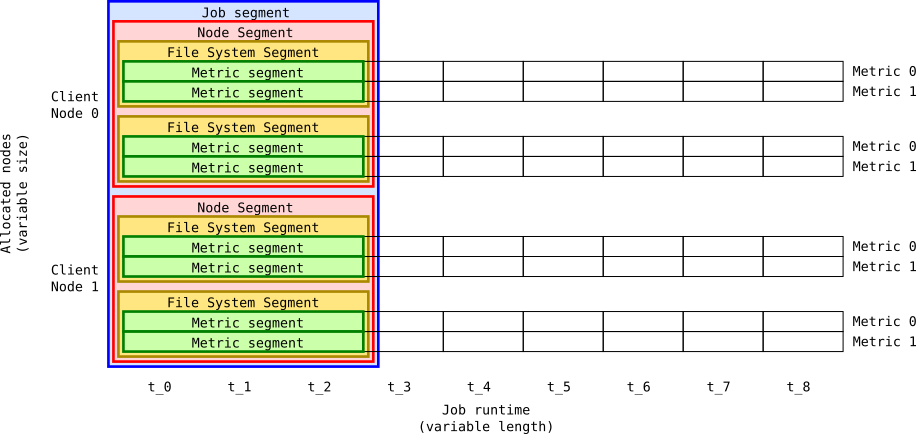
\includegraphics[width=0.9\textwidth]{assets/stats3.png}
 \caption{An example of 4-dimensional raw monitoring data (Node $\times$ File System $\times$ Metric $\times$ Time) and different levels of segmentation (colored boxes).}%
 \label{fig:generic_example}
\end{figure}

\paragraph{Segmentation.}
We split the time series of each I/O metric into equal-sized time intervals (segments) and computes a mean performance for each segment.
This stage preserves the performance units (e.g., Op/s, MiB/s) for each I/O metric.
The example in \Cref{fig:generic_example} creates segments out of three successive time points just for illustration purposes.
Depending on aggregation function, segments can be created of metrics (green boxes), of file systems (yellow boxes), of nodes (red boxes), or even over all dimensions (blue box).
The raw monitoring data is converted into a time series of ten minute segments, which we found is a good trade-off to sufficiently represent the temporal behavior of the application while it reduces the size of the time series.

\paragraph{Categorization.}
Next, to get rid of specific units of individual metrics, and to allow calculations between different I/O metrics, we introduced a categorization pre-processing step that takes into account the performance of the underlying HPC system and assigns a unitless ordered category to each metric segment.
For example, how could we compare the metric that reports 10k\,file opens with another metric that reports 100\,MB data was accessed?
We use three categories, which are the LowIO=0, HighIO=1 and CriticalIO=4 categories.
The category split points are based on the histogram of the indivudal metrics.
For any metrics, a segment with a value up to the 99\%-Quantile it is considered to be LowIO, larger than the 99.9\%-Quantile indicates CriticalIO, and between it is HighIO~(see \cite{iocats2020}).
This node-level data can then be used to compute job-statistics by aggregating across dimensions such as time, file systems, and nodes.


In summary, this data representation has the following key advantages for data analysis.
The ordered categories make the calculations between different metrics feasible, which is not possible with raw data.
Furthermore, the domains are equally scaled and compatible, because the values are between 0 and 4, and a value has a semantical meaning (low, high, or critical IO).
Besides, the resulting data representation is much smaller compared to the raw data.
This allows us to apply compute-intensive algorithms to large datasets.
Finally, as we are mostly interested in jobs with relevant IO, segments mapped to the LowIO category don't distract from significant parts of jobs.

In our previous work, we computed three high-level metrics per job that aid users to understand job profiles:

\begin{itemize}
	\item \textbf{Job-I/O-Balance:} indicates how I/O load is distributed between nodes.
	\item \textbf{Job-I/O-Utilization:} shows the average I/O load during I/O-phases.
	\item \textbf{Job-I/O-Problem-Time} is the fraction of job runtime that is I/O-intensive; it is approximated by the fractions of segments that are considered I/O intensive.
\end{itemize}

\begin{figure}[!bt]
	\centering
	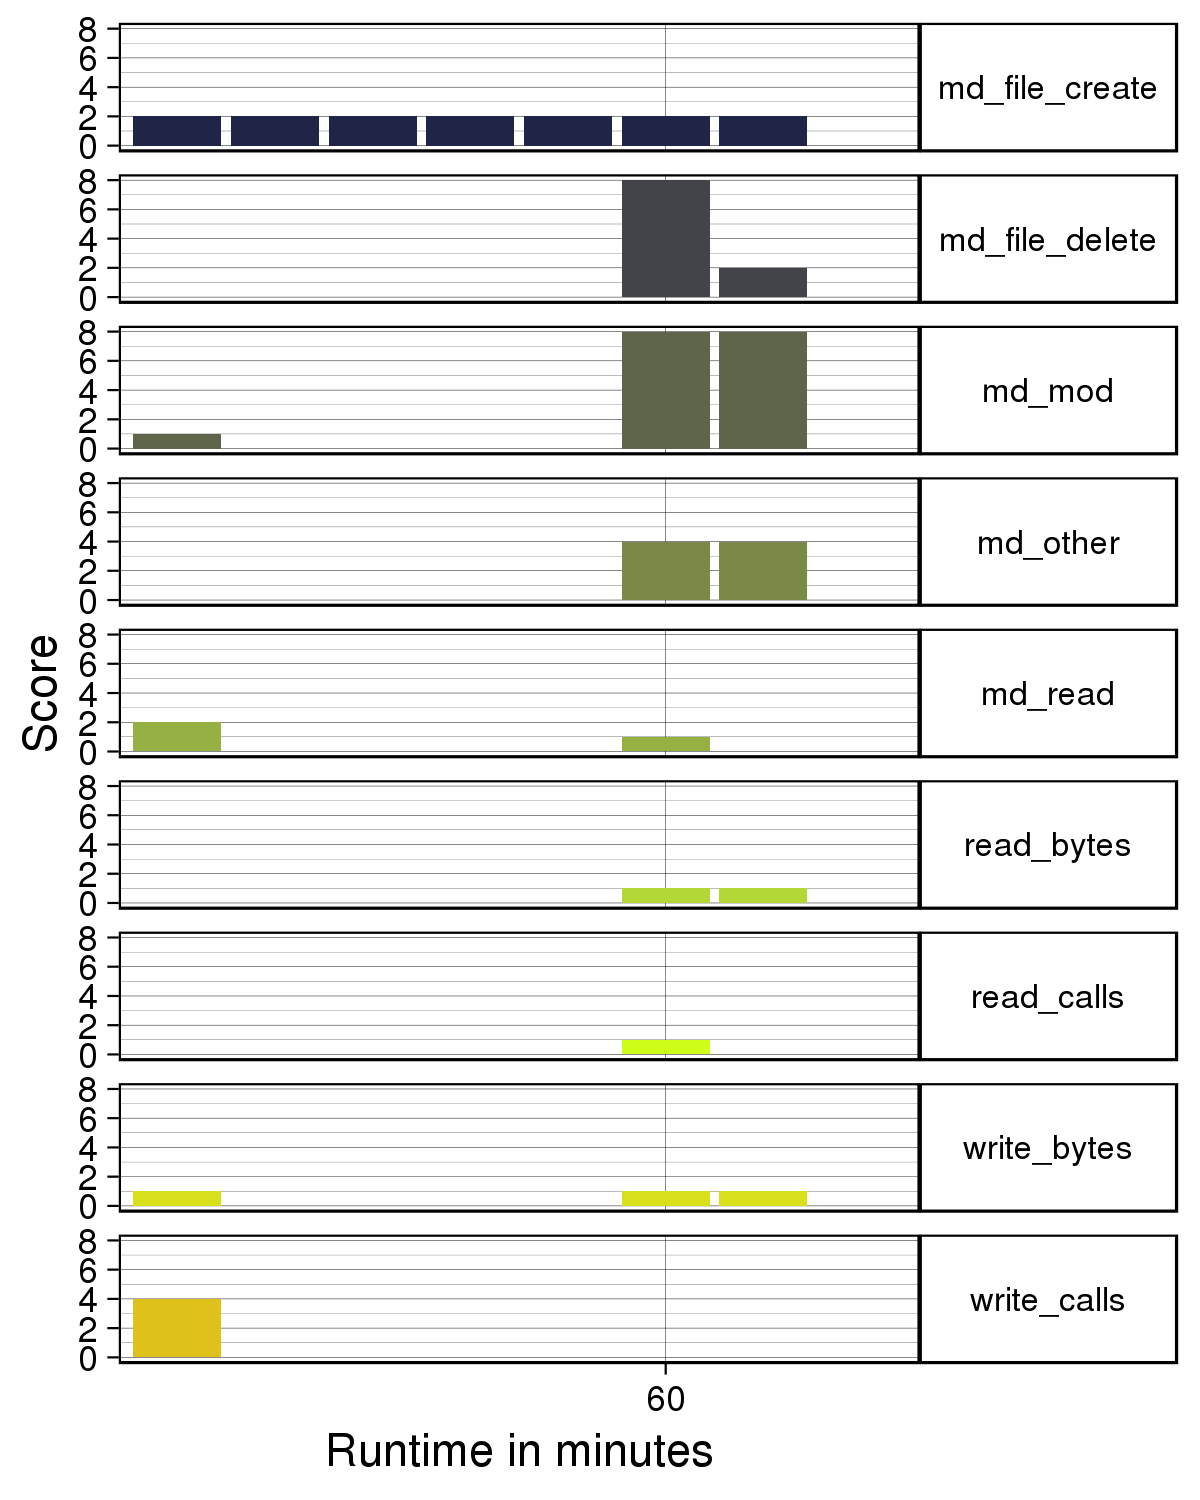
\includegraphics[width=2.75in]{image4.png}
	\caption{Example job-level metric.
Score is the sum of all node scores.}
	\label{fig:seg_example}
\end{figure}

In \Cref{fig:seg_example}, we can see the temporal behavior for this particular job when summing up the node-level metrics.
We call \textbf{an I/O phase a contiguous sequence of non-zero segments} (where the score of the segment is larger than zero).
For example, in the figure, we can see one phase for md\_file\_create, and two phases for md\_mod (one short and non-intrusive at the beginning, and one critical around 60 minutes).

When looking at categorization at the metric level, i.e., after reduction of the nodes and file system dimensions, we can observe that many jobs exhibit I/O phases.

\section{Similarity Between Jobs}%
\label{sec:job_similarity}

The raw monitoring data of a job in our environment at DKRZ, we obtain a time series of nine metrics per node, each metric sampled at five seconds intervals.
When comparing the time series of such metrics between two jobs, the key question is how do we define the similarity between multiple time series that may even be of different length.
ML techniques work well to deal with a fixed number of features, e.g., by creating a fixed-size profile for the jobs and applying dimension reduction techniques such as PCR, we could reduce the complexity and potentially obtain a similar representation for, e.g., two time series.

To understand which technique we should use, first, we need to discuss the perception of similarity of I/O patterns from the user perspective.
In \Cref{fig:typ_io:all}, we illustrate the time series of two metrics for three different jobs.
The figures show the typical behavior of parallel applications, computation is interrupted by regular I/O phases -- by phase, we mean a consecutive segment of time in which  certain behavior is exhibited, i.e., the statistics are similarly.

Actually, the shape of I/O phases depends on our definition of I/O phase.
By applying dimension reduction techniques, I/O phases from different dimensions can be joined together.
Although several aggregations are possible, in this work we focus on  I/O phases on metrics, i.e, we aggregate nodes and file system dimensions.
When investigating the distribution of I/O phases, we observe that jobs (longer than three segments) exhibit  several.

From the user support side, we might be interested in grouping similar suboptimal jobs and aim to provide one recipe to optimize all that exhibit such a behavior.
Similarly, we might be interested to optimize the pattern for a single I/O phase.
Optionally, we may be interested to ignore computation time and focus on I/O phases only.
Regardless of the segment of the time series we look at, we naively would consider an I/O pattern to be identical if the time series for all metrics of one job is identical to those of another job.
Unfortunately, the obtained measurements vary due to the nature of parallel applications and the environment of the data center they are executed:
In practice, different jobs show a different runtime, and even when re-running the same job, the obtained time series varies.

\begin{figure}
        \centering
         \begin{subfigure}[t]{\textwidth}
           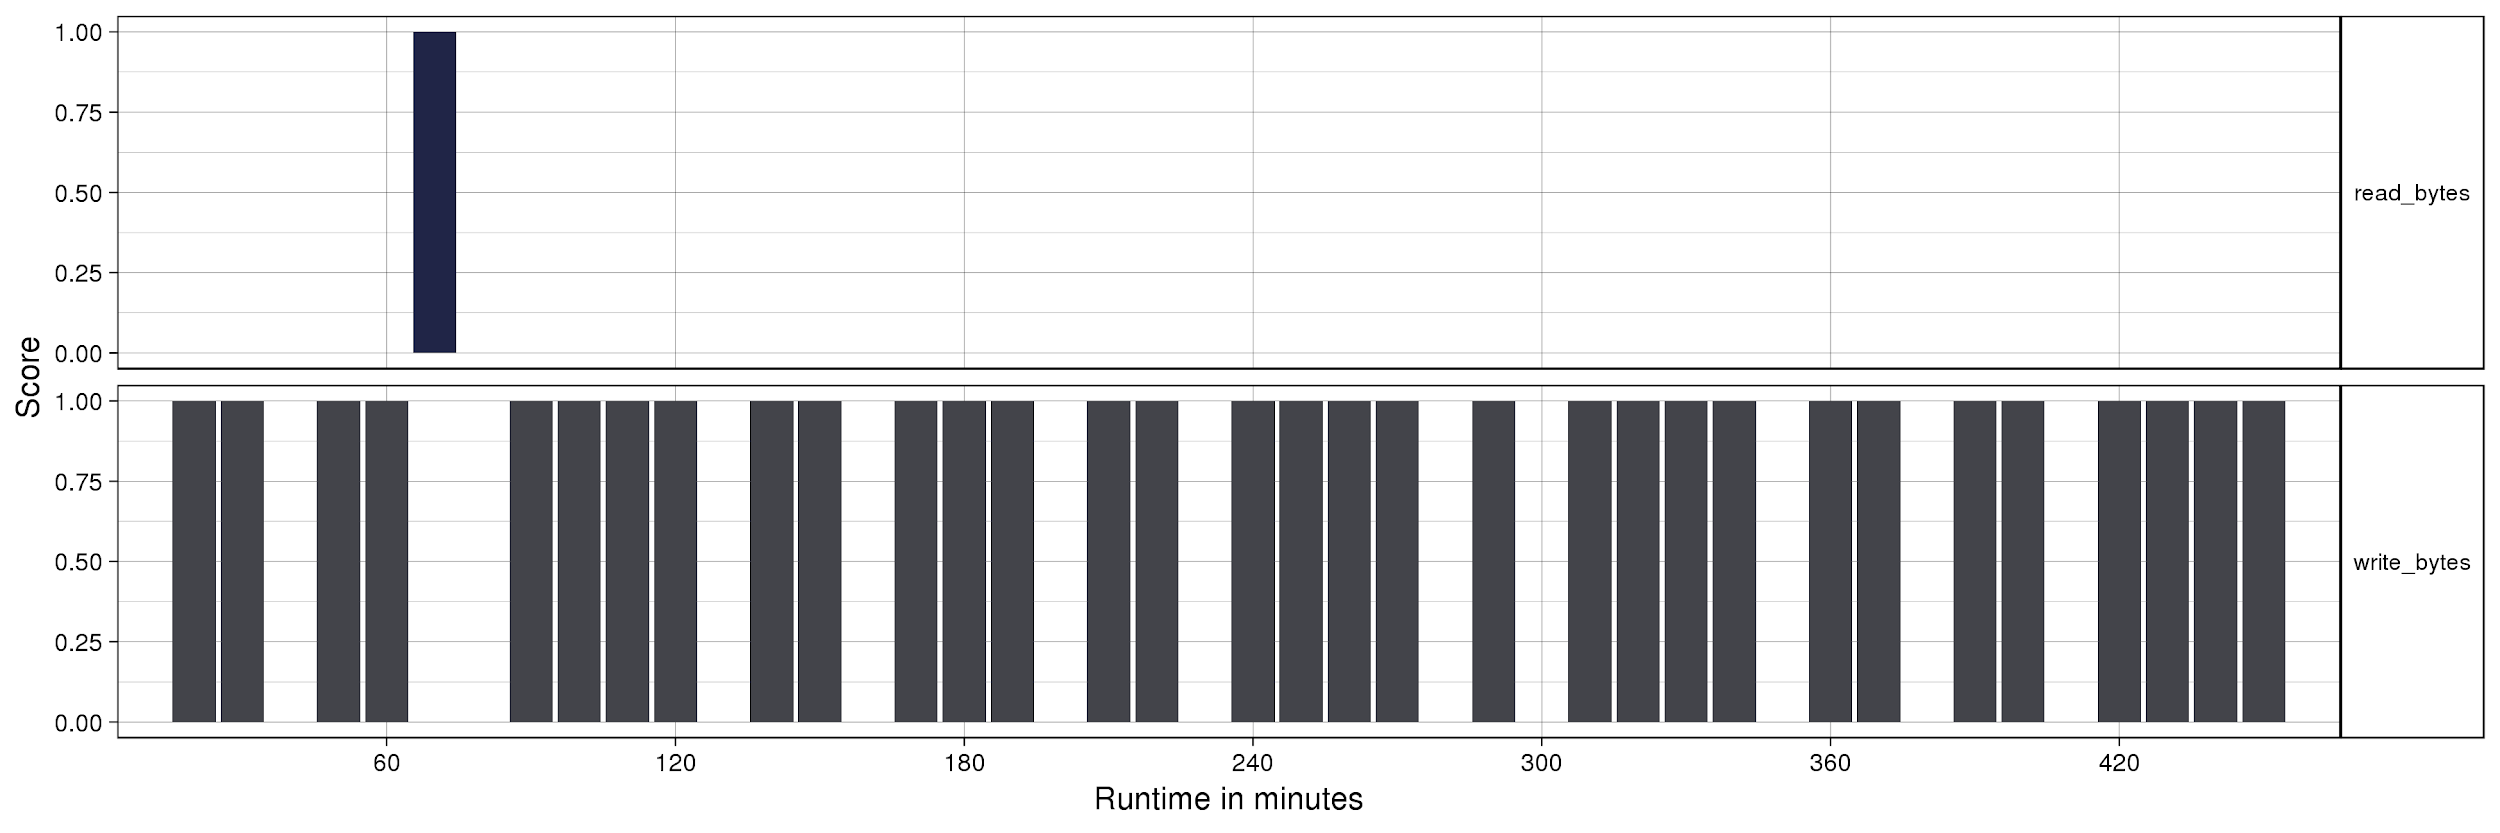
\includegraphics[width=\textwidth]{image27.png}
           \caption{Job A runs on 13 nodes}
           \label{fig:typ_io:1}
         \end{subfigure}

        \begin{subfigure}[t]{\textwidth}
           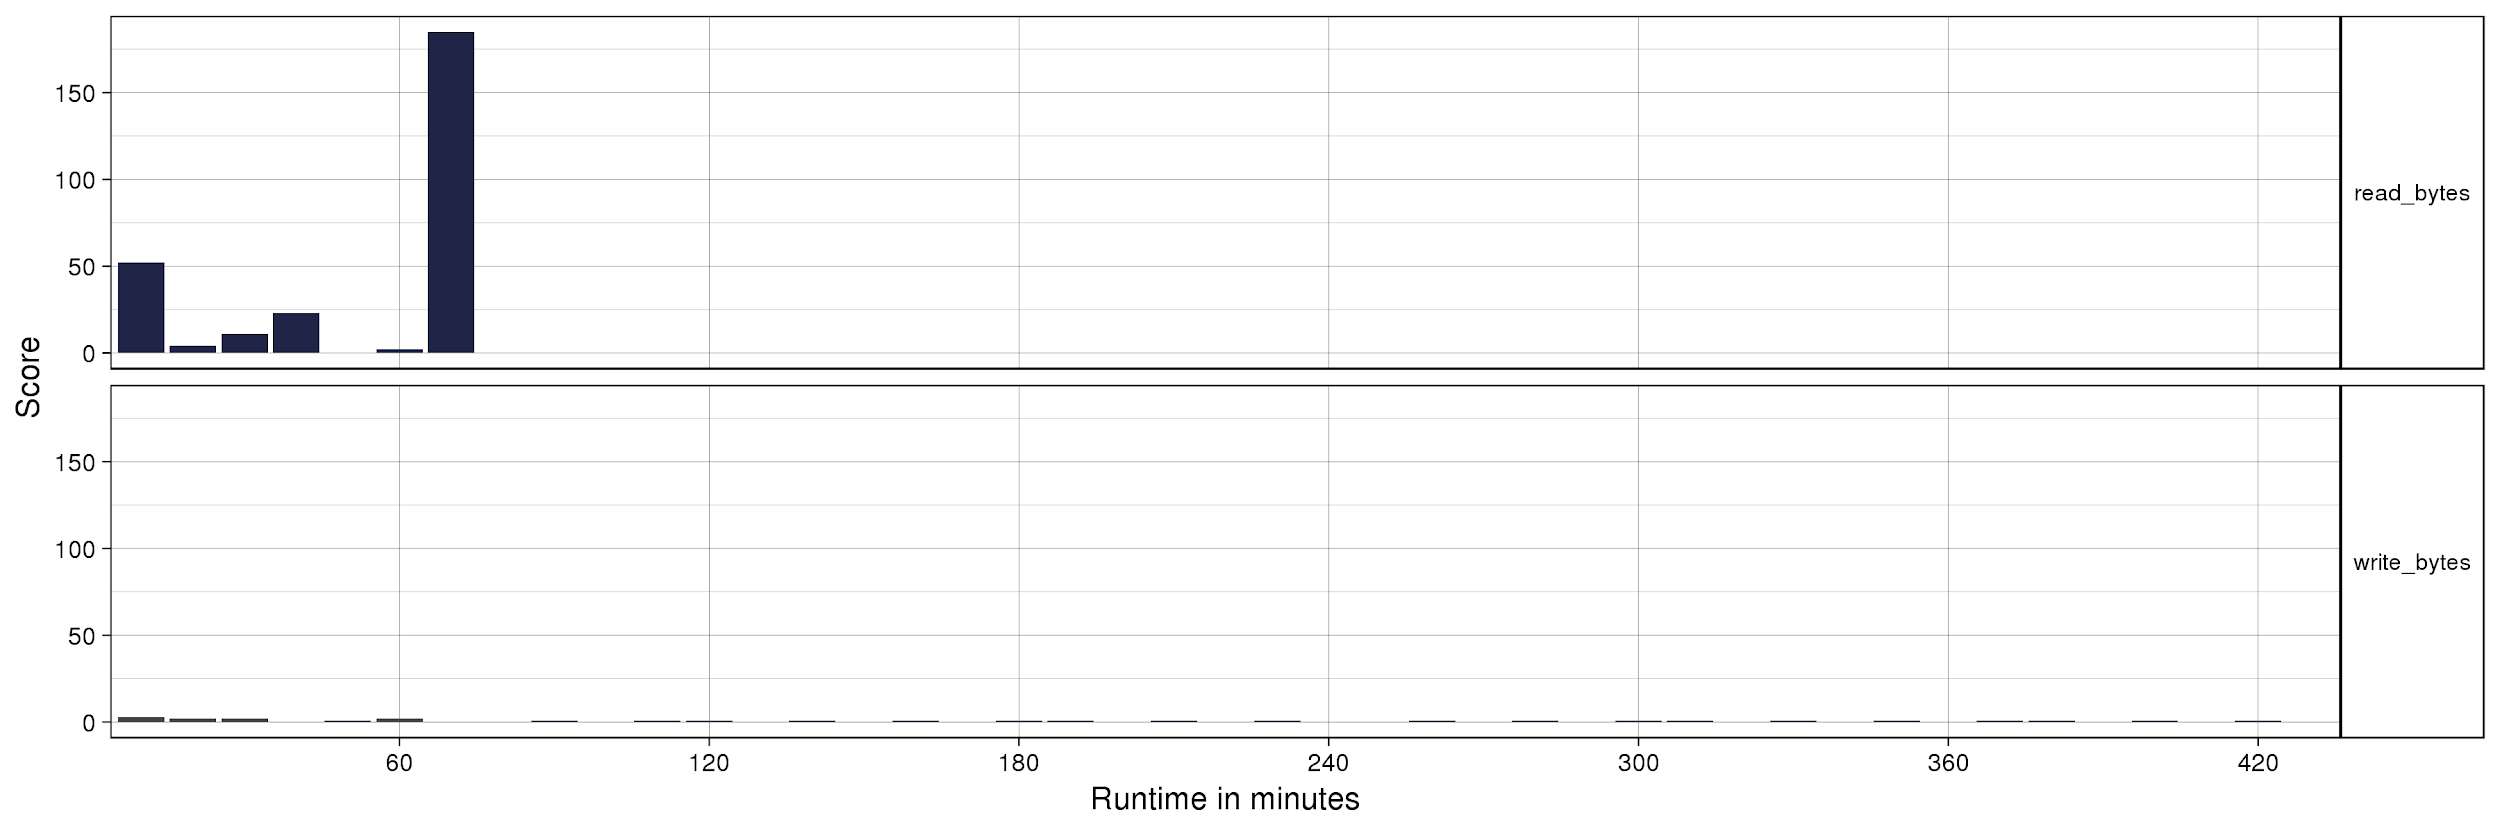
\includegraphics[width=\textwidth]{image28.png}
           \caption{Job B runs on 225 nodes}
           \label{fig:typ_io:2}
         \end{subfigure}

        \begin{subfigure}[t]{\textwidth}
          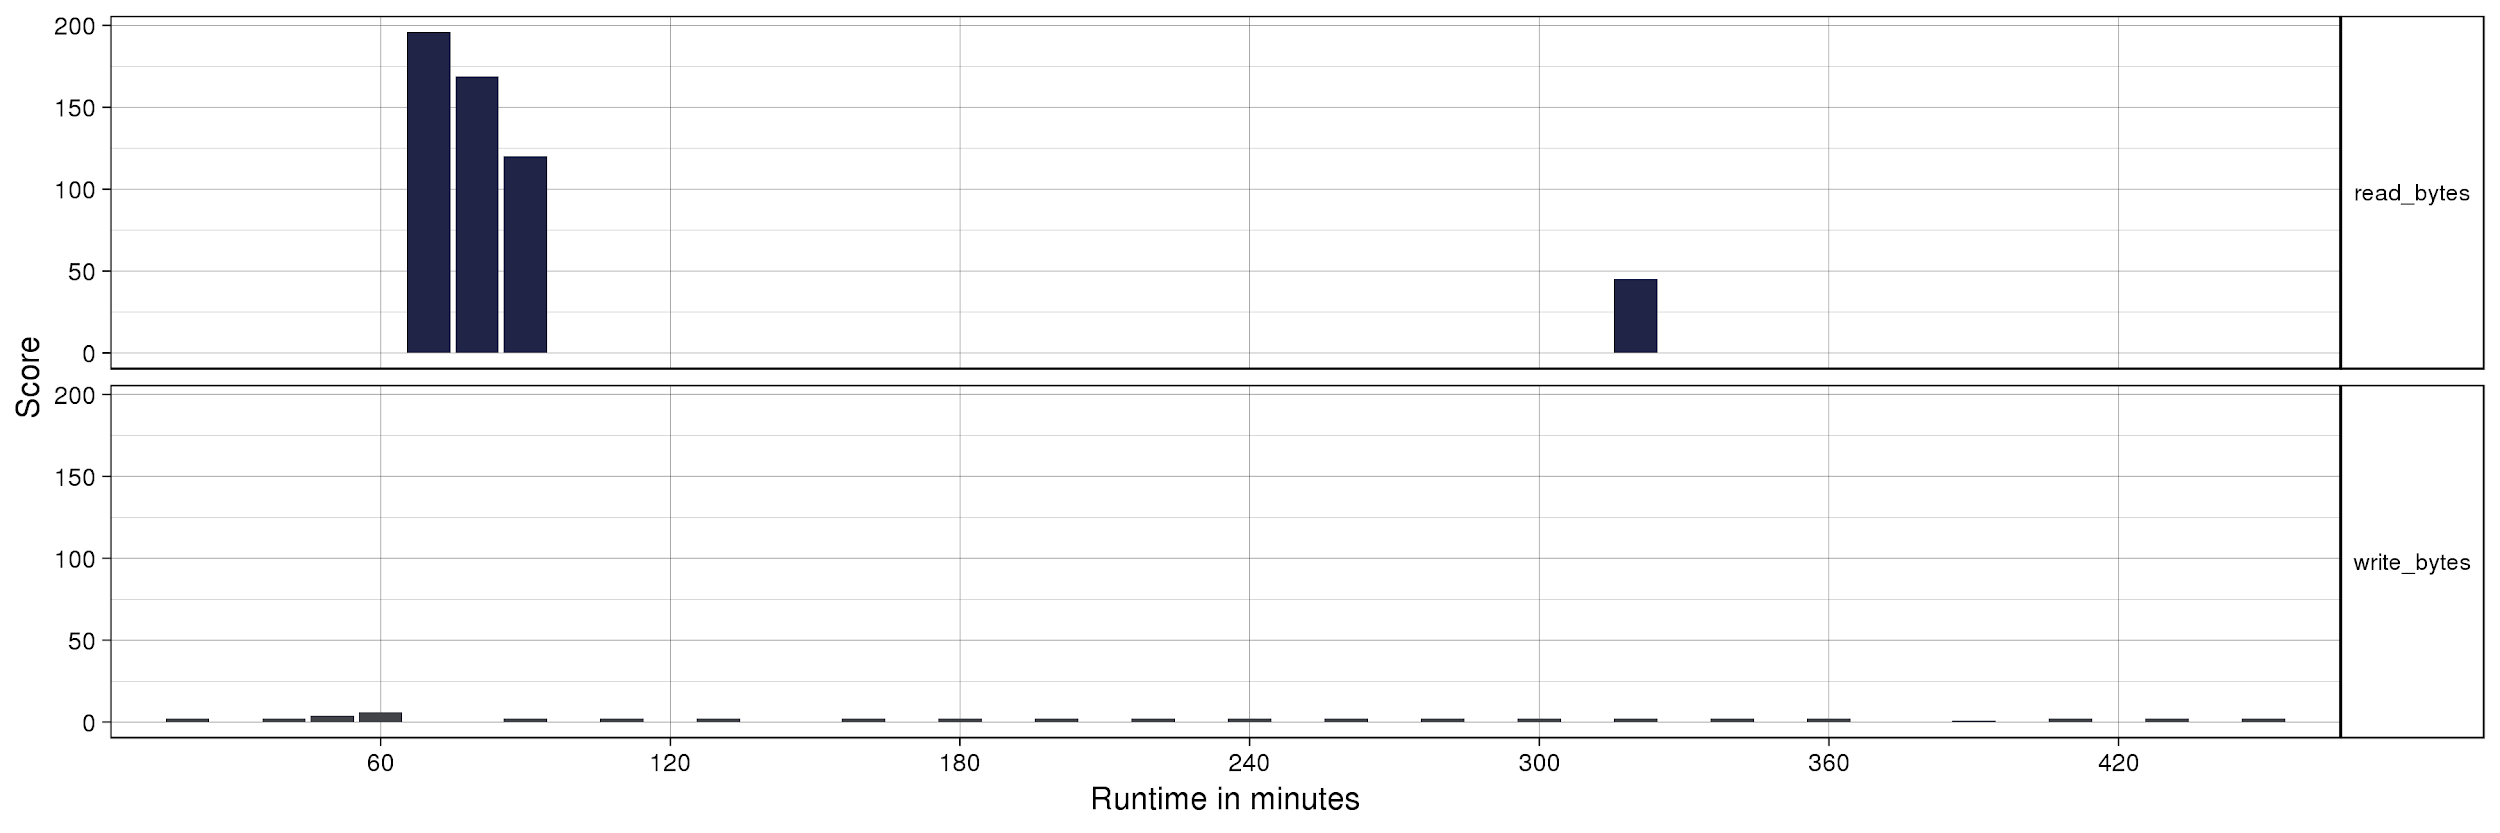
\includegraphics[width=\textwidth]{image25.png}
          \caption{Job C runs on 40 nodes}
          \label{fig:typ_io:3}
        \end{subfigure}
\caption{Monitoring data of three jobs.
Score is the sum of individual node scores.}
         \label{fig:typ_io:all}
\end{figure}

Typical sources of variability when observing performance metrics are: The concurrent usage of the shared storage, a shift between observed I/O phases due to network congestion or CPU throttling for power/heat reasons.
The same application using a different input configuration may need more compute time, resulting in longer phases between typical I/O patterns; moreover, it may change the I/O pattern.
A well-known pattern exhibited by a shorter running application may appear as well in a long-running application.
The similarity measure between two jobs should consider those sources of variability and allow us to provide a robust clustering of jobs depending on the user question.

There are different goals for the data analysis done by the user running the application or the support staff of the data center.
Whether the timeline is similar when executing an application with a different configuration and input dataset depends on the purpose of the analysis and task that follows the analysis.
For these reasons, we decided to explore a variety of alternative options for distance metrics and pre-processing and assess their suitability.


\section{Related Work}%
\label{sec:rel_work}
There are many tracing and profiling tools that are able to record I/O information~\cite{TFAPIKBBCF19}; we will discuss a selection of them in more detail in the following.
Most of them focus on individual jobs, and only a few of them apply machine learning for data analysis, in particular across jobs.
As the purpose of applications is computation and, thus, I/O is just a byproduct, applications often spend less than 10\% time with I/O.
The issue of performance profiles is that they remove the temporal dimension and make it difficult to identify relevant I/O phases.
The Ellexus tools\footnote{\url{https://www.ellexus.com/products/}} include Breeze, a user-friendly offline I/O profiling software, an automatic I/O report generator Healthcheck, and command line tool Mistral which purpose is to report on and resolve I/O performance issues when running complex Linux applications on high performance compute clusters.
Mistral is a small program that allows you to monitor application I/O patterns in real time, and log undesirable behaviour using rules defined in a configuration file called a contract.

Darshan~\cite{carns2011understanding-toc,hpcdarshan} is an open source I/O characterization tool for post-mortem analysis of HPC applications' I/O behavior.
Its primary objective is to capture concise but useful information with minimal overhead.
Darshan accomplishes this by eschewing end-to-end tracing in favor of compact statistics such as elapsed time, access sizes, access patterns, and file names for each file opened by an application.
These statistics are captured in a bounded amount of memory per process as the application executes.
When the application shuts down, this data is reduced, compressed, and stored in a unified log file.
Utilities included with Darshan can then be used to analyze, visualize, and summarize the Darshan log information.
Because of Darshan's low overhead, it is suitable for system-wide deployment on large-scale systems.
In this deployment model, Darshan can be used not just to investigate the I/O behavior of individual applications but also to capture a broad view of system workloads for use by facility operators and I/O researchers.


There are approaches that monitor record storage behavior and aim to identify inefficient applications in a cluster.
TOKIO~\cite{lockwood2018tokio} integrates logs from various sources to allow an analysis of data.
It allows finding certain inefficient access patterns in the data.

The LASSi tool~\cite{DBLP:journals/corr/abs-1906-03884} was developed for detecting, the so called, victim and aggressor applications.
An aggressor can steal I/O resources from the victim and negatively affect its runtime.
To identify such applications, LASSi calculates metrics from Lustre job-stats and information from the job scheduler.
One metric category shows file system load and another category describes applications I/O behavior.
The correlation of these metrics can help to identify applications that cause the file system to slow down.
In the LASSi workflow this is a manual step, where a support team is involved in the identification of applications during file system slow down.
Manual steps are disadvantageous when processing large amounts of data and must be avoided in unsupervised I/O behavior identification.
LASSi's indicates that the main target group are system maintainers.
Understanding LASSi reports may be challenging for ordinary HPC users, who do not have knowledge about the underlying storage system.


In~\cite{TUISVPKB19}, the authors utilized probes to detect file system slow-down.
A probing tool measures file system response times by periodically sending metadata and read/write requests.
An increase of response times correlates to the overloading of the file system.
This approach allows the calculation of a slow-down factor identification of the slow-down time period.
This approach is able to detect a file system slow-down, but cannot detect the jobs that cause the slow-down.

The Nextgenio monitoring system~\cite{nextgenio2016}, has four main collectors.
The first two, the PBS and ALPS tools, collect job scheduling information.
The proprietary Cray I/O monitoring tool exploits Lustre I/O counters to capture file system usage on OSTs of all OSSs and allocated compute nodes.
The MAP component provides information about CPU, memory and network usage.
Then all the collected data is clustered for the analysis of system usage and performance evaluation.
In contrast to existing approaches, our approach focuses on the analysis of job data and investigates clustering strategy to group similar jobs.


HiperJOBVIZ~\cite{hiperjobviz2019} is a visual analytic tool for visualizing the resource allocations of data centers for jobs, users, and usage statistics.
It provides an overview of the current resource usage and a detailed view of the resource usage via multi-dimensional representation of health metrics.
TimeRadar\footnote{\url{https://idatavisualizationlab.github.io/HPCC/TimeRadar}} is a part of the tool, which summaries the resource usage via radar charts, creating a kind of comprehensible profile for different user groups.

Trace analysis tools such as Vampir~\cite{nagel1996vampir} offer clustering strategies to analyze the per-process time series of a single job, in particular to group similar time series and allow users to focus on the exceptional cases that may lead to slowdown of the parallel application.
In \cite{weber2016structural}, a strategy is developed for determining such a clustering based on execution structure; the paper gives a good introduction for the comparison of two traces as well.

In contrast to existing strategies, we compare a large number of jobs with individual properties.

\section{Methodology}%
\label{sec:methodology}

The goal of this article is to research the impact of clustering strategies on many jobs from the perspective of a user and data center.
Generally, machine learning algorithms expect a fixed number of features, therefore, the time series of statistics that is retrieved on the node-level needs to be pre-processed.
The application of a “specific algorithm” can be understood as a number of successive processing steps on data.
Roughly speaking, there are three basic steps: data pre-processing (including coding), similarity computation, and clustering.
We call one algorithm representing such a combination a \textit{clustering stack}.
The pre-processing converts the dynamic-sized monitoring data which depends on the number of captured metrics, allocated nodes, and application runtime into a suitable representation for the clustering algorithm.
Then the clustering is applied using a specific similarity function.
Finally, the quality of the clustering result is assessed, i.e., how suitable is this strategy for our I/O statistics and use cases?

\subsection{Overview}

In the following, we have dedicated a section to each step in the analysis.
We are listing and briefly discussing potential alternatives.
The list of alternatives does not intend to be complete but shows a variety of options.

\subsubsection{Data pre-processing}
The 4-dimensional data from our monitoring system is too fine-grained for mass analysis,
to be able to analyze millions of jobs, we must apply some data reduction technique.
The result of the data-preprocessing is a coding of the initial time series data into one or multiple vectors.

We first convert the time series into segments of ten minutes which we found previously is a good trade-off to represent the temporal behavior of the application while it reduces the size of the time series.
Hence, for a job and for each of our nine client-side recorded metrics, we obtain a coarse-grained time series.
To simplify the interpretation of results and the choice distance metrics, it is beneficial to have the same unit for all features which is why we use our category classification which creates a unitless order.
For example, when reduced by node, file system, and across metrics, a point may represent the mean value across all time series for the job for the ten minutes interval.

On the high-level, the following strategies for data reduction could be considered:
\begin{itemize}
	\item \textbf{Job profiles} compute a fixed set of statistics across the whole job regardless of dynamic factors such as runtime or nodes by applying reduction operations such as the arithmetic mean.
		A drawback of this simplification is that any temporal pattern is lost.
	\item \textbf{Segment statistics} compute for each segment a fixed statistics, such as the mean value across all nodes.
		This basically preserves the time series and depends on the job-length.
	\item \textbf{Phase statistics} computes high-level statistics by analyzing the temporal behavior of I/O phases further, e.g., compute the average length of IO segments with CriticalIO.
		This approach is independent of the job length but requires identifying phases and determining meaningful job metrics.
\end{itemize}

We decided to distinguish the different dimensions of a job (Node, File System, Metric, and Time) defining how the aggregation is performed.
Not reducing data in the dimension would mean that the result would depend on, e.g., the number of nodes of a job, which makes the comparison of two jobs difficult.
For one dimension, you could compute various statistics; we decided to use mean or sum.
Any data reduction is performed in this order across the dimensions: first File System, Node, and last by Metric.
Thus, a time series of encoded segments remain.
The time series of segments can be reduced differently in each dimension; alternatives that we apply in this paper are listed in \Cref{tab:reduction_techniques}.
By reducing along all dimension, you obtain basically a job profile (as discussed above).

\begin{table}
	\centering
	\begin{tabularx}{\textwidth}{llX}
		Dimension       & Operation                                    &  Description                                   \\
		\midrule
		Node            & Reduce by mean()                             &  Aggregate all nodes by mean() function        \\
		                & Reduce by sum()                              &  Aggregate all nodes by sum() function         \\
		File System     & Reduce by mean()                             &  Aggregate all file systems by mean() function \\
		                &
		Reduce by sum() & Aggregate all file systems by sum() function \\
		Metric          & Reduce by sum()                              &  Aggregate all nine metrics by sum()           \\
		Time            &                                              &  Convert segments to coding formats            \\
		All             & Reduce by mean()                             &  Reduces time series to a fixed set of values  \\
	\end{tabularx}
	\caption{Dimension reduction strategies for the original 4D-data.}
	\label{tab:reduction_techniques}
\end{table}

\subsubsection{Coding}


Segmented data contains a numeric floating-point value for each data, which can be too much information for the analysis.
Therefore, we introduce two condensed data representations called binary and hexadecimal coding.
Additionally, we introduce two operations on the coding:
the first extracts I/O phases -- a phase is a consecutive non-zero series of segments;
the second merges all consecutive zero segments into one segment, i.e., removes compute phases in the statistics.
The operations are summarized in \Cref{tab:coding_ops} and described in the following.

\begin{table}[t]
 \centering
 \begin{tabularx}{\textwidth}{lX}
	 Operation &  Description \\
	 \midrule
	 Binarization & Segments are mapped to 9-bit numbers (v), where each position (i) represents a metric.
The bits are set by the following function:

	 \vbox{
		\begin{equation}
			v_i =
			\begin{cases}
				\text{false if segment}_i = 0\\\text{true otherwise.}
			\end{cases}, i \in [\text{enumerated metrics}]
		\end{equation}
	 } \\[-1em]
	 Hex-Quantization & Quantize segments to NonIO + 16 I/O levels.\\
	 Zeros-Aggregation & Merge all consecutive zero segments.\\
	 Phase-Extraction &  Extract continuous sequences of non-zero segments.
\par - Split time series at zero segments in sub time series (I/O phases) and remove zero segments.
\par - Preserve order of I/O phases.\\
 \end{tabularx}
 \caption{Coding operations.}
 \label{tab:coding_ops}
\end{table}

\paragraph{Binary coding}
Binary coding represents monitoring data as a sequence of numbers, where each number represents the overall file system usage.
The number is computed based on the nine metrics found in the segment, e.g., if a phase is read-intense and write-intense, it is encoded as one type of behavior.
In this approach, each conceivable combination of activities has a unique number.

The approach maps the three categories to the following two states: The LowIO category is mapped to the non-active (0) state, and HighIO and CriticalIO categories are mapped to the active (1) state.
On one side, by doing this, we lose information about performance intensity, but on other side, this simplification allows a more comprehensible comparison of job activities.

In our implementation, we use a 9-bit number to represent each segment, where each bit represents a metric.
The bit is 1 if the corresponding metric is active, and 0 if not.
Translated to the decimal representation, metric segments can be coded as 1, 2, 4, 8, 16, and so on.
Using this kind of coding we can compute a number for each segment, that describes unambiguously the file system usage, e.g., a situation where intensive usage of md\_read (Code=16) and read\_bytes (Code=32) occur at the same time and no other significant loads are registered is coded by the value 48.
Coding is reversible, e.g., when having value 48, the computation of active metrics is straightforward.

%\begin{table}[H]
%       \centering
%\begin{tabular}{p{0.8in}p{0.8in}}
%\hline
%%row no:1
%\multicolumn{1}{p{0.8in}}{\cellcolor[HTML]{C9DAF8} \tabto{0.25in}  \tabto{0.39in} \tab Metric} &
%\multicolumn{1}{p{0.8in}}{\cellcolor[HTML]{C9DAF8} \tabto{0.25in}  \tabto{0.39in} \tab Code} \\
%\hhline{--}
%%row no:2
%\multicolumn{1}{p{0.8in}}{md\_file\_create} &
%\multicolumn{1}{p{0.8in}}{ \tabto{0.25in}  \tabto{0.39in} \tab 1} \\
%\hhline{~~}
%%row no:3
%\multicolumn{1}{p{0.8in}}{md\_file\_delete} &
%\multicolumn{1}{p{0.8in}}{ \tabto{0.25in}  \tabto{0.39in} \tab 2} \\
%\hhline{~~}
%%row no:4
%\multicolumn{1}{p{0.8in}}{md\_mod} &
%\multicolumn{1}{p{0.8in}}{ \tabto{0.25in}  \tabto{0.39in} \tab 4} \\
%\hhline{~~}
%%row no:5
%\multicolumn{1}{p{0.8in}}{md\_other} &
%\multicolumn{1}{p{0.8in}}{ \tabto{0.25in}  \tabto{0.39in} \tab 8} \\
%\hhline{~~}
%%row no:6
%\multicolumn{1}{p{0.8in}}{md\_read} &
%\multicolumn{1}{p{0.8in}}{ \tabto{0.25in}  \tabto{0.39in} \tab 16} \\
%\hhline{~~}
%%row no:7
%\multicolumn{1}{p{0.8in}}{read\_bytes} &
%\multicolumn{1}{p{0.8in}}{ \tabto{0.25in}  \tabto{0.39in} \tab 32} \\
%\hhline{~~}
%%row no:8
%\multicolumn{1}{p{0.8in}}{read\_calls} &
%\multicolumn{1}{p{0.8in}}{ \tabto{0.25in}  \tabto{0.39in} \tab 64} \\
%\hhline{~~}
%%row no:9%\multicolumn{1}{p{0.8in}}{write\_bytes} &%\multicolumn{1}{p{0.8in}}{ \tabto{0.25in}  \tabto{0.39in} \tab 128} \\
%\hhline{~~}
%%row no:10
%\multicolumn{1}{p{0.8in}}{write\_calls} &
%\multicolumn{1}{p{0.8in}}{ \tabto{0.25in}  \tabto{0.39in} \tab 256} \\
%\hhline{~~}
%\end{tabular}
% \end{table}

To reduce the 4-dimensional data, we reduce that structure to two dimensions (segments metrics) by aggregating other dimensions by applying sum() function on score values.
In the resulting table we leave zero scores, and change scores larger than zero to one.
After coding each segment, the jobs can be represented as a sequence of numbers, e.g.,

\begin{lstlisting}[caption={Binary coding of a 15 segments long job.}]
[1:5:0:0:0:0:0:0:96:96:96:96:96:96:96]
\end{lstlisting}

The monitoring dataset doesn't provide information about what happens during the zero segments.
It can be anything, like a job is waiting for resources, or computing something.
It can also be that the job script cannot start immediately or run on a slow network.
To catch such jobs, we aggregate multiple consecutive zero segments into one zero segment, thus the coding of the previous job would replace all 0:...:0 sequences just with one 0.

\begin{lstlisting}[caption={Binary coding of a 15 segments long job with zero aggregation applied.}]
[1:5:0:96:96:96:96:96:96:96]
\end{lstlisting}

Note, that the actual job length is kept for analysis purpose, thus, only the length of the encoded sequence changes.

\paragraph*{Hexadecimal coding}

This coding preserves monitoring data for each metric and each segment.
As the name suggests, the value of a segment is converted into a hexadecimal number to allow creation of a string representing the I/O behavior.
The numbers are obtained in two steps.
Firstly, the dimension reduction aggregates the file system and the node dimensions and computes a mean value for each metric and segment, which lies in the interval [0,4].
%Secondly, the mean values are quantized into NonIO + 16 I/O levels -- 0 (NonI0) represents the interval [0,0.25), 1 = [0.25,0.625), 2 = [0.625,0.825) $ \ldots $, e = [XX, XX), f = [3.875,4].
Secondly, the mean values are quantized into one NonIO level and 16 I/O levels (\Cref{tab:quant_intervals}).
The example below shows hexadecimal coding for a job containing 6 segments.

\begin{table}
\begin{tabular}{lll}
Level & Interval      & Interval Size \\ 
\midrule
0     & [0,0.125)     & 0.125         \\ 
1     & [0.125,0.375) & 0.25          \\ 
2     & [0.375,0.625) & 0.25          \\ 
3     & [0.625,0.875) & 0.25          \\ 
4     & [0.875,1.125) & 0.25          \\ 
5     & [1.125,1.375) & 0.25          \\ 
6     & [1.375,1.625) & 0.25          \\ 
7     & [1.625,1.875) & 0.25          \\ 
8     & [1.875,2.125) & 0.25          \\ 
9     & [2.125,2.375) & 0.25          \\ 
10    & [2.375,2.625) & 0.25          \\ 
11    & [2.625,2.875) & 0.25          \\ 
12    & [2.875,3.125) & 0.25          \\ 
13    & [3.125,3.375) & 0.25          \\ 
14    & [3.375,3.625) & 0.25          \\ 
15    & [3.625,3.875) & 0.25          \\ 
16    & [3.875,4]     & 0.125         \\ 
\end{tabular}
\caption{Non-uniform quantization intervals}
\label{tab:quant_intervals}
\end{table}


\begin{lstlisting}[caption={Hexadecimal coding of a six segments long job.}]
'md_file_create' : [0:0:2:2:2:9]
'md_file_delete' : [0:0:0:0:0:0]
'md_mod'         : [0:0:0:0:0:0]
'md_other'       : [0:0:0:0:0:0]
'md_read'        : [0:0:0:9:3:0]
'read_bytes'     : [5:0:0:0:0:0]
'read_calls'     : [0:0:0:0:0:0]
'write_bytes'    : [0:0:0:0:f:f]
'write_calls'    : [0:0:0:0:0:0]
\end{lstlisting}

\subsubsection{Similarity Metrics}
Determining the resemblance between two jobs is the main task of this work.
Clustering algorithms need a distance metrics to allow organizing them together.
There are various variants, a selection is listed in \Cref{tab:sim_funcs}.
The Eucledian distance for two vectors can naturally only be applied to vectors of the same length.
The Levenshtein distance is the number of modifications (inserts, deletes, changes) of individual characters that need to be made to transform one string to another.
It can also by applied on other data types such as vector and time series.

The Normalized-Difference and Relative-Change distances work with single values, and can not be applied directly on time series.
To make them work with time series we use the following approach.
Firstly, we introduce in \Cref{tab:matching_strategies} two additional operations that transform time series to the same length.
The first operation, Trimming, can remove segments at the beginning, or/and at the end of the longer job.
The second operation, Zeros-Insertions, can insert zero-segmens at the beginning, between, or/and at the end of I/O phases of both jobs.
Both operations create equal sized time series with the highest possible similarity.
Finally, we use a Normalized-Difference-based or Relative-Change-based similarity functions to compute similarity between segments, and obtain the overall similarity by computing the mean.

\begin{table}
  \centering
  \begin{tabularx}{\textwidth}{lllX}
    Distance              & Formula                                       & Domain                  & Description                                                                                    \\
    \midrule
    Euclidean             & $d_{\text{e}} =\sqrt{(\sum_i^n (a_i - b_i))}$ & $a, b \in \mathbb{R}^n$ & The Euclidean distance between two vectors.                                                    \\
    Levenshtein           & $d_{\text{lev}} = \text{lev}(a, b)$           & $a, b \in$ Time Series  & Number of operation (inserts, deletes, and changes) requires to convert one coding in another. \\
    Normalized-Difference & $d_{\text{nd}} = \frac{|a - b|}{16}$          & $0 \le a, b \le 16$     & A change from level 2 to level 6 on a 16 level system would be (6 - 2) / 16 = 0.25.            \\
    Relative-Change       & $d_{\text{rc}} = \frac{\min(a,b)}{\max(a,b)}$ & $a, b \in \mathbb{R}^+$ & A change from level 2 to level 6 system would be 2/6 = 0.66.                                   \\
  \end{tabularx}
  \caption{Selection of distance metrics that can be used to compute similarities.}
  \label{tab:sim_funcs}
\end{table}

\begin{table}
  \centering
    \begin{tabularx}{\textwidth}{lX}
      Operation       & Description                                                                                  \\
      \midrule
      Trimming        & Remove segments at the beginning or/and at the end of the longest time series. \\
      Zeros-Insertion & Insert zero-segments at the beginning, between I/O phases, or/and at the end of time series. \\
    \end{tabularx}
    \caption{Potential length adjustment strategies create time series with the same length.}
  \label{tab:matching_strategies}
\end{table}

\subsubsection{Clustering}
In the last step, similar jobs need to be grouped in clusters.
A subset of potential strategies is listed in \Cref{tab:clustering_algorithms}.
Often, the k-means algorithm is applied which utilizes a random strategy to initialize clusters.
However, as it requires us to define a fixed number of clusters, it is problematic as the number of actual clusters are unknown.
The large class of density clustering algorithms such as DBSCAN groups objects that are "close" together into one class; a user defines the maximum distance of objects that belong to the same class by setting an $\epsilon$ which represents the similarity value.
Agglomerative strategies group similar elements together to form a hierarchy of some sort, e.g., a tree.
Unfortunately, their complexity is quadratic at least.
To handle millions of jobs, an algorithm must be performant.

We developed two strategies that address the performance issue and the other limitations, the Clustering-Tree algorithm and the SimplifiedDensity algorithm.
These algorithms are able to handle the large number of jobs but aim to preserve the core ideas of k-means/density algorithms.
They are described in the following:

\begin{table}
  \centering
  \begin{tabularx}{\textwidth}{lX}
    Algorithm & Description \\
    \midrule
    k-means & Runs a random initialization, then refines the clusters until the clusters don't change further.\\
    Density clustering &  Group nearby elements recursively together as long as they are ($\epsilon$) close together.\\
    Agglomerative &  Hierarchically cluster data into groups of elements that belong closer together.\\
    \textbf{Clustering-Tree} &  Create a hierarchical clustering for subset of data to train a decision tree, then apply the decision tree on the full dataset.\\
    \textbf{Simplified-Density} &  Combines ideas from k-means with density clustering.
The simplified clustering algorithms add a job to a cluster if similarity to the cluster centroid is equal or larger than the user defined similarity (SIM) value.\\
  \end{tabularx}
  \caption{Selection of clustering algorithms}
  \label{tab:clustering_algorithms}
\end{table}
\paragraph{Clustering-Tree algorithm}
This algorithm involves three steps:

\begin{enumerate}
 \item Agglomerative clustering of a small dataset, enumerate similar leaf-level clusters.
 \item Training of a decision tree model on the small dataset, i.e., the tree should decide in which cluster a job is stored.
 \item Clustering of the large data set using the decision tree.
\end{enumerate}

Since the number of clusters on leaf-level depends on their similarity, this strategy should determine a number of suitable clusters that mimics the job distribution in the training set.

\paragraph{Simplified-Density algorithm}

The algorithm forms clusters around centroids.
These are job codings that form clusters by attracting similar jobs.
All jobs in a cluster fulfill only one condition, the similarity (SIM) to the centroid has to be bigger than the user defined minimum, in that sense it shares some similarity to DBSCAN.
It is approximative as the order of jobs matters for the creation of the clusters.

The algorithm can be summarized as follows:
\begin{enumerate}
 \item Pick one arbitrary job from the dataset, which will serve as a cluster centroid, and compute similarity to all other jobs.
 \item Create a cluster of jobs that have a minimum similarity and remove them from the dataset.
 \item Repeat step 1 and 2 until no jobs are left in the dataset.
\end{enumerate}

This approach allows a performant implementation, but they also allow a job to be in one cluster, even if a centroid of another cluster is much closer, as long as the condition is true.
Hence, the result depends on the processing order of the jobs, though it is deterministic.


\subsubsection{Clustering Stacks}
There are various combinations of the different strategies possible.
For simplicity, we refer to one clustering stack just as algorithm.
During our research, we explored various combinations out of the possible combinations, but we found that these do not perform well and are not interesting to discuss.
The operation stack which we describe in this article is visualized in \Cref{fig:clustering_stacks}.
In brief, the algorithms can be characterized like in \Cref{tab:alg_character}.

\begin{figure}[ht]
  \centering
  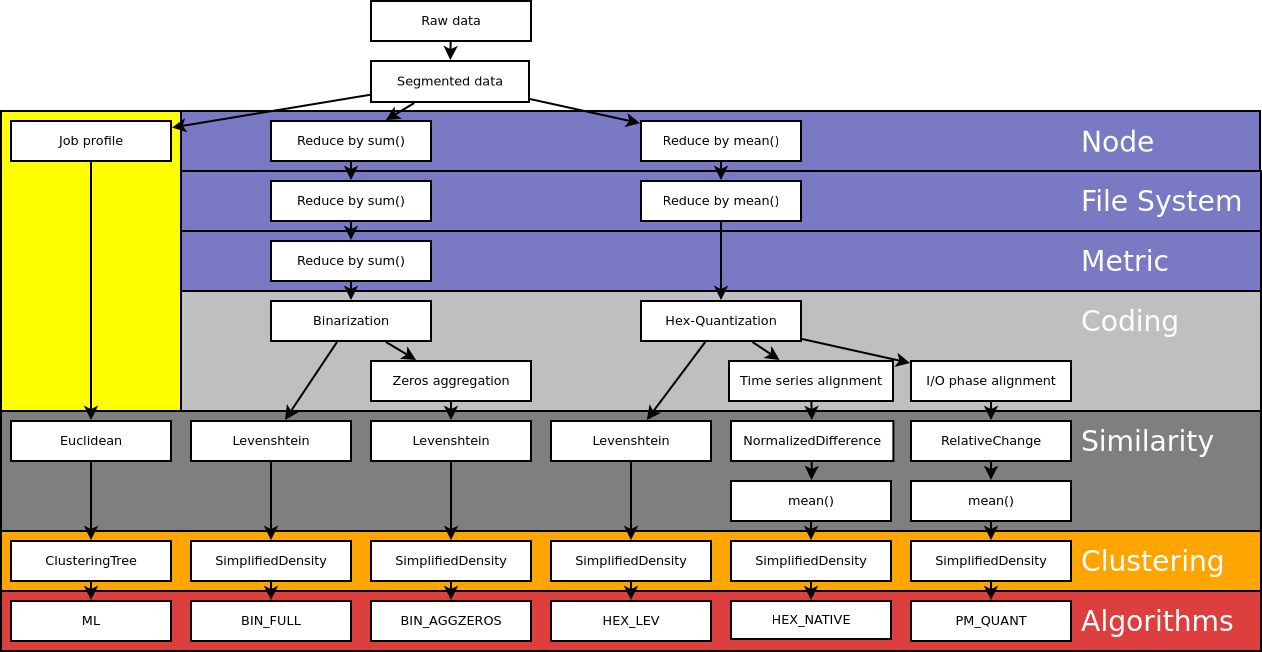
\includegraphics[width=1\textwidth]{clustering_stack.png}
  \caption{Algorithms and their actual operation stacks.}
  \label{fig:clustering_stacks}
\end{figure}


\begin{table}[ht]
  \begin{tabularx}{\textwidth}{lX}
    Algorithm & Characterization \\
    \midrule
    ML            & a set of \textbf{traditional machine learning} techniques on job profiles.                                                        \\
    BIN\_ALL      & \textbf{Levenshtein} distance applied on \textbf{binary codings.}                                                                 \\
    BIN\_AGGZEROS & \textbf{Levenshtein} distance applied on \textbf{binary codings}, but with \textbf{zero aggregation} of contiguous zero segments. \\
    HEX\_LEV      & \textbf{Levenshtein} distance applied on \textbf{hexadecimal coding}.                                                             \\
    HEX\_NATIVE   & A \textbf{performance-aware} algorithm operating on hexadecimal coding.                                                                                           \\
    PM\_QUANT     & A \textbf{performance-aware} and \textbf{I/O phase-aware} algorithm.                                                              \\
  \end{tabularx}
  \caption{Algorithm characterization}
  \label{tab:alg_character}
\end{table}

%\begin{itemize}
% \item (ML): a set of \textbf{traditional machine learning} techniques on job profiles.
% \item (BIN\_ALL): \textbf{Levenshtein} distance applied on \textbf{binary codings.}
% \item (BIN\_AGGZEROS):  \textbf{Levenshtein} distance applied on \textbf{binary codings}, but with \textbf{zero aggregation} of contiguous zero segments.
% \item (HEX\_LEV): \textbf{Levenshtein} distance applied on \textbf{hexadecimal coding}.
% \item (HEX\_NATIVE): a \textbf{performance-aware} algorithm.
% \item (PM\_QUANT): a \textbf{performance-aware} and \textbf{I/O phase-aware} algorithm.
%\end{itemize}


\subsection{Algorithms}
This section describes the evaluated algorithms in detail.

\subsubsection{ML}

To apply existing clustering algorithms, first, a job-profile is created in the pre-processing.
The 4d time series can be transformed into the required fixed-size input format accepted by the general-purpose ML clustering algorithms.
In the pre-processing step, the MinMaxScaler scales the features to values between 0 and 1 using MinMax normalization.
The Eucledian distance is used; therefore, the highest distance between two points can be at most \(\epsilon_\text{max} = d^{1/d}\), where d is the dimension of the dataset.

We explored two job profiles: IO-metric and I/O-duration.
The \textbf{IO-metric job profile} utilizes three features, Job-I/O-Balance, Job-I/O-Utilization, and Job-I/O-Problem-Time (as defined in \cite{iocats2020}).
After the data pre-processing, we obtain a set of 3-dimensional data points with a domain between 0 and 1.
The maximum distance between any two jobs ($\epsilon_{max}$) is 1.44.

The \textbf{IO-duration job profile} contains the fraction of runtime, a job spent doing the individual I/O categories leading to 27 columns.
The columns are named according to the following scheme: metric\_category, e.g, bytes\_read\_0 or md\_file\_delete\_4.
The first part is the one of the nine metric names and the second part is the category number (LowIO=0, HighIO=1 and CriticalIO=4).
These columns are used for machine learning as input features.
There is a constraint for each metric (metric\_0 + metric\_1 + metric\_4 = 1), that makes 9 features redundant, because they can be computed from the other features.
So we have to deal with 18 features; $\epsilon_{max}$ is 1.17.

\paragraph{Clustering algorithm}
%We apply agglomerative clustering.
%\jk{Könnte noch bissl unklar sein}
We found that the size of our datasets is the first obstacle to the suitable clustering algorithms.
For example, the scaling behavior of the agglomerative clustering algorithm that is used in this work can handle around 10,000 jobs in a reasonable amount of time as the complexity is $O(N^{2})$.

The agglomerative clustering algorithm uses Euclidean distance as a similarity measure, i.e., if the component wise distance between two job vectors is shorter than the defined distance ($\epsilon$), then these jobs belong to the same cluster.

Therefore, to be able to cluster 1,000,000 samples, we created a variant of the algorithm by utilizing a decision tree.
This workaround involves three steps:

\begin{enumerate}
 \item Cluster and label 10,000 jobs with the agglomerative clustering algorithm
 \item Train a decision tree model with data from the previous step
 \item Predict labels of 1,000,000 jobs with the trained decision tree model
\end{enumerate}

\subsubsection{BIN\_ALL}
This algorithm converts the time series data via binary coding to a string and then determine the relative similarity using the Levenshtein distance.
The Levenshtein based similarity between two jobs is determined using \Cref{eq:sim:bin_all}.

\begin{equation}
	\text{similarity}\left(\text{job}_{A},\text{job}_{B} \right) = 1 - \frac{\text{levenshtein}\left(\text{job}_{A},\text{job}_{B} \right) }{\max \left(|job_{A}|,|job_{B}| \right) } \label{eq:sim:bin_all}
\end{equation}
It is the number of Levenshtein operations (changes/deletes/inserts) divided by the length of the longest sequence, and subtracted from the value one.

%\begin{lstlisting}[caption={The similarity between these two jobs is 73 percent.}]
%'jobid': 'jobA', 'coding': [1:5:0:0:0:0:0:0:96:96:96:96:96:96:96], 'length': 15
%'jobid': 'jobB', 'coding': [0:0:0:0:0:0:0:0:0:96:96:96:96:96:98], 'length': 15
%\end{lstlisting}

\begin{listing}
	\noindent\begin{minipage}{0.50\textwidth}
		\begin{lstlisting}
		[1:5:0:0:0:0:0:96:96:96:96:96:96:96]
		\end{lstlisting}
		\vspace{-2em}
		\subcaption{Job A}
		\label{lst:test:a}
	\end{minipage}
	\hfill
	\noindent\begin{minipage}{0.50\textwidth}
		\begin{lstlisting}
		[0:0:0:0:0:0:0:0:96:96:96:96:96:98]
		\end{lstlisting}
		\vspace{-2em}
		\subcaption{Job B}
		\label{lst:test:b}
	\end{minipage}
	\caption{BIN\_ALL: The similarity between these two jobs is 73 percent}
	\label{lst:test}
\end{listing}


\subsubsection{BIN\_AGGZEROS}
This is a variant of BIN\_ALL where subsequent zero-sequences are reduced to a single zero segment before \Cref{eq:sim:bin_aggzeros} is applied.
This allows us to focus on I/O intensive parts of the job.
The example below shows the reduced codings from the previous example.

\begin{equation}
	\text{similarity} \left(\text{job}_{A},\text{job}_{B} \right) =1- \frac{\text{levenshtein} \left(\text{job}_{A},\text{job}_{B} \right) }{\max \left( |job_{A}|,|job_{B}| \right) } \label{eq:sim:bin_aggzeros}
\end{equation}

%\begin{lstlisting}[caption={The similarity between these two jbos is 53 percent.}]
%\begin{lstlisting}[caption={The two previous jobs are now encoded slightly different leading to a similarity of 53 percent.}]
%'jobid': 'jobA', 'coding': [1:5:0:96:96:96:96:96:96:96], 'length': 15
%'jobid': 'jobB', 'coding': [0:96:96:96:96:96:98], 'length': 15
%\end{lstlisting}

\begin{listing}
	\noindent\begin{minipage}{0.49\textwidth}
		\begin{lstlisting}
		[1:5:0:96:96:96:96:96:96:96]
		\end{lstlisting}
		\vspace{-2em}
		\subcaption{Job A}
		\label{lst:sim:bin_aggzeros:job_a}
	\end{minipage}
	\noindent\begin{minipage}{0.49\textwidth}
		\begin{lstlisting}
		[0:96:96:96:96:96:98]
		\end{lstlisting}
		\vspace{-2em}
		\subcaption{Job B}
		\label{lst:sim:bin_aggzeros:job_b}
	\end{minipage}
	\caption{BIN\_AGGZEROS: The similarity between these two jobs is 53 percent}
	\label{lst:sim:bin_aggzeros}
\end{listing}

\subsubsection{HEX\_LEV}
This algorithm works on the same principle as the BIN algorithms, with the difference that it applies a hexadecimal coding and then computes the mean similarity across all metrics using Levenshtein.
This adaption allows a comparison of time series where one metrics differs as only one metric string would differ while with binary coding the overall string would be different.

\begin{equation}
	\text{similarity}\left(\text{job}_{A},\text{job}_{B} \right) = 1 - \frac{ \sum_{m \in Metrics}^{} \text{levenshtein} \left(\text{job}_{A,m},\text{\text{job}}_{B,m} \right) }{|\text{Metrics}| \cdot \max(|job_A|, |job_{B}|)}
\end{equation}

\subsubsection{HEX\_NATIVE}
This algorithm computes a performance-aware similarity between two jobs.
It works with a selection of I/O intensive metrics from hexadecimal codings ($\text{Metrics}_{\text{IO}}$) and utilizes the Normalized-Difference distance for similarity computation.
%It utilizes only the I/O intensive metrics, denoted by $\text{Metrics}_{\text{IO}}$.
%This set contains those metrics where at least one job contains at least one non-zero segment in this metric.
Assume there are two jobs, $job_A$ and $job_B$.
I/O intensive metrics are those, which have either in $job_A$ or in $job_B$ at least one non-zero segment.
Further, assume $job_B$ is larger or equal than $job_A$.
Then the job similarity between the two jobs can be computed using \Cref{eq:hexn}.

%\begin{multline}
%  \text{similarity}\left(\text{job}_{A},\text{job}_{B} \right) = \frac{1}{|M_{IO}|} \sum_{m \in M_{IO}}^{} {\text{maxSimilarity} \left( \text{job}_{A,m}, \text{job}_{B,m} \right)}
%  \text{ , with }L_{B} \geq L_{A} \label{eq:hexn}
%\end{multline}
\begin{equation}
  \text{similarity}\left(\text{job}_{A},\text{job}_{B} \right) = \frac{ \sum_{m \in \text{Metrics}_{\text{IO}}}^{} {\text{maxSimilarity} \left( \text{job}_{A,m}, \text{job}_{B,m} \right)}}{|\text{Metrics}_{\text{IO}}|}
  \label{eq:hexn}
\end{equation}

The algorithm assumes that the metric codings $job_{B,m}$ and $job_{A,m}$ can be of different lengths.
Therefore, to compute similarity, it trims the most irrelevant segments of the longer time series, which are determined by the sliding window approach, with the goal to find maximum similarity between two metrics.
That means, we take the shortest coding sequence (CA) and check how it fits best on the longer coding sequence (CB).
The best fitted slice is denoted as (SB).

\begin{lstlisting}[caption={Pseudo code of the maxSimilarity() function}]
float maxSimilarity(CA, CB) {
  max = 0
  LA = length(CA)
  LB = length(CB)
  for pos in 0..(LB-LA) { // LB-LA is the boundary, as stated: LB > LA
    SB = substr(str=CB, start=pos, len=LA)
    sim = sliceSimilarity(CA, SB)
    if sim > max {
      max = sim
    }
  }
  return max
}
\end{lstlisting}

The \texttt{sliceSimilarity()} in \Cref{eq:slicesim} computes similarity between two codings of the same length.
It iterates over all positions of the coding $C_A$ and slice $S_B$, computes segment similarities, and the sum.
Lastly, it normalizes the sum by the length of $job_B$.
This function maps the differences between performance levels of the same segments (values between 0 and 16) to a relative value between 0 and 1.

\begin{equation}
	\text{sliceSimilarity}\left(C_{A},S_{B}\right) = \frac{1}{|job_B|}\sum_{\text{pos}=1}^{|job_A|} \left(1 - \frac{\vert C_{A,\text{pos}}-S_{B,\text{pos}} \vert }{16}\right)\text{, with }|job_{B}| \geq |job_{A}| \label{eq:slicesim}
\end{equation}

In \Cref{lst:sim:hex_native} we apply the approach to compute similarity between two jobs; the trimmed metrics are shown only to highlight similarity and difference between the jobs better.
First, we determine and trim the I/O intensive metrics in \Cref{lst:sim:hex_native:job_a:mio,lst:sim:hex_native:job_b:mio}.
Then we use the \Cref{eq:slicesim} to computed individual metrics similarities, and finally, we compute the mean in \Cref{tab:hex_native:compute_sim}.
According to this algorithm, the two jobs in the table are similar to 73\% as 7 of the metrics are actually identical.

\begin{listing}
	\noindent\begin{minipage}{\textwidth}
		\noindent\begin{minipage}{0.6\textwidth}
			\begin{lstlisting}[basicstyle=\fontsize{8}{8}\ttfamily]
			md_file_create [0:0:0:0]
			md_file_delete [0:0:0:0]
			md_mod         [0:0:0:0]
			md_other       [0:0:0:0]
			md_read        [1:1:0:0]
			read_bytes     [1:1:2:2]
			read_calls     [0:0:0:0]
			write_bytes    [0:0:0:0]
			write_calls    [0:0:0:0]
			\end{lstlisting}
			\vspace{-2em}
			\subcaption{Coding of Job A}
			\label{lst:sim:hex_hative:job_a}
		\end{minipage}
		\noindent\begin{minipage}{0.39\textwidth}
			\begin{lstlisting}[basicstyle=\fontsize{8}{8}\ttfamily]
			[]
			[]
			[]
			[]
			[1:1:0:0]
			[1:1:2:2]
			[]
			[0:0:0:0]
			[]
			\end{lstlisting}
			\vspace{-2em}
			\subcaption{Metrics of Job A}
			\label{lst:sim:hex_native:job_a:mio}
		\end{minipage}
	\end{minipage}

	\noindent\begin{minipage}{\textwidth}
		\noindent\begin{minipage}{0.60\textwidth}
		\begin{lstlisting}[basicstyle=\fontsize{8}{8}\ttfamily]
		md_file_create [0:0:0:0:0]
		md_file_delete [0:0:0:0:0]
		md_mod         [0:0:0:0:0]
		md_other       [0:0:0:0:0]
		md_read        [5:5:0:0:0]
		read_bytes     [1:1:1:2:2]
		read_calls     [0:0:0:0:0]
		write_bytes    [0:0:4:8:0]
		write_calls    [0:0:0:0:0]
		\end{lstlisting}
		\vspace{-2em}
		\subcaption{Coding of Job B}
		\label{lst:sim:hex_native:job_b}
		\end{minipage}
		\noindent\begin{minipage}{0.39\textwidth}
			\begin{lstlisting}[basicstyle=\fontsize{8}{8}\ttfamily]
			[]
			[]
			[]
			[]
			[5:5:0:0]
			[1:1:2:2]
			[]
			[0:0:4:8]
			[]
			\end{lstlisting}
			\vspace{-2em}
			\subcaption{Trimmed metrics of Job B}
			\label{lst:sim:hex_native:job_b:mio}
		\end{minipage}
	\end{minipage}
	\caption{HEX\_NATIVE: Hexadecimal codings of two jobs and I/O intensive metrics.}
	\label{lst:sim:hex_native}
\end{listing}

\begin{listing}
		\noindent\begin{minipage}{0.49\textwidth}
			\begin{lstlisting}[basicstyle=\fontsize{8}{8}\ttfamily]
			md_file_create [0:0:0:0]
			md_file_delete [0:0:0:0]
			md_mod         [0:0:0:0]
			md_other       [0:0:0:0]
			md_read        [1:1:0:0]
			read_bytes     [1:1:2:2]
			read_calls     [0:0:0:0]
			write_bytes    [0:0:0:0]
			write_calls    [0:0:0:0]
			\end{lstlisting}
			\vspace{-2em}
			\subcaption{Coding of Job A}
			\label{lst:sim:hex_hative:step1:job_a}
		\end{minipage}
		\noindent\begin{minipage}{0.49\textwidth}
		\begin{lstlisting}[basicstyle=\fontsize{8}{8}\ttfamily]
		md_file_create [0:0:0:0:0]
		md_file_delete [0:0:0:0:0]
		md_mod         [0:0:0:0:0]
		md_other       [0:0:0:0:0]
		md_read        [5:5:0:0:0]
		read_bytes     [1:1:1:2:2]
		read_calls     [0:0:0:0:0]
		write_bytes    [0:0:4:8:0]
		write_calls    [0:0:0:0:0]
		\end{lstlisting}
		\vspace{-2em}
		\subcaption{Coding of Job B}
		\label{lst:sim:hex_native:step1:job_b}
		\end{minipage}
	\caption{HEX\_NATIVE: Hexadecimal codings of two jobs and I/O intensive metrics.}
	\label{lst:sim:hex_native:step1}
\end{listing}

\begin{listing}
		\noindent\begin{minipage}{0.49\textwidth}
			\begin{lstlisting}[basicstyle=\fontsize{8}{8}\ttfamily]
			md_file_create [0:0:0:0]
			md_file_delete [0:0:0:0]
			md_mod         [0:0:0:0]
			md_other       [0:0:0:0]
			md_read        [1:1:0:0]
			read_bytes     [1:1:2:2]
			read_calls     [0:0:0:0]
			write_bytes    [0:0:0:0]
			write_calls    [0:0:0:0]
			\end{lstlisting}
			\vspace{-2em}
			\subcaption{Coding of Job A}
			%\label{lst:sim:hex_hative:step1:job_a}
		\end{minipage}
		\noindent\begin{minipage}{0.49\textwidth}
		\begin{lstlisting}[basicstyle=\fontsize{8}{8}\ttfamily]
		md_file_create [0:0:0:0:0]
		md_file_delete [0:0:0:0:0]
		md_mod         [0:0:0:0:0]
		md_other       [0:0:0:0:0]
		md_read        [5:5:0:0:0]
		read_bytes     [1:1:1:2:2]
		read_calls     [0:0:0:0:0]
		write_bytes    [0:0:4:8:0]
		write_calls    [0:0:0:0:0]
		\end{lstlisting}
		\vspace{-2em}
		\subcaption{Coding of Job B}
		%\label{lst:sim:hex_native:step1:job_b}
		\end{minipage}
	\caption{HEX\_NATIVE: Hexadecimal codings of two jobs and I/O intensive metrics.}
	%\label{lst:sim:hex_native:step1}
\end{listing}



\begin{table}[t]
\centering
\begin{tabular}{lllr}
 	$\text{Metric}_{IO}$ & $C_A$                 & $C_B$                   \\ 
 	\midrule
 	md\_read             & \lstinline|[1:1:0:0]| & \lstinline|[5:5:0:0:0]| \\ 
 	read\_bytes          & \lstinline|[1:1:2:2]| & \lstinline|[1:1:1:2:2]| \\ 
 	write\_bytes         & \lstinline|[0:0:0:0]| & \lstinline|[0:0:4:8:0]| \\ 
 	\midrule
 	Mean                 &                       &                         \\ 
\end{tabular}
\caption{HEX\_NATIVE: Similarity computation.}
%\label{tab:hex_native:compute_sim}
\end{table}

%1 5 -> 0.75
%1 5 -> 0.75
%0 0 -> 1
%0 0 -> 1
%Sum 3.5
%SliceSimilarity 0.7
%1 5 -> 0.75
%1 0 -> 0.9375
%0 0 -> 1
%0 0 -> 1
%Sum 3.6875
%SliceSimilarity 0.7375
%Final SliceSimilarity 0.7375
%1 1 -> 1
%1 1 -> 1
%2 1 -> 0.9375
%2 2 -> 1
%Sum 3.9375
%SliceSimilarity 0.7875
%1 1 -> 1
%1 1 -> 1
%2 2 -> 1
%2 2 -> 1
%Sum 4
%SliceSimilarity 0.8
%Final SliceSimilarity 0.8
%0 0 -> 1
%0 0 -> 1
%0 4 -> 0.75
%0 8 -> 0.5
%Sum 3.25
%SliceSimilarity 0.65
%0 0 -> 1
%0 4 -> 0.75
%0 8 -> 0.5
%0 0 -> 1
%Sum 3.25
%SliceSimilarity 0.65
%Final SliceSimilarity 0.65
%sim 0.7291667


\begin{table}[t]
\centering
\begin{tabular}{lllrr}
  $\text{Metric}_{IO}$       & $C_A$                 & $S_B$                 & SliceSimilarity($C_A$, $S_B$) \\ 
  \midrule
  md\_read     & \lstinline|[1:1:0:0]| & \lstinline|[5:5:0:0]| & 0.7                           \\ 
  &                       & \lstinline|[5:0:0:0]| & \textbf{0.7375}                        \\ 
  read\_bytes  & \lstinline|[1:1:2:2]| & \lstinline|[1:1:1:2]| & 0.7875                        \\ 
  &                       & \lstinline|[1:1:2:2]| & \textbf{0.8}                         \\ 
  write\_bytes & \lstinline|[0:0:0:0]| & \lstinline|[0:0:4:8]| & 0.65                          \\ 
               &                       & \lstinline|[0:4:8:0]| & 0.65                          \\ 
  \midrule
  Mean         &                       &                       & $\approx$0.73                 \\ 
\end{tabular}
\caption{HEX\_NATIVE: Similarity computation.}
\label{tab:hex_native:compute_sim}
\end{table}


\subsubsection{PM\_QUANT}
The developed phase-matching quantization algorithm allows us to cluster variable length jobs by aligning IO phases.
First, using a hexadecimal coding, phases of consecutive I/O segments are detected and extracted.
Then, the best match between the (disjoint) phases is determined, finally the similarity is computed.
We will discuss the details of each step on the example jobs in \Cref{lst:sim:pm_quant}.


\begin{listing}
	\noindent\begin{minipage}{\textwidth}
		\noindent\begin{minipage}{0.6\textwidth}
			\begin{lstlisting}[basicstyle=\fontsize{8}{8}\ttfamily]
			md_file_create [0:0:2:2:2:9:3:0:9:1:1:1:0]
			md_file_delete [0:0:0:0:0:0:0:0:0:0:0:0:0]
			md_mod         [0:0:0:0:0:0:0:0:0:0:0:0:0]
			md_other       [0:0:0:0:0:0:0:0:0:0:0:0:0]
			md_read        [0:0:0:0:0:0:0:0:0:0:0:0:0]
			read_bytes     [0:0:0:9:3:0:0:0:0:0:1:0:0]
			read_calls     [0:0:0:0:0:0:0:0:0:0:0:0:0]
			write_bytes    [0:0:0:0:0:0:0:0:0:0:0:0:0]
			write_calls    [0:0:0:0:0:0:0:0:0:0:0:0:0]
			\end{lstlisting}
			\vspace{-2em}
			\subcaption{Coding of Job A}
			\label{lst:sim:pm_quant:job_a}
		\end{minipage}
		\noindent\begin{minipage}{0.39\textwidth}
			\begin{lstlisting}[basicstyle=\fontsize{8}{8}\ttfamily]
			[[2,2,2,9,3], [9,1,1,1]]
			[]
			[]
			[]
			[]
			[[9,3], [1]]
			[]
			[]
			[]
			\end{lstlisting}
			\vspace{-2em}
			\subcaption{I/O phases of Job A}
			\label{lst:sim:pm_quant:phases:job_a}
		\end{minipage}
	\end{minipage}
	\noindent\begin{minipage}{\textwidth}
		\noindent\begin{minipage}{0.60\textwidth}
		\begin{lstlisting}[basicstyle=\fontsize{8}{8}\ttfamily]
		md_file_create [1:0:0:0:0:0:0:0:0:0:0:0:0:0:0]
		md_file_delete [0:0:0:0:0:0:0:0:0:0:0:0:0:0:0]
		md_mod         [0:0:0:0:0:0:0:0:0:0:0:0:0:0:0]
		md_other       [0:0:0:0:0:0:0:0:0:0:0:0:0:0:0]
		md_read        [0:0:0:0:0:0:0:0:0:0:0:0:0:0:0]
		read_bytes     [2:2:2:2:8:2:2:0:0:1:0:0:8:1:1]
		read_calls     [0:0:0:0:0:0:0:0:0:0:0:0:0:0:0]
		write_bytes    [0:0:0:0:0:0:0:0:0:0:0:5:0:0:0]
		write_calls    [0:0:0:0:0:0:0:0:0:0:0:0:0:0:0]
		\end{lstlisting}
		\vspace{-2em}
		\subcaption{Coding of Job B}
		\label{lst:sim:pm_quant:job_b}
		\end{minipage}
		\noindent\begin{minipage}{0.39\textwidth}
			\begin{lstlisting}[basicstyle=\fontsize{8}{8}\ttfamily]
			[[1]]
			[]
			[]
			[]
			[]
			[[2,2,2,2,8,2,2], [1], [8,1,1]]
			[]
			[[5]]
			[]
			\end{lstlisting}
			\vspace{-2em}
			\subcaption{I/O phases of Job B}
			\label{lst:sim:pm_quant:phases:job_b}
		\end{minipage}
	\end{minipage}
	\caption{PM\_QUANT: Hexadecimal codings of two jobs and their I/O phases.}
	\label{lst:sim:pm_quant}
\end{listing}



\paragraph{Phase detection}
According to our I/O phase definition, phases are separated by zeros.
This definition makes the detection of individual phases to a trivial task.
Relevant for similarity computation are only metrics that contain at least one non-zero segment.
In this example, that are the md\_file\_create, read\_bytes and write\_bytes metrics:


\paragraph{Phase matching}
Now we slide the shorter phase over the longer and compute similarity to the corresponding part such that we can find the best match.
In the example, the best match is found on position four.

\def\mpw{0.32}
\begin{listing}
	\noindent\begin{minipage}{\mpw\textwidth}
		\begin{lstlisting}
		[2:2:2:2:8:2:2]
		[9:3:-:-:-:-:-]
		similarity
		= (2/9+2/3)/7
		= 13%
		\end{lstlisting}
		\vspace{-2.5em}
		\subcaption{Shift 0 positions}
	\end{minipage}
	\hfill
	\noindent\begin{minipage}{\mpw\textwidth}
		\begin{lstlisting}
		[2:2:2:2:8:2:2]
		[-:9:3:-:-:-:-]
		similarity
		= (2/9+2/3)/7
		= 13%
		\end{lstlisting}
		\vspace{-2.5em}
		\subcaption{Shift 1 position}
	\end{minipage}
	\hfill
	\noindent\begin{minipage}{\mpw\textwidth}
		\begin{lstlisting}
		[2:2:2:2:8:2:2]
		[-:-:9:3:-:-:-]
		similarity
		= (2/9+2/3)/7
		= 13%
		\end{lstlisting}
		\vspace{-2.5em}
		\subcaption{Shift 2 positions}
	\end{minipage}

	\noindent\begin{minipage}{\mpw\textwidth}
		\begin{lstlisting}
		[2:2:2:2:8:2:2]
		[-:-:-:9:3:-:-]
		similarity
		= (2/9+3/8)/7
		= 8%
		\end{lstlisting}
		\vspace{-2.5em}
		\subcaption{Shift 3 positions}
	\end{minipage}
	\hfill
	\noindent\begin{minipage}{\mpw\textwidth}
		\begin{lstlisting}
		[2:2:2:2:8:2:2]
		[-:-:-:-:9:3:-]
		similarity
		= (8/9+2/3)/7
		= 22%
		\end{lstlisting}
		\vspace{-2.5em}
		\subcaption{Shift 4 positions}
	\end{minipage}
	\hfill
	\noindent\begin{minipage}{\mpw\textwidth}
		\begin{lstlisting}
		[2:2:2:2:8:2:2]
		[-:-:-:-:-:9:3]
		similarity
		= (2/9+2/3)/7
		= 13%
		\end{lstlisting}
		\vspace{-2.5em}
		\subcaption{Shift 5 positions}
	\end{minipage}
	\caption{Phase matching example.}
	\label{lst:pm_quant:phase_matching_example}
\end{listing}


After repeating this step for all possible combinations of I/O phases, we chose those with the pairs with the highest similarity, and computed the match between them.
I/O phases without a pair are assigned virtually to empty phases, and their match is zero.
To compute the match we divide the lowest value for each segment and sum up the values.
The example below shows the pairs of I/O phases and their matches.

\begin{table}
\centering
\begin{tabular}{lllrr}
	Metric           & I/O Phase A                 & I/O Phase B                 & Match     & Length \\
	\midrule
	md\_file\_create & \lstinline|[-:-:-:-:-]|     & \lstinline|[2:2:2:9:3]|     & 0         & 5      \\
	                 & \lstinline|[-:1:-:-]|       & \lstinline|[9:1:1:1]|       & 1         & 4      \\
	read\_bytes      & \lstinline|[2:2:2:2:8:2:2]| & \lstinline|[-:-:-:-:9:3:-]| & 8/9 + 2/3 & 7      \\
	                 & \lstinline|[1]|             & \lstinline|[1]|             & 1         & 1      \\
	                 & \lstinline|[8:1:1]|         & \lstinline|[-:-:-]|         & 0         & 3      \\
	write\_bytes     & \lstinline|[5]|             & \lstinline|[-]|             & 0         & 1      \\
	\midrule
	Sum              &                             &                             & 3.56      & 21     \\
\end{tabular}
\caption{Best combination of I/O phases, that achieves the highest possible similarity.}
\end{table}

\paragraph{Similarity}
Next, the similarity for coding with different lengths must be adjusted.
Similarity between two jobs is the sum of matches divided by the sum of lengths of the longer phases.
In this example, we get a similarity of 17$\%$:

\begin{equation}
	\text{similarity}(\text{job}_A, \text{job}_B) = \frac{\sum_{m,i}{\text{match}_{m,i}}}{\sum_{m,i}{\text{length}_{m,i}}} = \frac{3.56}{21} \approx 0.17, \text{ with } m \in \text{Metrics}, i \in \text{Phases of } m
\end{equation}


\subsection{Assessment}
Lastly, the quality of the obtained clusters must be assessed.
Overall, we will assess their suitability using quantitative metrics such as the number of generated clusters and their sizes and qualitatively by manually exploring clusters of relevant jobs.
We want to emphasize that our goal is to find similar jobs.
Depending on data, the clustering algorithms may create thousands of clusters.
Unfortunately, it is not feasible to analyze all of them qualitatively with reasonable effort and there are no tools that can assess the cluster quality automatically.

Therefore, for the assessment, we look inside clusters and inspect segment sequences of the corresponding jobs.
For the quantitative analysis, we attempted to find clusters that show the characteristic weakness of the algorithm and discuss them.
We also define \textit{cluster relevance} as a metrics that assists in determining which cluster bears the best optimization potential and, hence, could be investigated first by the support staff.

For the qualitative analysis, we start by looking into a job that is given to user support, then similar jobs need to be found.
In the same cluster, we expect the sequences to be similar.
If not, the clustering algorithm is not effective.



\section{Evaluation}%
\label{sec:evaluation}

\subsection{Test Environment}%
\label{sec:test_environment}
For the performance tests, we allocate a compute node on Mistral supercomputer.
It is equipped with 2x Intel\textsuperscript\textregistered\@ Xeon\textsuperscript\textregistered\@ CPU E5 2680 v3 @ 2.50GHz, 64GB DDR4 RAM\@.
For clustering of job profiles, we use the agglomerative clustering algorithm, decision trees, and the MinMaxScaler from the Scikit-Learn 0.22.1 library and Python 3.8.0.
For clustering of binary and hexadecimal codings we use a clustering algorithm implemented in Rust 1.42.0, and run it on a single core.


\subsection{Description of Our Data Set}
This section describes the job data extracted from Mistral, originally we gathered 1\,million jobs from a period of 203 days.
Mostly jobs are allowed to run up to 8-hours, leading to time series with up to 48 segments.
From the perspective of this work, analysis of non-I/O-intensive jobs (jobs with zero in all segments) is irrelevant, these jobs can be grouped into one class easily.
For that reason, we detect zero-jobs early and remove them from the dataset; these are about 40\% of jobs.
%Note that PM ignores such jobs by design.
%Therefore, this step wouldn't be necessary.

The number of zero-jobs is different for hexadecimal and binary mode codings.
The reason is the quantization to HEX coding which computes mean performance values for all segments and then quantizes them into NonIO + 16 levels.
Hereby, some segments can be quantized to zeros, if the mean value is lower than 0.125.
Therefore, it may happen that some jobs fall into the zero-job category, if all segments are quantized to zeros.
It can not happen in BIN coding, because it preserves all active segments.
Interestingly, it affects around 14$\%$ of jobs.
\Cref{tab:n_intensive_jobs} shows the number of jobs that are analyzed further.

\begin{table}
  \centering
  \begin{tabular}{ll}
    Algorithm & Number of I/O intensive jobs \\
    \midrule
    BIN\_$\ast$, PM\_FLOAT, HEX\_NATIVE &  583.000 \\
    HEX\_LEV, PM\_QUANT &  444.000 \\
  \end{tabular}
  \caption{Numbers of I/O-intensive jobs.}
  \label{tab:n_intensive_jobs}
\end{table}


\subsubsection{Data exploration}
I/O phases are, according to our definition, contiguous sequences of I/O-intensive segments.
The statistics of the number phases for each different metric are visualized in \Cref{fig:phases_stats}.
These histograms show for one metric how many I/O phases a job has.
Most jobs exhibit up to 5-phases in one metrics.
The metrics (md\_bytes, md\_mod, and md\_file\_delete) have the longest tail; some job use up to 22-phases, meaning that almost every other segment the value is zero or $\geq 1$.

%We suppose these  can be exploited in clustering algorithms to achieve better results.


\begin{figure}
  \centering
  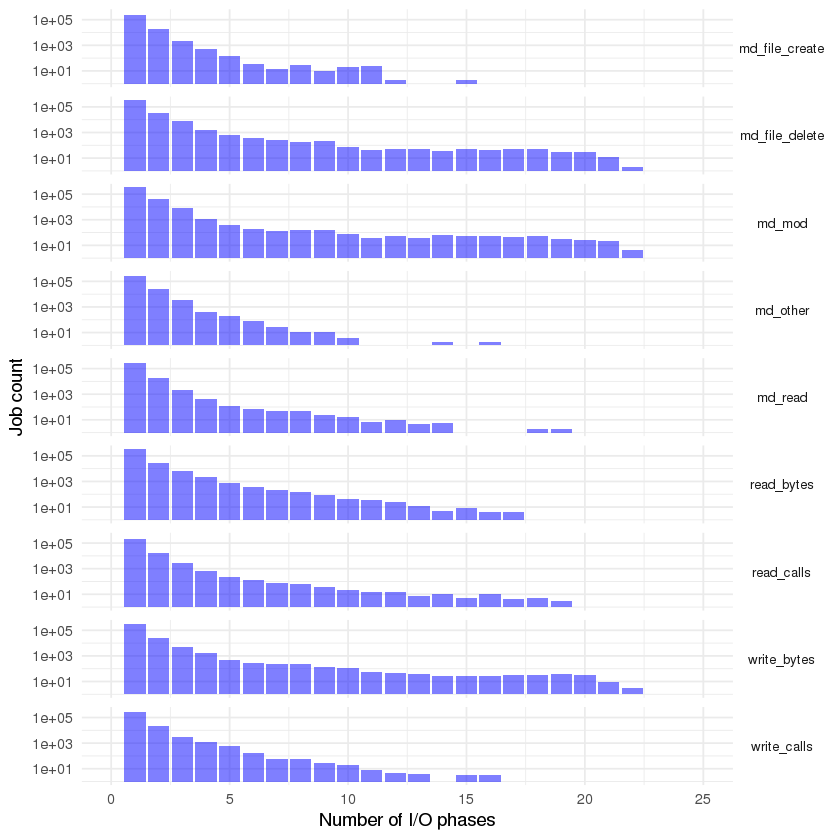
\includegraphics[width=3.55in,height=3.56in]{image23.png}
  \caption{I/O phases statistics.}
  \label{fig:phases_stats}
\end{figure}


\subsection{Explored Algorithm Parameters}
\paragraph{ML}
We explored our discussed job profiles: IO-metric and IO-duration.
For both datasets we explore $\epsilon \in [0.03, 0.06, 0.09, 0.1, 0.2, 0.3]$.

\paragraph{BIN/HEX/PM}
In the experiments with BIN*, HEX* and PM* algorithms, we cluster jobs varying the similarity parameter SIM $\in [0.1, 0.3, 0.5, 0.7, 0.9, 0.95, 0.99]$.
Additionally, we capture the clustering progress each time after clustering 10,000 jobs.


\subsection{Limitations of the ML Algorithms}
This section contains data statistics, and the clustering results in \Cref{fig:datasets_clustering_results} for applying the ML algorithm (hierarchical clustering + decision tree) but using the two different job profiles (IO-Metric and IO-Duration).
Due to lack of tools, we determine cluster quality on a small scale.

%\subsubsection{Implementation}
%The data is analyzed using Python3.8.0.
%In particular we use the agglomerative clustering algorithm, decision trees, and the MinMaxScaler from the scikit-learn 0.22.1 library.


\subsubsection{Results}
We conducted several experiments with different $\epsilon$ values between 0 and $\epsilon_{max}$.
The Top 20 largest clusters and total number of clusters is visualized in \Cref{fig:datasets_clustering_results:io_metric} and \Cref{fig:datasets_clustering_results:io_duration} for IO-metric and IO-duration job-profiles, respectively.

\begin{figure}
 \begin{subfigure}[t]{0.45\textwidth}
	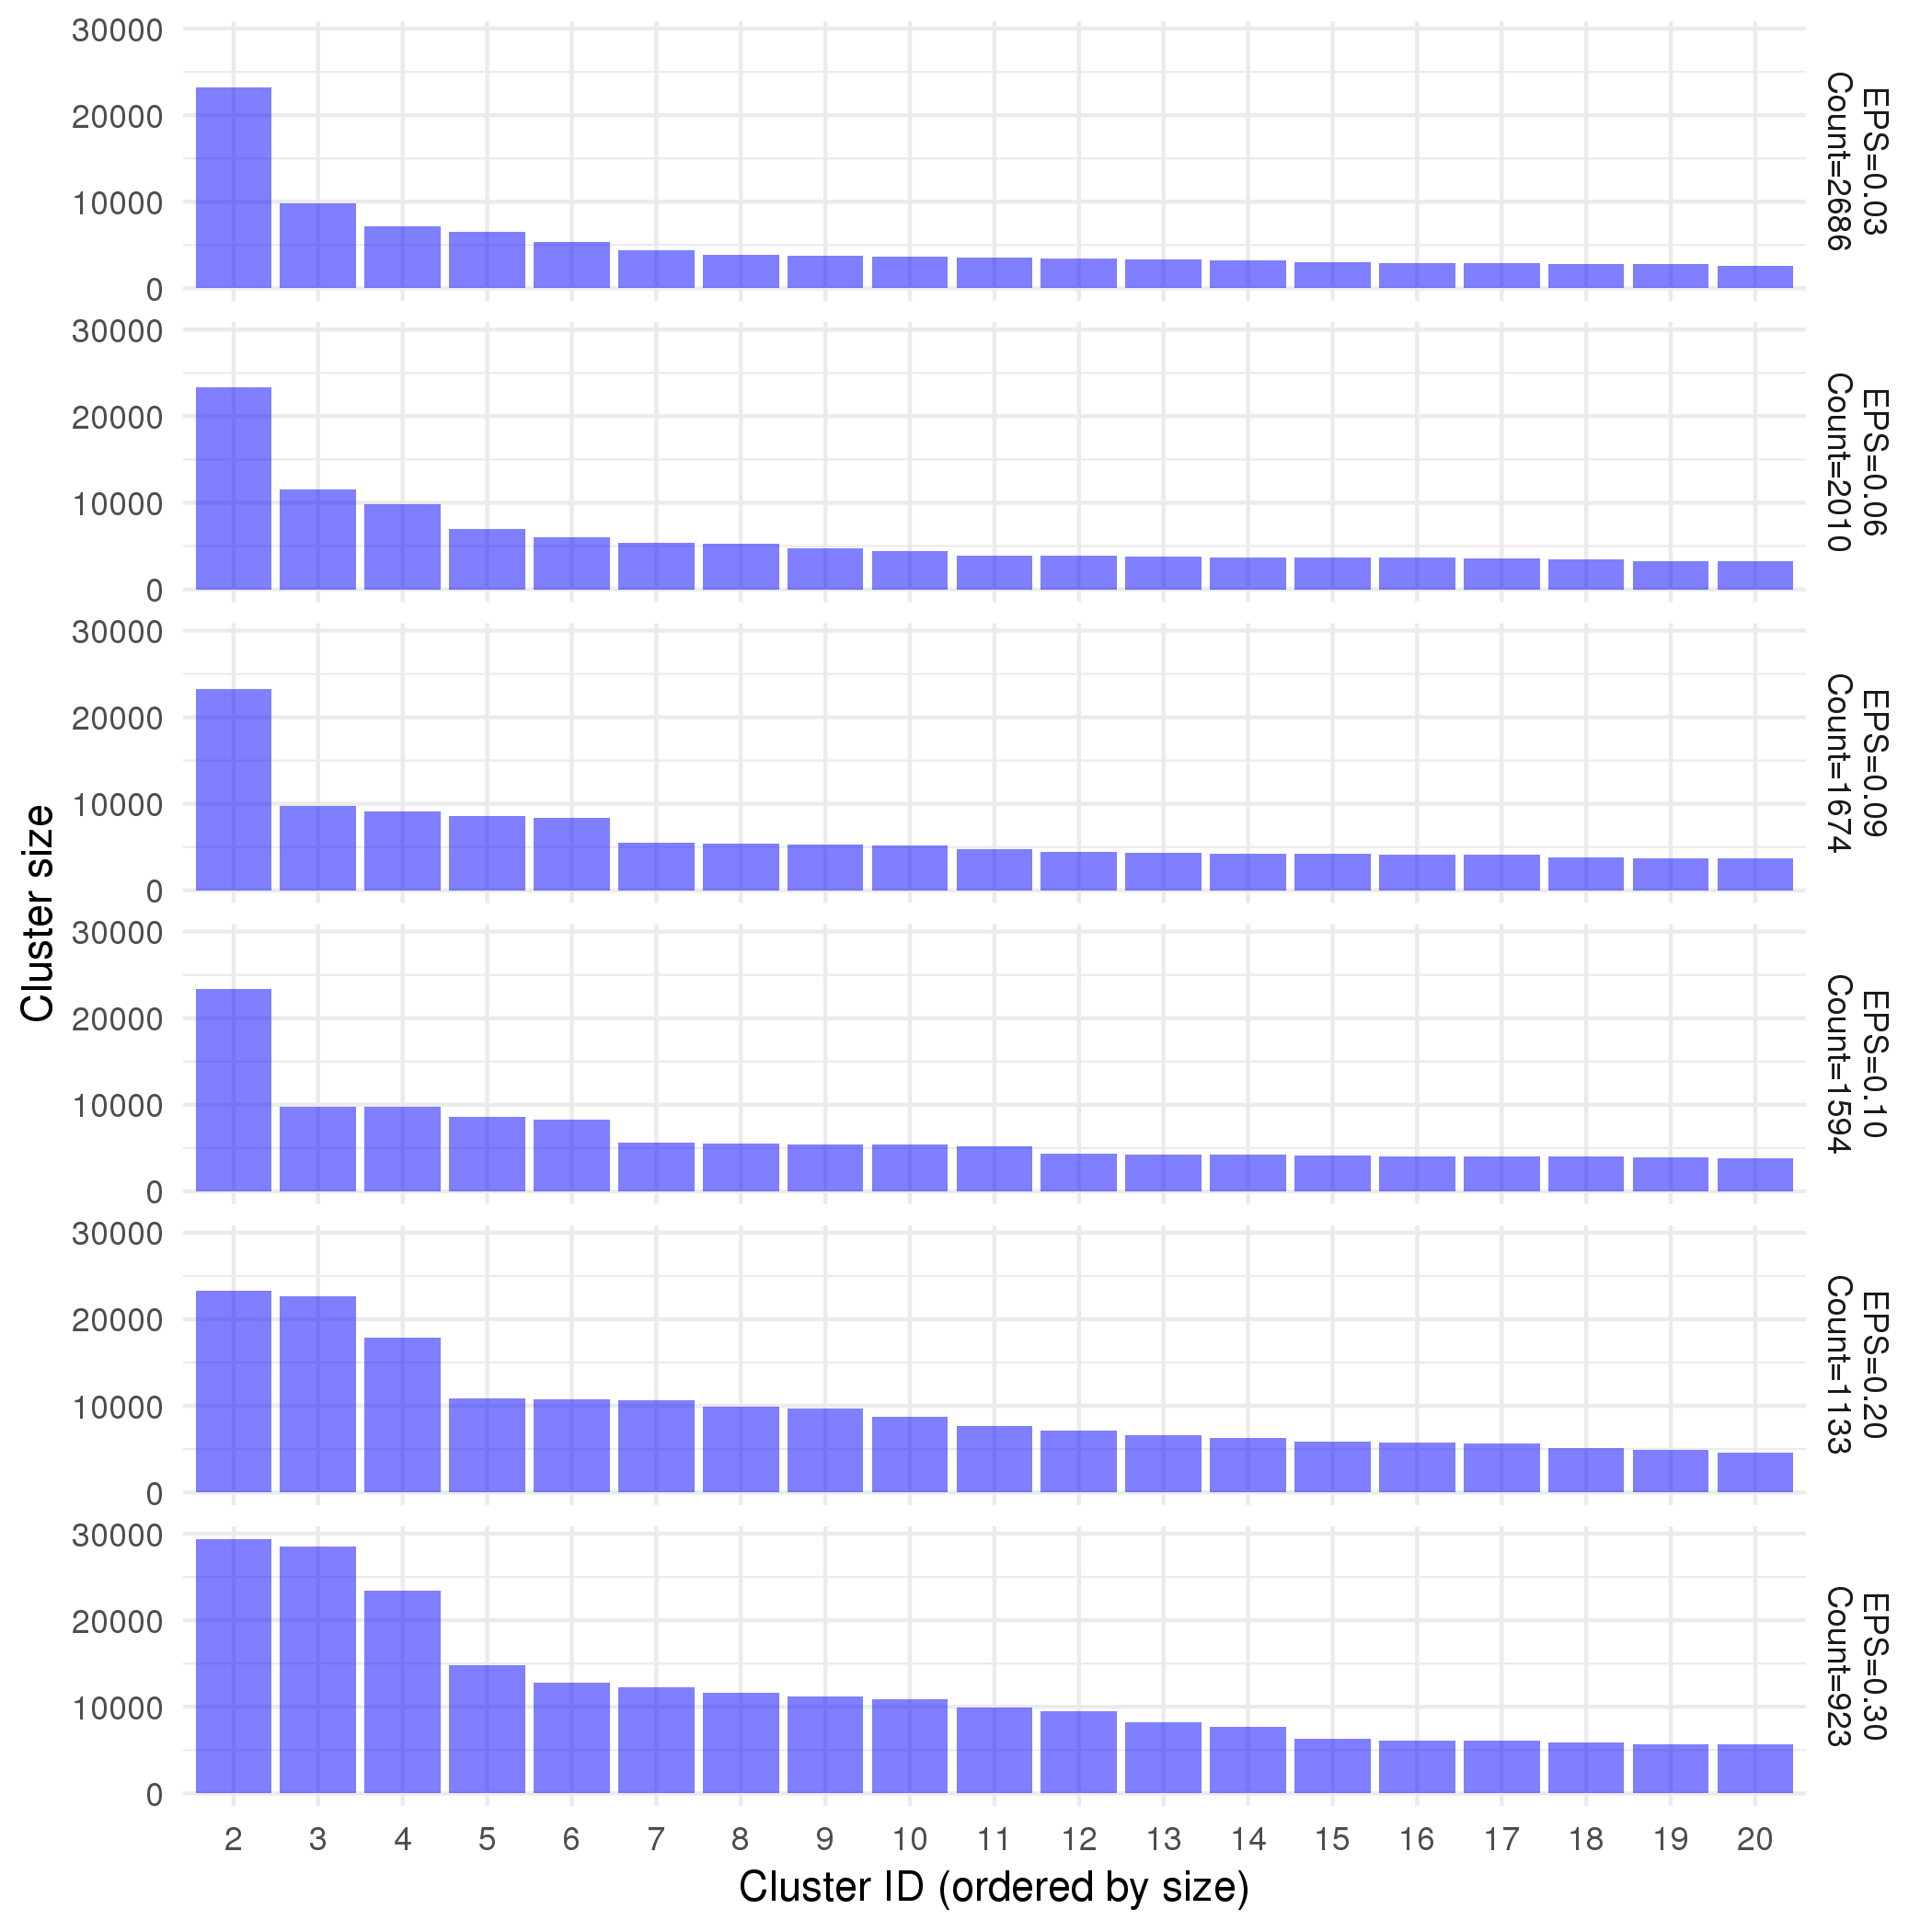
\includegraphics[width=\textwidth]{image12.png}
	\caption{IO-metric}
	\label{fig:datasets_clustering_results:io_metric}
 \end{subfigure}
 \hfill
	\begin{subfigure}[t]{0.45\textwidth}
	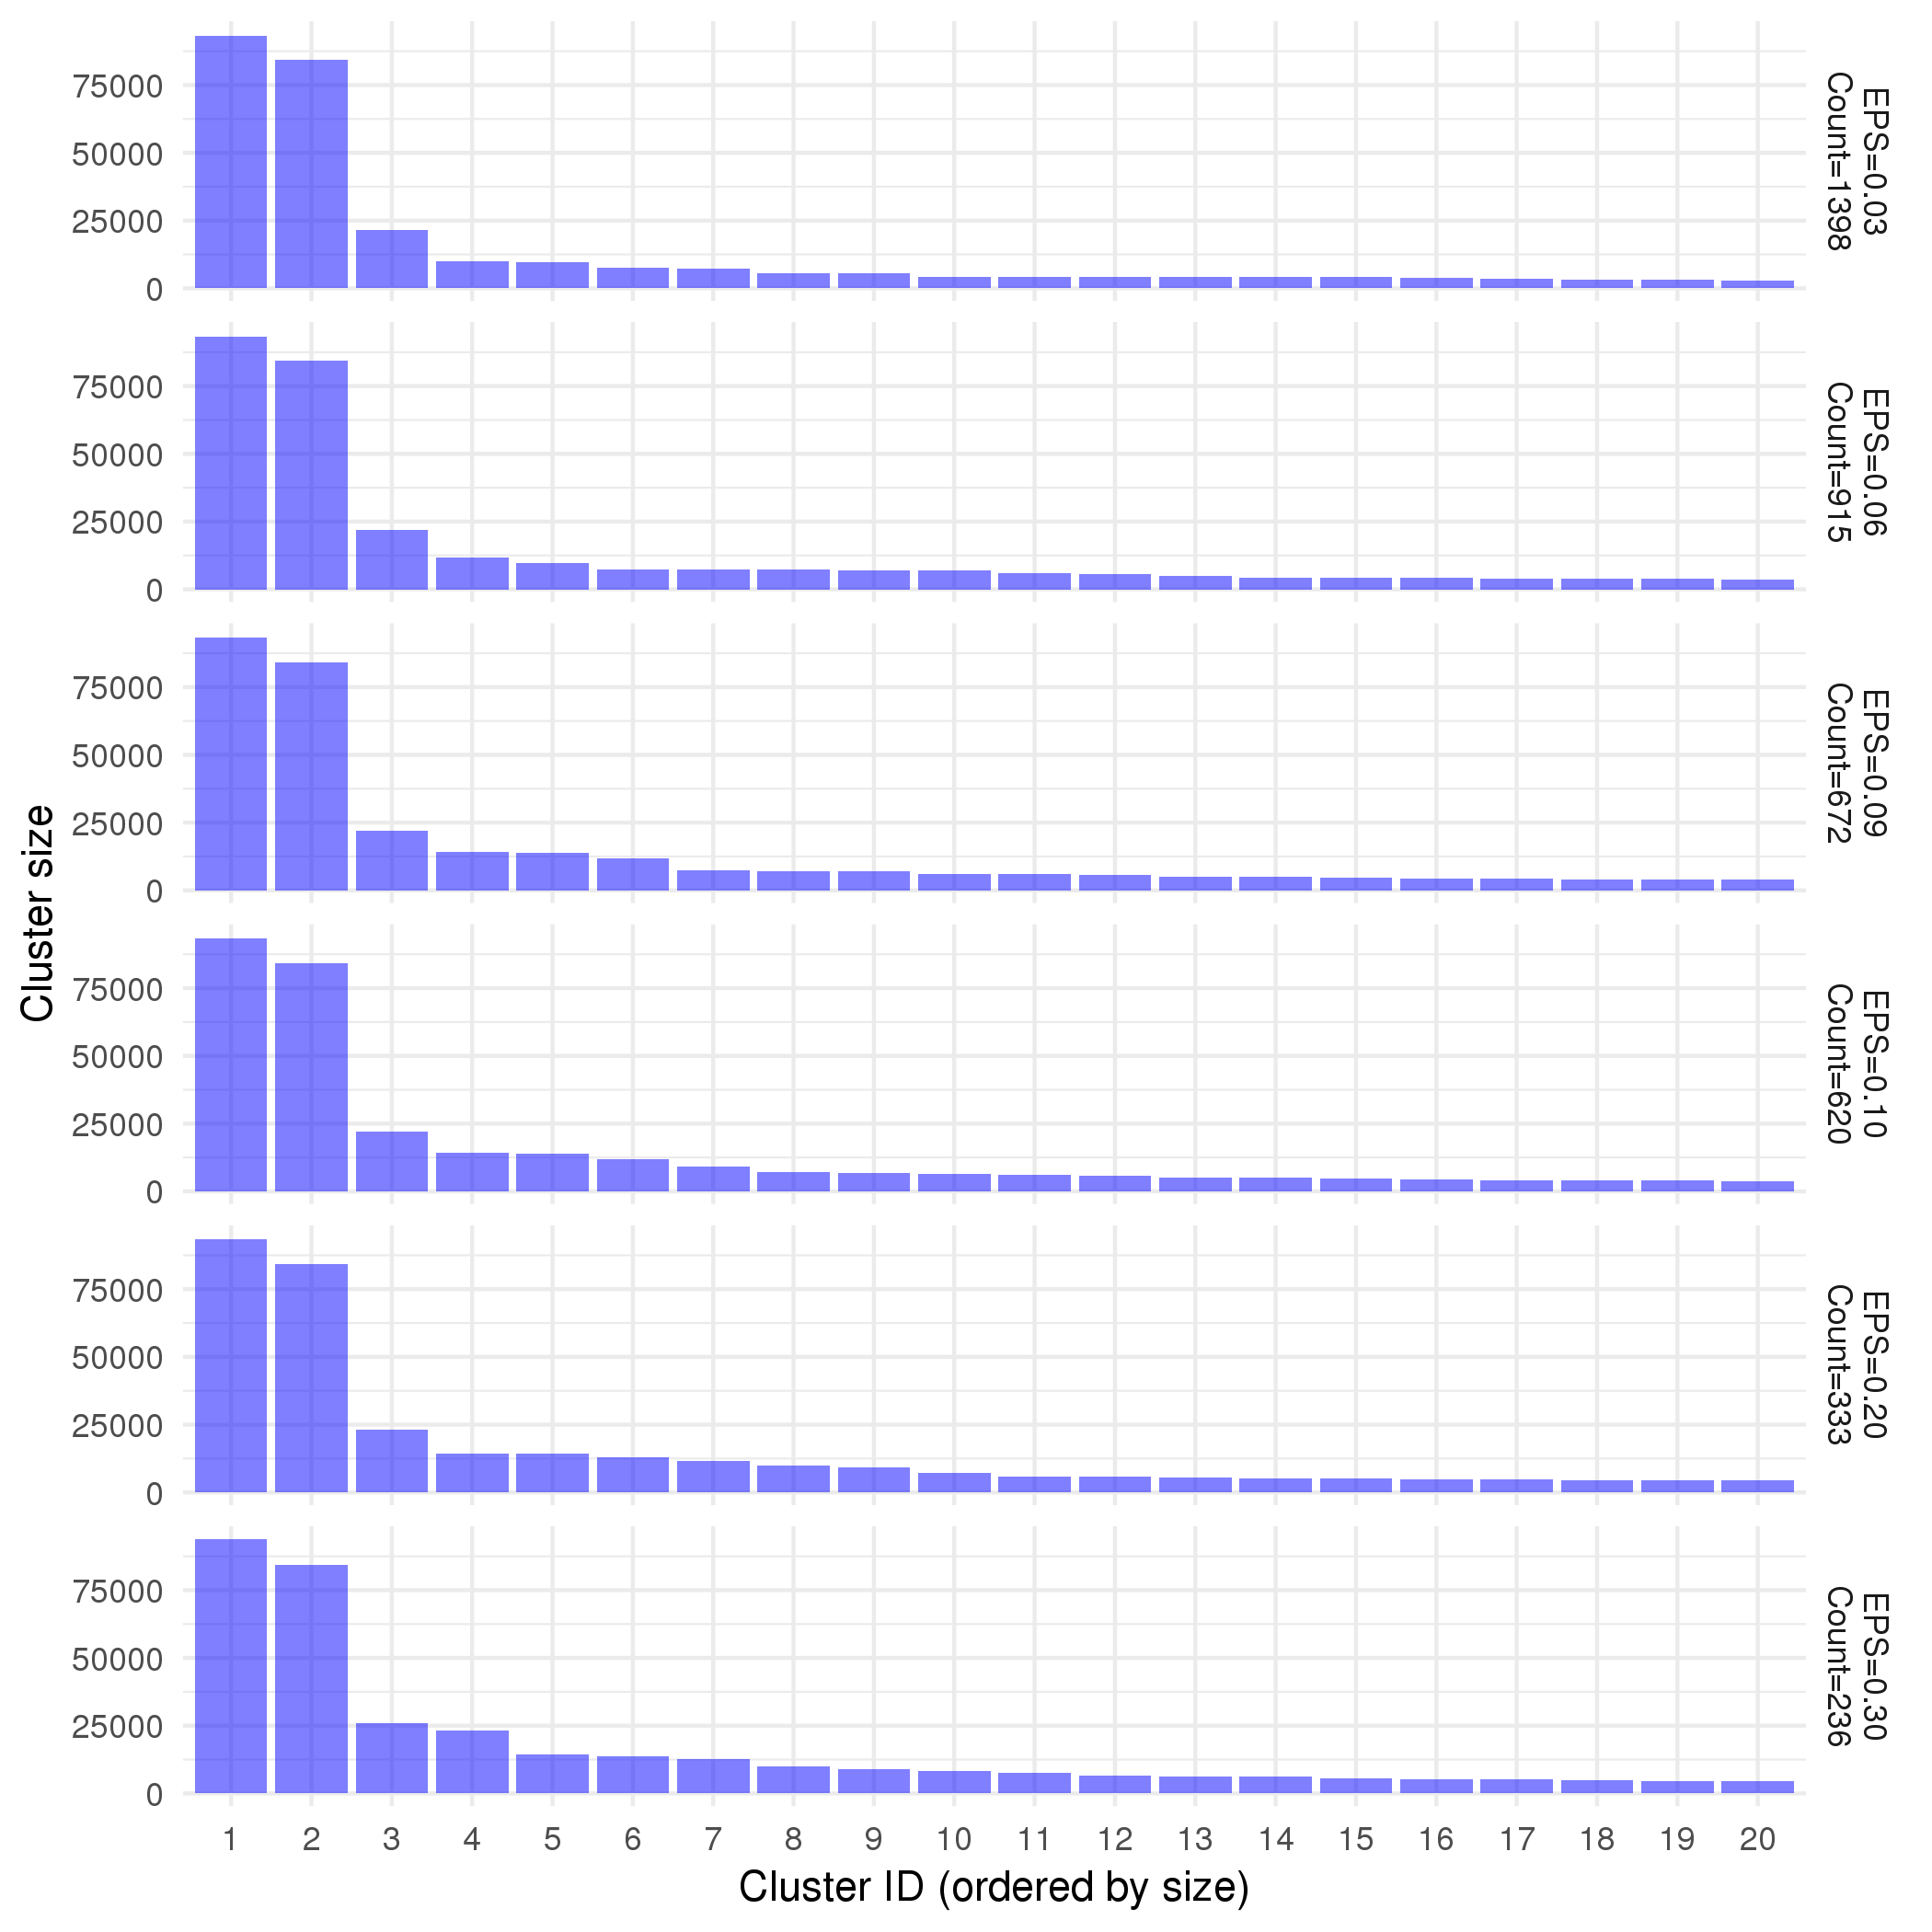
\includegraphics[width=\textwidth]{image10.png}
	\caption{IO-duration}
	\label{fig:datasets_clustering_results:io_duration}
 \end{subfigure}

 \caption{The Top 20 largest clusters for two different job-profiles.}
 \label{fig:datasets_clustering_results}
\end{figure}

We can see that IO-duration generated two very large clusters regardless of $\epsilon$.
From Cluster\,3 of IO-duration, the number of jobs inside looks then similar as for IO-metric.
In IO-metric, we can see that with increasing $\epsilon$, the number of jobs per cluster increase (as expected).

A look inside clusters reveals chaotic clustering results.
For both datasets and for all $\epsilon$ values we could find many coding sequences in a cluster that we wouldn't locate together.
As the examples in \Cref{tab:ml_examples} show, observed cluster contains the following sequences.

\npdecimalsign{.}
\nprounddigits{3}
\def\rd{3}
\newcolumntype{R}[2]{%
    >{\adjustbox{angle=#1,lap=\width-(#2)}\bgroup}%
    l%
    <{\egroup}%
}
\newcommand*\rot{\multicolumn{1}{R{45}{1em}}}% no optional argument here, please!

\begin{table}[!bt]
 \centering
 \begin{subtable}{\textwidth}
   \centering
     \begin{tabular}{lln{1}{\rd}|l}
       \rot{Job-IO-Utilization} & \rot{Job-IO-Problem-Time} & \rot{Job-IO-Balance} & \rot{Binary coding}                       \\
       \midrule
       4                        & 1                         & 0.4375000            & [118]                                     \\
       4                        & 1                         & 0.4450206            & [368:368:368:368:368:368:374:368:368:368] \\
       4                        & 1                         & 0.4583333            & [496:496]                                 \\
     \end{tabular}
   \caption{IO-metrics job profiles}
 \end{subtable}
 \begin{subtable}{\textwidth}
   \centering
     \begin{tabular}{n{1}{\rd}n{1}{\rd}n{1}{\rd}n{1}{\rd}n{1}{\rd}n{1}{\rd}n{1}{\rd}n{1}{\rd}|l}
       \rot{1\_md\_file\_delete} & \rot{1\_md\_mod} & \rot{1\_md\_other} & \rot{1\_md\_read} & \rot{1\_read\_bytes} & \rot{1\_read\_calls} & \rot{1\_write\_bytes} & \rot{1\_write\_calls} & \rot{Binary coding} \\
       \midrule
       0.009259259               & 0.01851852       & 0.25000000         & 0.027777778       & 0.00462963           & 0.009259259          & 0.00462963            & 0.03240741            & [340:510:272]       \\
       0.012578616               & 0.01257862       & 0.24528302         & 0.006289308       & 0.00617284           & 0.006172840          & 0.01257862            & 0.01257862            & [510:0:0]           \\
       0.016666667               & 0.01666667       & 0.25000000         & 0.016666667       & 0.00000000           & 0.000000000          & 0.00000000            & 0.01666667            & [14:280]            \\
     \end{tabular}
   \caption{IO-duration job profiles}
 \end{subtable}
 \caption{Jobs found in the same cluster with their profiles coding ($\epsilon = 0.03$). Columns containing zeros only are omitted.}
 \label{tab:ml_examples}
\end{table}

We looked in the Top 10 largest clusters and a random selection of clusters to find the same picture:
Even with low $\epsilon$ values the algorithms appears to produce polluted clusters, i.e, with samples from other clusters.
Like in the example above, we couldn't understand the logic behind the results.
Probably, the particular random datasets used for training does not represent the specifics of parallel jobs  well enough for proper clustering.
However, even with a good feature set that works on our test system, it is unlikely that the strategy and trained model will be portable to other systems.
Therefore, we conclude that this adapted version of hierarchical clustering based on job profiles isn't suitable to analyze the workload.

\subsection{Quantitative Evaluation}
This section contains data statistics, clustering progress, and clustering results when applying the five customized algorithms (BIN\_ALL, BIN\_AGGZEROS, HEX\_LEV, HEX\_NATIVE, PM\_QUANT).
%Due to lack of tools, we determine cluster quality on a small scale.

%\subsubsection{Implementation}
%For the performance tests we allocate a compute node on Mistral supercomputer.
%It is equipped with 2x Intel(R) Xeon(R) CPU E5-2680 v3 @ 2.50GHz, 64GB DDR4 RAM.
%The clustering algorithms are implemented in Rust and run on a single core.
%They are applied on pre-computed codings datasets, so that the clustering runtimes do not include the creation of the codings.

\subsubsection{Impact of the User-Defined Similarity}
In the introduced algorithms, the user-defined similarity (SIM) that the jobs in a cluster must fullfill to the cluster centroid controls the cluster formation.
It is expected that low SIM values produce a smaller amount of noisy clusters and a high SIM value produces a large amount of clean clusters.
We suppose the optimal value is application dependent.
Although an optimal SIM value depends on use case and dataset, a parameter exploration may provide important hints to find a good value and achieve optimal cluster qualities.

\Cref{fig:clustering_progress} shows the number of clusters created when clustering an increasing total number of jobs for different SIM values; each point represents the number for an analyzed number of jobs in increments of 10,000 jobs.
For all algorithms, we can see that with an increase in SIM value, the number of clusters created increases, and the number of total clusters created slows down the more jobs have been processed as jobs are allocated to existing clusters.
BIN creates most clusters while HEX\_NATIVE creates the least and PM is in between.
For SIM of 99\%, BIN and HEX\_LEV can barely group jobs together.


\Cref{fig:alg_runtimes} shows the clustering runtimes for the same experiment.
The clustering time depends heavily on the number of created clusters.
The reason is that the algorithm tries to put each job in existing clusters first.
It iterates over them, and only if it is not able to find a suitable cluster, it creates a new one.
The more clusters exist, the longer is the processing time.
Since, for low SIM values there is a low number of clusters, the clustering is much faster.
PM\_QUANT has exceptionally high runtimes due to quadratic runtimes of phase matching.
In one case, the runtimes clustering of 10,000 jobs took up to 4.3 hours (the few outliers are not shown in the picture).
We suppose this lies on the quadratic runtimes of the phase matching procedure.
% We didn't spend time to optimize the algorithm further.

From this initial considerations, it appears that HEX\_NATIVE is well suited, it generates the least number of clusters and is efficient.
However, looking at the overall number of created clusters isn't enough to assess the quantity of the aggregation.
Additional quantitative metrics need to be used, such as the number of small clusters.

\medskip

To understand the aggregation behavior better, alternative visualizations are investigated.
In \Cref{fig:sim_exploration}, the number of clusters created for a given similarity value is plotted.
The red line approximates the overall number of clusters, the green line shows how many contain at least two jobs and the blue line shows how many of them contain at least 10 jobs.
The maximum number of clusters is equivalent to the number of jobs; it is visualized by the gray line.
Coding with 100$\%$  similarity are of the same job phenotype, i.e, they have exactly the same length and I/O behavior.

The gradient of the curve shows the generalization capabilities of each algorithm for different SIM values.
Apparently, for all algorithms (except HEX) there is a SIM value, where the number of clusters with more than ten and two jobs is decreasing, i.e., the clustering algorithms start to split clusters into individual job clusters.
That is something we usually want to prevent, because the algorithms stop finding similar jobs, but focus on refining clusters.

\smallskip

In \Cref{fig:cum_num_job_sizes}, the distribution of the relative cluster size for all jobs.
The ABS algorithms tend to create many small clusters.
PM creates a variety of different cluster sizes and HEX\_NATIVE the biggest clusters.
Interestingly after scaling both axes with log10, we can observe a linear behavior for all algorithms.

When looking for an optimal SIM, we consider the following criteria:
Firstly, we need to select a SIM value, just before the increase of the SIM value doesn't make significant improvements.
PM and BIN algorithms work best for SIM values between 0.7 and 0.9, and for HEX the SIM value between 0.95 and 0.99.
We can also observe flattening curves with increasing numbers of jobs, which indicates that more jobs are placed in clusters and less clusters are created.
One strategy for the analysis could also be to start with a low SIM value and then increase it further to "hierarchically" cluster jobs and filter jobs that appear irrelevant for the current analysis.

\begin{figure}
  \centering
   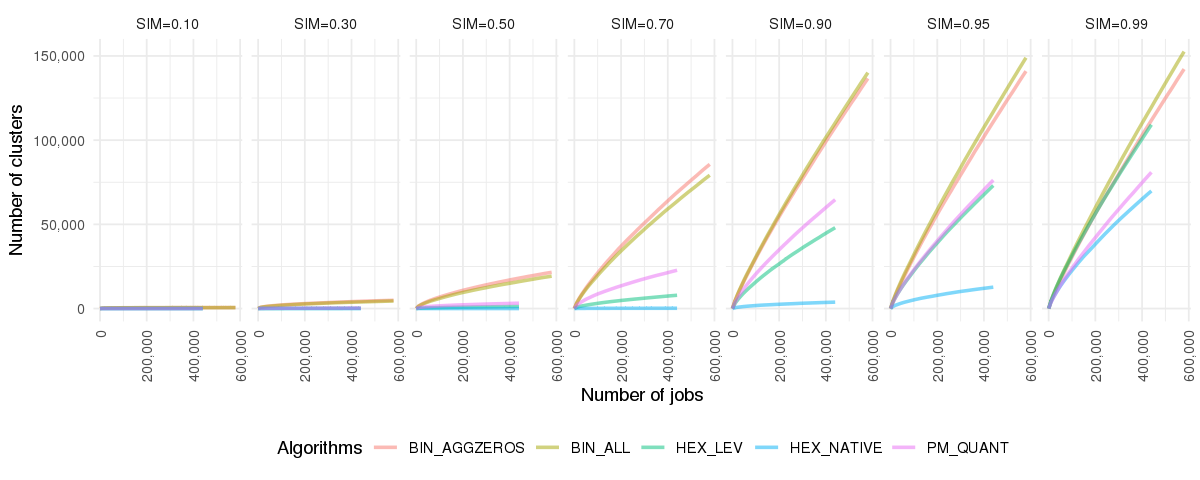
\includegraphics[width=4.61in,height=1.85in]{image15.png}
   \caption{Clustering progress.}
   \label{fig:clustering_progress}
\end{figure}

\begin{figure}
  \centering
  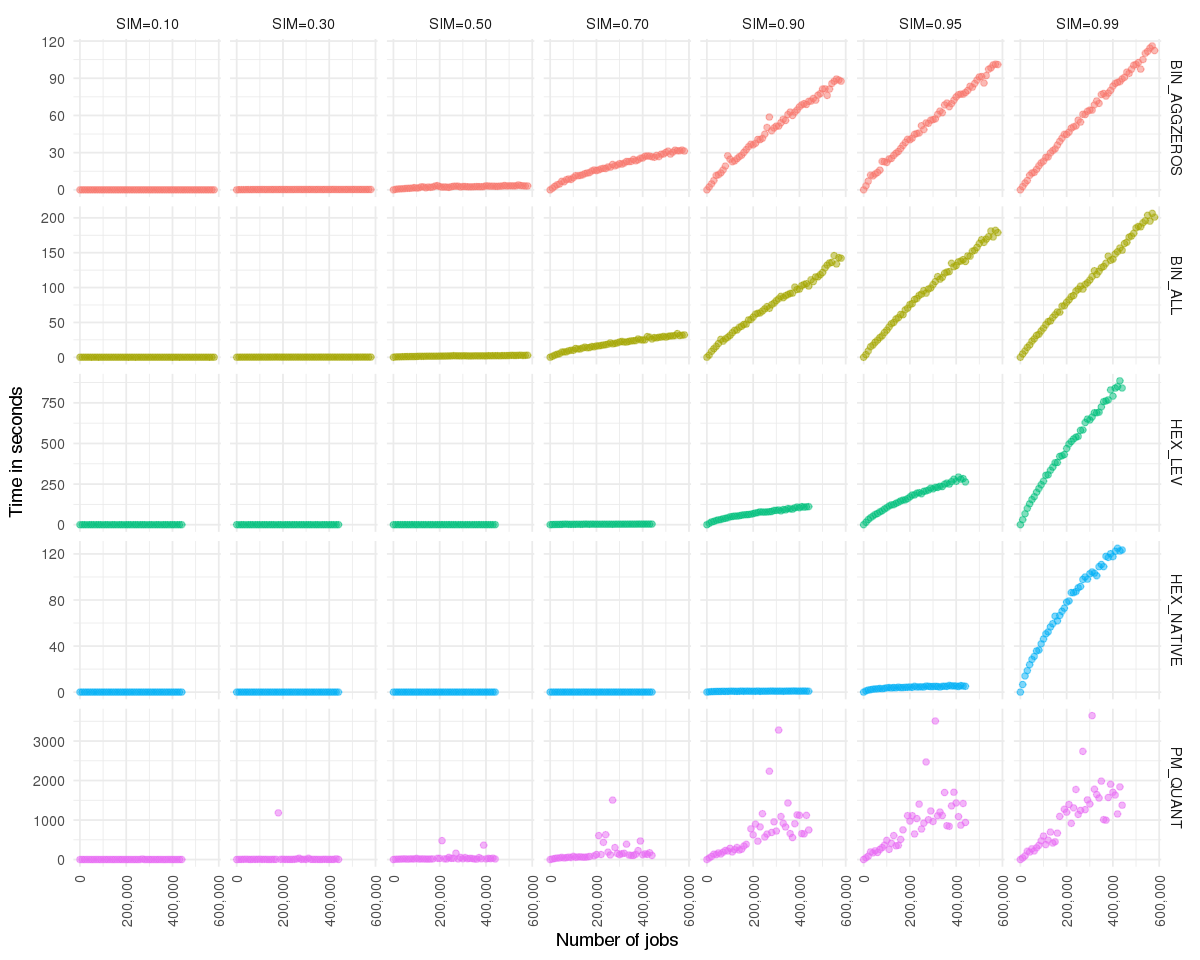
\includegraphics[width=4.61in,height=3.68in]{image18.png}
  \caption{Runtime for executing the clustering.}
  \label{fig:alg_runtimes}
\end{figure}


\begin{figure}
  \centering
  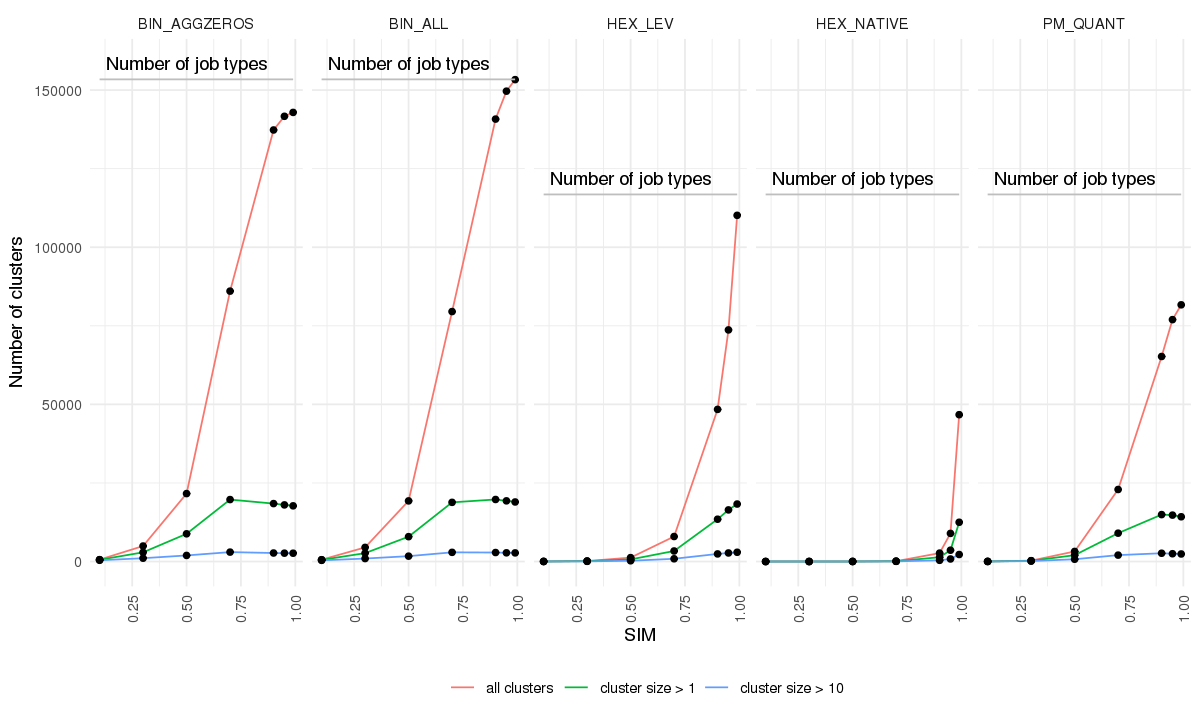
\includegraphics[width=4.61in,height=2.76in]{image19.png}
  \caption{Similarity value exploration.}
  \label{fig:sim_exploration}
\end{figure}

\begin{figure}
  \centering
  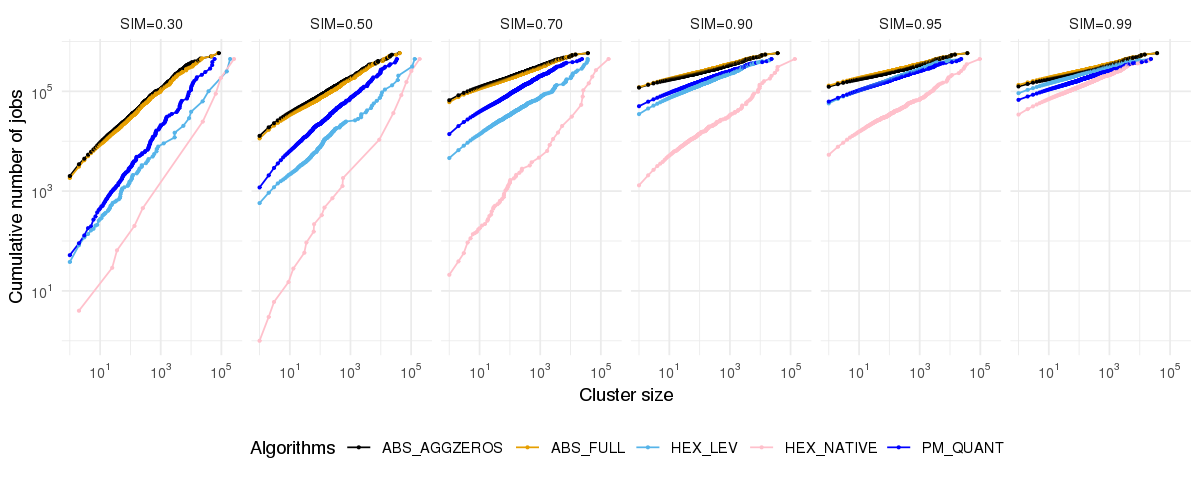
\includegraphics[width=4.61in,height=1.85in]{image22.png}
  \caption{Cumulative number of jobs with different sizes.}
  \label{fig:cum_num_job_sizes}
\end{figure}

\subsection{Cluster Relevance}

To assess the quality of the quantitative clustering better and to aid support staff to identify relevant clusters, we define a relevance of clusters as listed in \Cref{eq:rel}.
The idea behind the relevance definition is the following: the larger the cluster (in terms of jobs) and the longer the jobs, the more potential load these jobs can produce.
Therefore, it is worth investigating these clusters first.
Note that the relevance could include the number of occupied nodes as well to effectively indicate the usage of all jobs on the supercomputer.
In this analysis, we just looked at our definition of weighted relevance.

\begin{equation}
\text{Relevance} = \text{ClusterSize} \cdot \text{MeanJobLength}
\label{eq:rel}
\end{equation}

To give you an impression of cluster qualities for different SIM values, we visualize the Top 10 relevant clusters in \Cref{fig:top10_relevant_jobs}.

The figure confirms that each algorithm creates different clusters as the length of the most relevant clusters and amount is dissimilar.
For a small SIM value, the first few clusters contain a large quantity of shorter (but not so similar) jobs.
However, due to our definition of the relevance metrics, we can observe that smaller clusters with longer jobs are often considered more relevant.
This can be as extreme as a cluster with average length of $>40$ segments is ranked next to one with average length of $1$ segment.
We believe that clustering by relevance (potentially extended by the occupied node number) is useful for support staff to identify optimization potential.

\begin{figure}
  \centering
   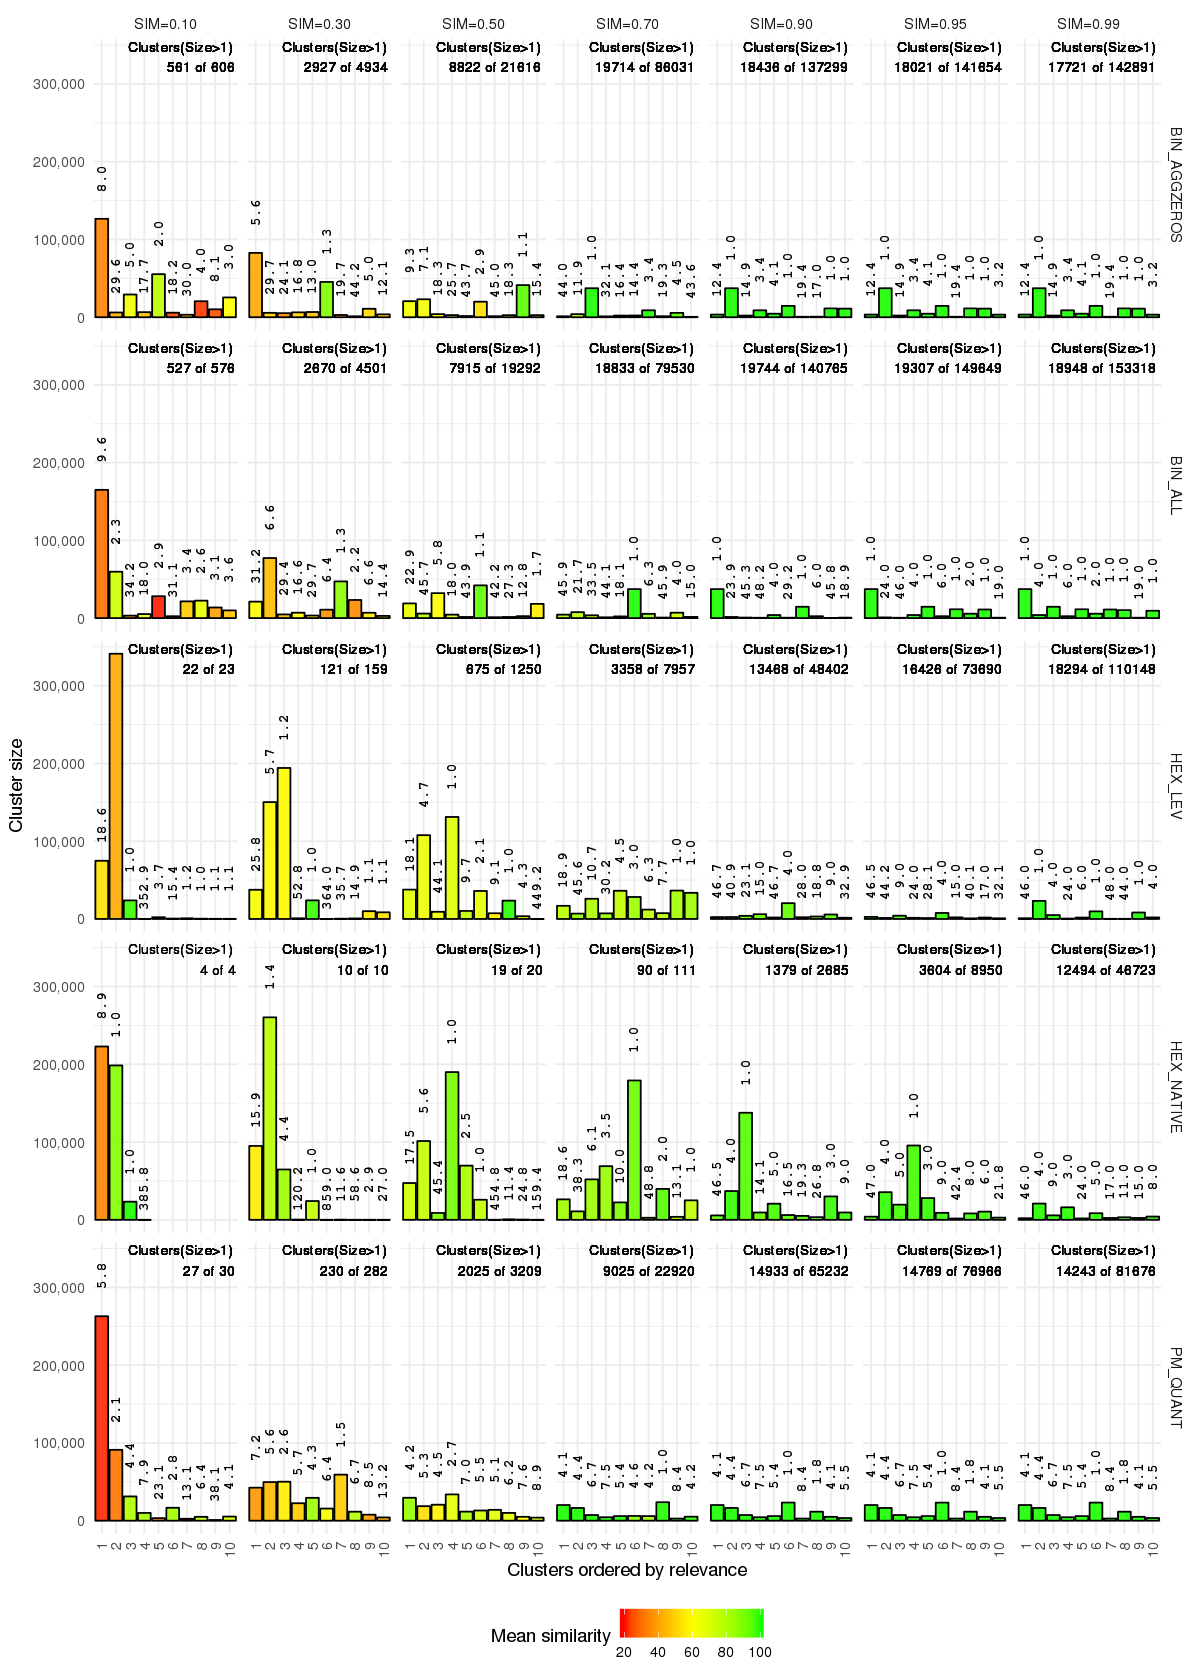
\includegraphics[width=4.61in,height=6.44in]{image11.png}
   \caption{Top 10 relevant jobs ordered by relevance.
   The colors indicate the mean similarity of the jobs in a cluster to the cluster centroid.
   The number above a bar denotes the mean job length of the cluster.}
   \label{fig:top10_relevant_jobs}
\end{figure}

\subsection{Qualitative Evaluation}
The analysis so far does not mean that the quality of the clusters is acceptable.
After manual exploration of selected clusters, we noticed some show a SIM-value independent characteristics.
To explain them, for each algorithm we investigate one cluster of these in detail.

For the presentation of the clusters, we provide a description of particular observations followed by a table containing statistics, then the codings for centroid and most frequent unique jobs in the cluster -- we call such a unique representation a \textit{job phenotype}.
At the end, we include an illustration which describes the segment length distribution of jobs in the cluster that indicates how much the algorithm groups across different job runtime.

\subsubsection{Algorithm characteristics}
The SIM value selection strategy can vary from use case to use case.
As criteria, we choose a SIM value that creates a moderate number of clusters (around 50\% of job phenotypes) and keeps its generalization capabilities (the number of clusters with more than 1 job is considerable).
For the BIN algorithms we chose a SIM of 0.7, and the HEX algorithm SIM of 0.9.

\FloatBarrier
\paragraph{BIN\_ALL}
For the BIN algorithms, we show the statistics of the largest clusters as well in \Cref{tab:bin:largest_clusters} as there is an important aspect.
Looking at \Cref{tab:bin:largest_clusters}, the six largest clusters contain the shortest possible jobs (one segment long).
In each cluster, all jobs have the identical coding; these short running jobs are likely pre/post-processing jobs.

Therefore, the selected cluster for inspection is further down in the Top 5, information is shown in \Cref{cluster:bin_all}.
There are about 3300 different types of unique jobs, it contains jobs with a length between 41 and 60.
Most jobs in the cluster are shorter than 49 segments, because the main Mistral partitions can allocate jobs for at most 8 hours, and that is the majority of jobs.
Since each segment is ten minutes long, the runtime of jobs with 49 segments is about 8.16 hours.
The other jobs must be special allocations.

By inspecting individual jobs in \Cref{cluster:bin_all:top_jobs}, we can see that the centroid has 4 segments $\neq 0$ and the jobs are mostly empty.
As the similarity of 70\% considers empty segments as well, jobs with few I/O segments are found in this cluster.

The following general characteristic observations are made:
\begin{enumerate}
 \item Job phenotypes can significantly differ from centroid and from each other.
 \item Lengths of job phenotypes in a cluster are relatively close to the centroid.
\end{enumerate}

\begin{table}
	\centering
	\begin{tabular}{ll}
		Coding sequence & Cluster size \\
		\midrule
		$[511]$ & 37,272 \\
		$[32]$  & 14,536 \\
		$[272]$ & 11,338 \\
		$[160]$ & 11,014 \\
		$[128]$ & 10,228 \\
		$[8]$   & 9,446  \\
	\end{tabular}
	\caption{BIN algorithm: Top 6 largest clusters created with SIM = 0.7.}
	\label{tab:bin:largest_clusters}
\end{table}

\begin{cluster}
	\begin{subtable}{\textwidth}
		\centering
		\begin{tabular}{lr}
			Number of jobs & 7615 \\
			Number of job phenotypes & 3306 \\
		\end{tabular}
		\caption{Cluster statistics.}
		\label{cluster:bin_all:stats}
	\end{subtable}
	\medskip
	\begin{subtable}{\textwidth}
		\centering
		\begin{tiny}
			\begin{tabular}{l|r}
				\rowcolor{tblhead}
				Binary coding of the centroid                                                                    &  Type     \\
				\hline
				0:0:0:0:0:0:294:0:0:0:0:32:0:0:0:0:0:0:0:0:0:0:0:32:0:0:0:0:0:0:0:0:0:0:0:32:0:0:0:0:0:0:0:0:0:0 &  centroid \\
				\multicolumn{2}{l}{}                                                                             \\
				\rowcolor{tblhead}
				Binary coding of jobs in the cluster                                                             &  Count    \\
				\hline
				0:0:0:0:0:0:359:96:0:0:0:0:0:0:0:0:0:0:0:0:0:0:0:0:0:0:0:0:0:0:0:0:0:0:0:0:0:0:0:0:0:0:0:0:0:0   &  95       \\
				0:0:0:0:0:0:295:0:0:0:0:0:0:0:0:0:0:0:0:0:0:0:0:0:0:0:0:0:0:0:0:0:0:0:0:0:0:0:0:0:0:0:0:0:0:0    &  62       \\
				0:0:0:0:0:0:0:0:0:0:0:0:4:0:0:0:0:0:0:0:0:0:0:0:0:0:0:0:0:0:0:0:0:0:0:0:0:0:0:0:0:0:0:0:0:0:0:0  &  47       \\
				0:0:0:0:0:0:359:0:0:0:0:0:0:0:0:0:0:0:0:0:0:0:0:0:0:0:0:0:0:0:0:0:0:0:0:0:0:0:0:0:0:0:0:0:0:0    &  44       \\
				0:0:0:0:0:6:6:0:0:0:0:0:0:0:0:0:0:0:0:0:0:0:0:0:0:0:0:0:0:0:0:0:0:0:0:0:0:0:0:0:0:0:0:0:0:0:0:0  &  40       \\
			\end{tabular}
		\end{tiny}
		\caption{Centroid and Top 5 job phenotypes.}
		\label{cluster:bin_all:top_jobs}
	\end{subtable}
	\medskip
	\begin{subfigure}{\textwidth}
		\centering
		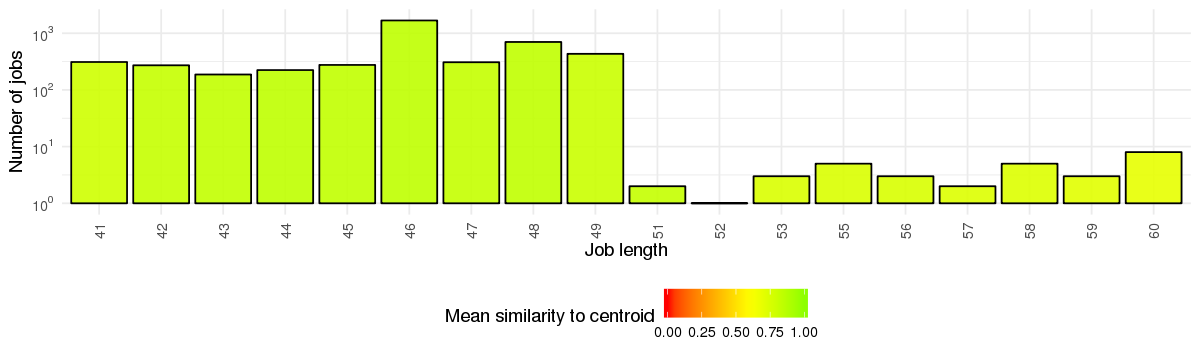
\includegraphics[width=4.61in]{image20.png}
		\caption{Length distribution in the cluster.}
		\label{cluster:bin_all:length}
	\end{subfigure}
	\caption{BIN algorithm: Information of the selected cluster (SIM=0.7).}
	\label{cluster:bin_all}
\end{cluster}

\FloatBarrier
\paragraph{BIN\_AGGZEROS}
The first clusters are identical to BIN, e.g., as shown in \Cref{tab:bin:largest_clusters}.
The reason that both algorithms create the same clusters is that the zero aggregation has no effect on formation of short jobs: the minimum job length required for effective zero aggregation is at least three segments.

We chose again a cluster of the Top 20, information related to the cluster is shown in \Cref{cluster:bin_aggzeros}.
The following is characteristic for this algorithm:

\begin{enumerate}
 \item Job types can significantly differ from centroid and from each other.
 \item Lengths of job phenotypes in a cluster are relatively far from the centroid and compared to BIN\_ALL.
 \item I/O intensive clusters appear to be cleaner than BIN\_ALL.
\end{enumerate}

\begin{cluster}
	\begin{subtable}{\textwidth}
		\centering
		\begin{tabular}{ll}
			\centering
			Number of jobs & 1295 \\
			Number of job phenotypes & 336 \\
		\end{tabular}
		\caption{Cluster statistics.}
		\label{cluster:bin_aggzeros:stats}
	\end{subtable}
	\medskip
	\begin{subtable}{\textwidth}
		\centering
		\begin{tiny}
			\begin{tabular}{l|r}
				\rowcolor{tblhead}
				Binary coding of the centroid                                                                         &  Type     \\
				\hline
				272:272:272:272:272:278:286:272:272:272:272:272:272:272:272:272:272:272:272            &  centroid \\
				\multicolumn{2}{l}{}                                                                   \\
				\hline
				\rowcolor{tblhead}
				Binary coding of jobs in the cluster                                                                          &  Count    \\
				272:272:272:272:272:278:286:272:272:272:272:272:272:272:272:272:272:272:272            &  528      \\
				272:272:272:272:272:406:286:272:272:272:272:272:272:272:272:272                        &  96       \\
				272:272:272:272:272:279:31:272:272:272:272:272:272:272:272:272:272:272:272:272:272:272 &  53       \\
				272:272:272:272:272:272:272:272:272:272:272:279:319:272:272:272:272:272:272:272:272    &  52       \\
				272:272:272:272:272:279:319:272:272:272:272:272:272:272:272:272:272:272:272:272:272    &  50       \\
			\end{tabular}
		\end{tiny}
		\caption{Centroid and Top 5 job phenotypes}
		\label{cluster:bin_aggzeros:top_jobs}
	\end{subtable}
	\medskip
	\begin{subfigure}{\textwidth}
		\centering
		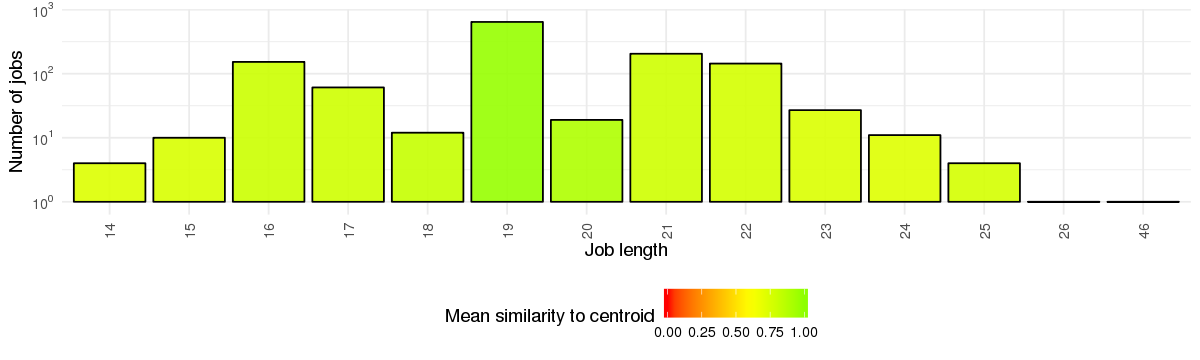
\includegraphics[width=4.61in,height=1.38in]{image13.png}
		\caption{Job length distribution in the cluster.}
		\label{cluster:bin_aggzeros:length}
	\end{subfigure}
	\caption{BIN\_AGGZEROS algorithm: Information of the selected cluster (SIM=0.7).}
	\label{cluster:bin_aggzeros}
\end{cluster}


\FloatBarrier
\paragraph{HEX\_LEV}
Due to the longer hexadecimal codings, smaller changes in the SIM value don't change the clusters as quickly,  compared to binary codings.
Therefore, for this exploration, we chose a SIM value higher than for BIN algorithms.

General cluster characteristics:
\begin{enumerate}
 \item Similar job lengths.
 \item Mostly clean clusters, but a cluster can contain outlier jobs.
\end{enumerate}

We observe that even with a high SIM value some jobs have a different I/O behavior than the centroid and the rest of the jobs.
The reason is for the Levenshtein distance the distance between value 1 and 2 is the same as for 1 and 8; however, we would consider the two jobs closer together.

Information related to the selected cluster is provided in \Cref{cluster:hex_lev}.
In the selected cluster, there is mostly one segment of I/O activity.

\begin{cluster}
	\begin{subtable}{\textwidth}
		\centering
		\begin{tabular}{ll}
			\centering
			Number of jobs & 5769 \\
			Number of job phenotypes & 2473 \\
		\end{tabular}
		\caption{Cluster statistics.}
		\label{cluster:hex_lev:stats}
	\end{subtable}
	\medskip
	\begin{subtable}{\textwidth}
		\centering
		\begin{tiny}
			\begin{tabular}{llll|r}
				\rowcolor{tblhead}
				\multicolumn{4}{l|}{Hexadecimal coding} & \\
				\rowcolor{tblhead}
				md\_file\_create  & md\_file\_delete  & md\_mod           & read\_calls       & Type     \\
				\hline
				0:...:0           & 0:0:0:1:0:0:0:0:0 & 0:...:0           & 0:...:0           & centroid \\
				\multicolumn{5}{l}{}\\
				\rowcolor{tblhead}
				md\_file\_create  & md\_file\_delete  & md\_mod           & read\_calls       & Count    \\
				\hline
				0:...:0           & 0:0:0:0:0:0:1:0:0 & 0:...:0           & 0:...:0           & 606      \\
				0:...:0           & 0:0:0:0:0:0:0:0:1 & 0:...:0           & 0:...:0           & 562      \\
				0:...:0           & 0:...:0           & 0:...:0           & 0:0:0:0:0:0:1:0:0 & 429      \\
				0:...:0           & 0:0:0:1:0:0:0:0:0 & 0:...:0           & 0:...:0           & 185      \\
				0:0:0:0:0:0:1:1:1 & 0:...:0           & 0:0:0:0:0:0:1:0:0 & 0:...:0           & 75       \\
			\end{tabular}
		\end{tiny}
		\caption{Centroid and Top 5 job phenotypes. The metrics that have no I/O activity are not included in the table.}
		\label{cluster:hex_lev:top_jobs}
	\end{subtable}
	\medskip
	\begin{subfigure}{\textwidth}
		\centering
		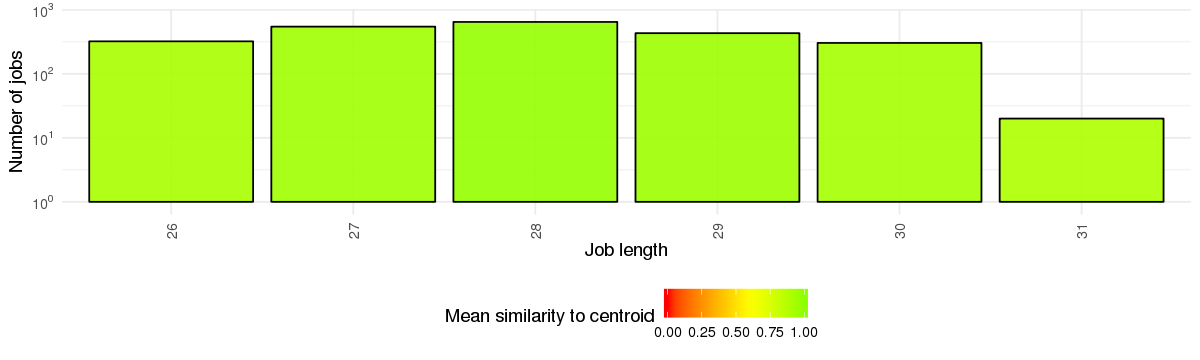
\includegraphics[width=4.61in,height=1.39in]{image5.png}
		\caption{Length distribution in the cluster.}
		\label{cluster:hex_lev:length}
	\end{subfigure}
	\caption{HEX algorithm: Information of the selected cluster (SIM=0.9).}
	\label{cluster:hex_lev}
\end{cluster}


\FloatBarrier
\paragraph{HEX\_NATIVE}
The SIM value exploration shows that this algorithm works best with high SIM values.
Clustering with SIM=0.99 results in clusters that have equal job lengths.
From the definition of the equation, for a similarity of 99\% the centroid must be longer than 100 segments to attract jobs with 99 or 101 length.

General cluster characteristics:
\begin{enumerate}
 \item Similar job lengths (even for lower SIM).
 \item Jobs are relatively close to the centroid.
 \item Low number of outliers.
\end{enumerate}

Information related to the selected cluster is given in \Cref{cluster:hex_native}.
In the selected cluster, jobs with a length of 4 have mostly 1 the activity of one segment in common.

%\jk{Wie kann man das verstehen, obwohl sich der Kasten in zwei Kästen unterscheidet ist das immer noch 99\% ähnlich. Warum haben wir eigtl. nicht die selbe SIM gewählt? 99\% finde ich recht unglücklich für das Beispiel.}

%\begin{myverbbox}[\tiny]{\verbA}
%Gegeben sei zwei hexadecimale Codings fuer zwei Jobs:
%job1 = \left[ 0\dots0], [0\dots0], [0\dots0], [0\dots0], [0\dots0], [0\dots0], [0\dots0], [0:0:1:0], [0:0:1:0]]
%job2 = \left[ 0\dots0], [0\dots0], [0\dots0], [0\dots0], [0\dots0], [0\dots0], [0\dots0], [0:0:0:0], [0:0:2:0]]

%Aenhlichkeit einzelner Metriken:
%metric\_1 = 100%
%metric\_2 = 100%
%metric\_3 = 100%
%metric\_4 = 100%
%metric\_5 = 100%
%metric\_6 = 100%
%metric\_7 = 100%
%md\_mod = (16-(0-0) + 16-(0-0) + 16-(1-0) + 16-(0-0))/(16*4) = 98,4%
%md\_other = (16-(0-0) + 16-(0-0) + 16-(2-1) + 16-(0-0))/(16*4) = 98,4%

%Die Gesamtaehnlichkeit ist dann die folgende:
%similarity = (100*7 + 98,4*2)/9 = 99.65%
%\end{myverbbox}

%\eb{
%  Beispiel: \\
%  \begin{tiny}
%    \verbA
%  \end{tiny}
%}


\begin{cluster}
	\begin{subtable}{\textwidth}
		\centering
		\begin{tabular}{ll}
			Number of jobs & 20908 \\
			Number of job phenotypes & 11997 \\
		\end{tabular}
		\caption{Cluster statistics.}
		\label{cluster:hex_native:stats}
	\end{subtable}
	\medskip
	\begin{subtable}{\textwidth}
		\centering
		\begin{tiny}
			\begin{tabular}{lll|r}
				\rowcolor{tblhead}
				\multicolumn{3}{l|}{Hexadecimal coding} &            \\
				\rowcolor{tblhead}
				md\_file\_delete     &  md\_mod   & md\_other & Type     \\
				\hline
				0:\dots:0            &  0:0:1:0   & 0:0:1:0   & centroid \\
				\multicolumn{4}{l}{} \\
				\rowcolor{tblhead}
				md\_file\_delete     &  md\_mod   & md\_other & Count    \\
				\hline
				0:\dots:0            &  0:\dots:0 & 0:0:1:0   & 5,010    \\
				0:\dots:0            &  0:\dots:0 & 0:0:2:0   & 1,963    \\
				0:0:1:0              &  0:\dots:0 & 0:\dots:0 & 1,099    \\
				0:\dots:0            &  0:\dots:0 & 0:1:0:0   & 911      \\
				0:0:1:0              &  0:0:1:0   & 0:\dots:0 & 676      \\
			\end{tabular}
		\end{tiny}
		\caption{Centroid and Top 5 job phenotypes.}
		\label{cluster:hex_native:top_jobs}
	\end{subtable}
	\medskip
	\begin{subfigure}{\textwidth}
		\centering
		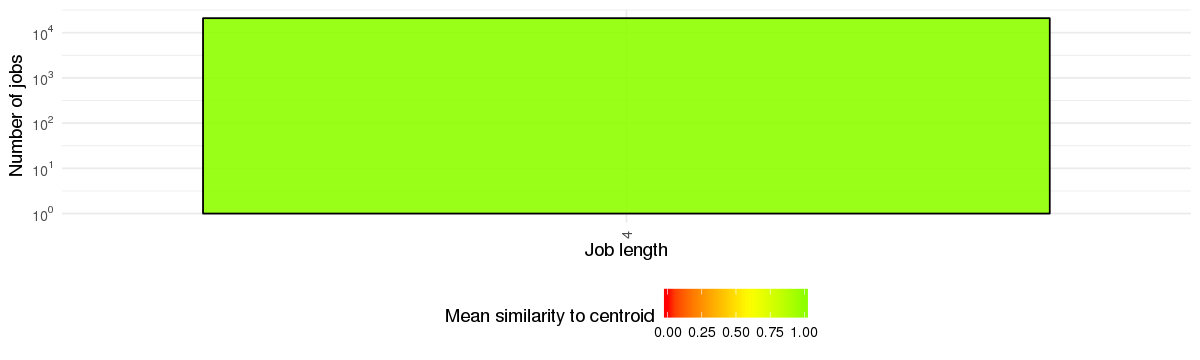
\includegraphics[width=4.61in,height=1.39in]{image8.png}
		\caption{Length distribution in the cluster.}
		\label{cluster:hex_native:length}
	\end{subfigure}
	\caption{HEX\_NATIVE algorithm: Information of the selected cluster (SIM=0.99).}
	\label{cluster:hex_native}
\end{cluster}

\FloatBarrier
\paragraph{PM\_QUANT}
Information related to the selected cluster is shown in \Cref{cluster:pm_quant}.
The first thing to mention are the high generalization capabilities of the algorithm, i.e., that many jobs are mapped to a relatively low number of types.
The next typical property is shown in \Cref{cluster:pm_quant:length}, where we can see that almost the full range of job lengths is represented in the cluster.
This happens, because the PM ignores zero segments.
The aggregation of zero segments is important as most jobs have few I/O phases, in contrast to BIN\_AGGZEROS, it works more efficient.
For example, for PM, the job phenotypes in \Cref{cluster:pm_quant:top_jobs} in the row one and two are 100$\%$ similar.
The centroid and the jobs contain quite similar I/O patterns.

General cluster characteristics:
\begin{enumerate}
 \item Low number of job phenotypes represented in a cluster.
 \item Relatively large number of job lengths represented in a cluster.
 \item I/O pattern of jobs in a cluster are similar.
\end{enumerate}

\begin{cluster}
	\begin{subtable}{\textwidth}
	 \centering
	 \begin{tabular}{ll}
		 Number of jobs & 5175 \\
		 Number of job phenotypes & 154 \\
	 \end{tabular}
	 \caption{Cluster statistics.}
	 \label{cluster:pm_quant:stats}
	\end{subtable}
	\medskip
	\begin{subtable}{\textwidth}
	 \centering
	 \begin{tiny}
		 \begin{tabular}{ll|r}
			 \rowcolor{tblhead}
			 \multicolumn{2}{l|}{Hexadecimal coding} &              \\
			 \rowcolor{tblhead}
			 md\_file\_delete     &  md\_mod     & Type     \\
			 \hline
			 4:0:0:0:0:0          &  4:0:0:0:0:0 & centroid \\
			 \multicolumn{3}{l}{} \\
			 \rowcolor{tblhead}
			 md\_file\_delete     &  md\_mod     & Count    \\
			 \hline
			 4                    &  4           & 2329     \\
			 4:0:0:0:0:0          &  4:0:0:0:0:0 & 1773     \\
			 4:0                  &  4:0         & 224      \\
			 2                    &  4           & 65       \\
			 0:4                  &  0:4         & 57       \\
		 \end{tabular}
	 \end{tiny}
	 \caption{Centroid and Top 5 job phenotypes.}
	 \label{cluster:pm_quant:top_jobs}
	\end{subtable}
	\medskip
	\begin{subfigure}{\textwidth}
		\centering
		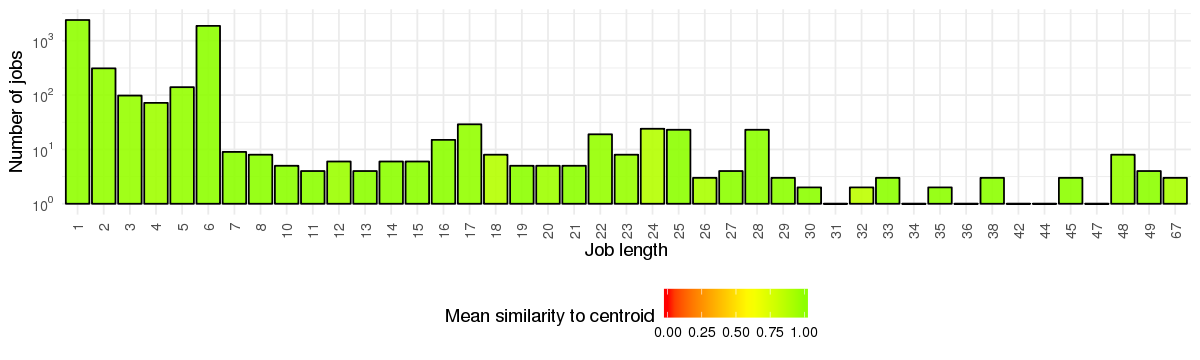
\includegraphics[width=4.61in]{image21.png}
		\caption{Length distribution in the cluster.}
		\label{cluster:pm_quant:length}
	\end{subfigure}
	\caption{PM\_QUANT algorithm: Information of the selected cluster (SIM=0.7).}
	\label{cluster:pm_quant}
\end{cluster}

\FloatBarrier
\subsection{Use Case: Tracking an I/O-Intensive Job}
The demonstration in this section shows how this approach can be used to identify a cluster of I/O-intensive jobs similar to an existing job.

\begin{figure}
  \centering
  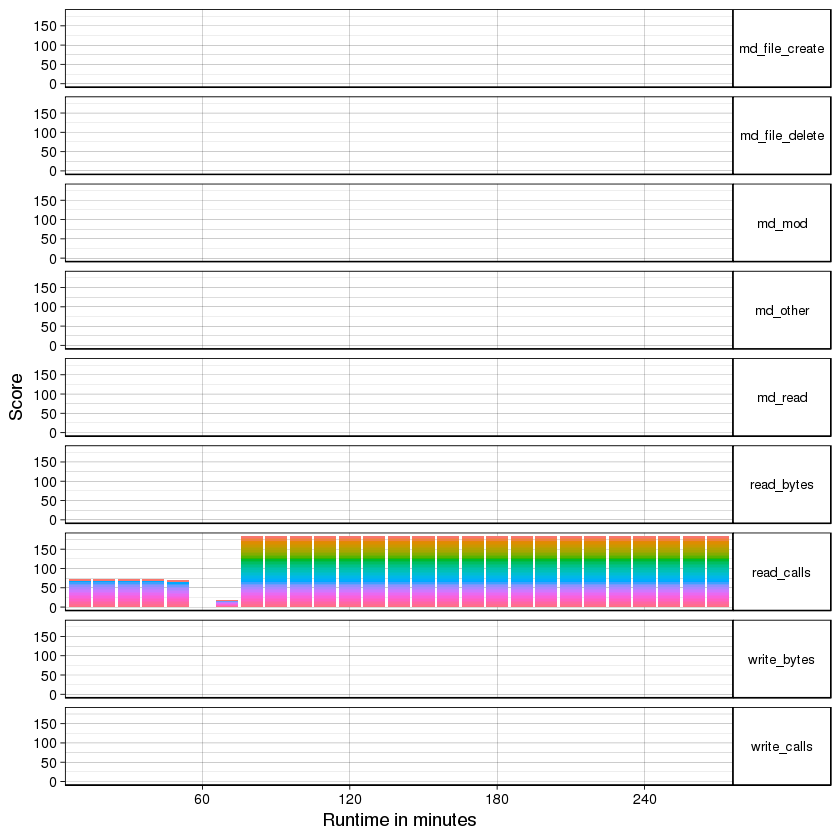
\includegraphics[width=2.84in,height=2.85in]{image1.png}
  \caption{One high I/O intensity job running on 46 nodes.
Score is the sum of all nodes stacked by the node.
A color represents one of the nodes.}
  \label{fig:use_case}
\end{figure}

Firstly, we find an I/O intensive job that we use to identify similar jobs.
The selected job is visualized in \Cref{fig:use_case}.
This relatively long job (27~segments) reveals one heavily used metric.
The job reads data over its runtime but doesn't have any noteworthy activities in any other metrics.
At beginning, only a subset of the nodes is reading most of the data, later more nodes participate in the reading.
The amount of transmitted data is not large but the number of read calls is high and may potentially degrade the file system performance.
Now, we identify and investigate the cluster that contains this job for the different algorithms and discuss if these jobs are similar.

Overall, we find this job leads to good conditions for all algorithms, i.e., all the algorithms work well in this use case.

\FloatBarrier
\paragraph{BIN\_ALL}
Information related to the cluster of the job is in \Cref{cluster:use_case:bin}.
We find that the identified jobs in the cluster are sufficiently related.

\begin{cluster}
	\begin{subtable}{\textwidth}
		\centering
		\begin{tabular}{ll}
			Number of jobs & 27 \\
			Number of job phenotypes & 17 \\
		\end{tabular}
		\caption{Cluster statistics.}
		\label{cluster:use_case:bin_all:stats}
	\end{subtable}
	\medskip
	\begin{subtable}{\textwidth}
		\centering
		\begin{tiny}
			\begin{tabular}{l|r}
				\rowcolor{tblhead}
				Binary coding                                                                                          &  Type     \\
				\hline
				192:192:192:192:192:192:196:192:192:192:192:192:192:192:192:192:192:192:192:192:192:192:64:64:64:64:64 &  job      \\
				192:192:192:192:192:192:192:192:192:192:192:454:230:192:192:192:192:192:192:192:192:192:192:192        &  centroid \\
				\multicolumn{2}{l}{}                                                                                   \\
				\rowcolor{tblhead}
				Binary coding                                                                                          &  Count    \\
				\hline
				192:192:192:192:192:454:198:192:192:192:192:192:192:192:192:192:192:192:192:192:192:192:192:192        &  5        \\
				192:192:192:192:192:192:192:192:192:192:192:454:230:192:192:192:192:192:192:192:192:192:192:192        &  3        \\
				192:192:192:192:192:454:230:192:192:192:192:192:192:192:192:192:192:192:192:192:192:192:192:192        &  3        \\
				192:192:192:192:192:192:192:192:192:192:192:454:230:192:192:192:192:192:192:192:192:192:192            &  2        \\
				228:192:192:192:192:192:192:192:192:192:192:192:192:192:192:192:192:192                                &  2        \\
			\end{tabular}
		\end{tiny}
		\caption{Job, centroid and Top 5 job phenotypes.}
		\label{cluster:use_case:bin_all:top_jobs}
	\end{subtable}
	\medskip
	\begin{subfigure}{\textwidth}
		\centering
		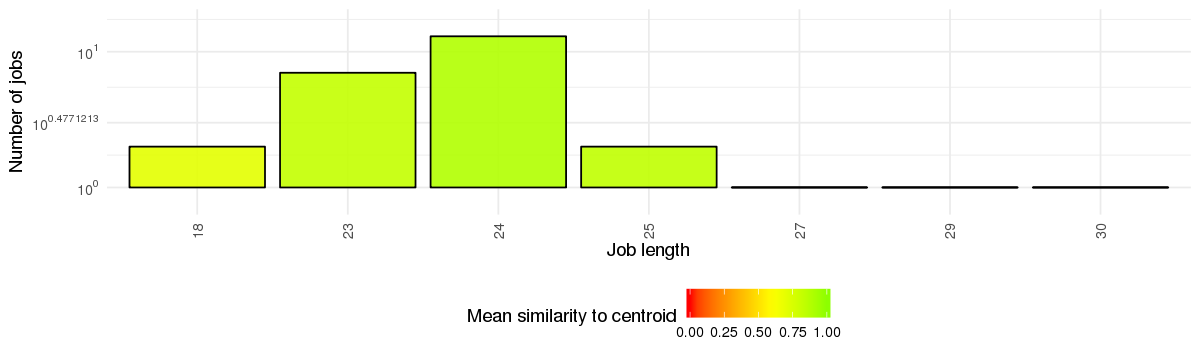
\includegraphics[width=4.61in,height=1.39in]{image9.png}
		\caption{Length distribution in the cluster.}
		\label{cluster:use_case:bin_all:length}
	\end{subfigure}
	\caption{BIN algorithm: Information of the selected cluster (SIM=0.7).}
	\label{cluster:use_case:bin}
\end{cluster}

\FloatBarrier
\paragraph{BIN\_AGGZEROS}
Information related to the cluster is in \Cref{cluster:use_case:bin_aggzeros}.
Compared to BIN, the cluster is smaller but the jobs have a more similar ending.

%\jk{Vl. hätte man einfach nur den Job als Centroid nehmen sollen und Ähnlichkeit aller Jobs dazu feststellen?}
%\eb{Ist eine gute Idee fuer den zweiten Workflow.
%  Die LookUp Operation wuerde allerdings einige Minuten dauern.
%  Nach meiner Vorstellung wird ein Job nach dem Ende sofort einem Cluster zugeordnet.
%  So liegen die Cluster schon bereit.
%  Eine Look-up Operation wuerde dann nur wenige Millisekundne dauern.
%}

\begin{cluster}
	\begin{subtable}{\textwidth}
		\centering
		\begin{tabular}{ll}
			Number of jobs & 8 \\
			Number of job phenotypes & 8 \\
		\end{tabular}
		\caption{table}{Cluster statistics.}
		\label{cluster:use_case:bin_aggzeros:stats}
	\end{subtable}
	\medskip
	\begin{subtable}{\textwidth}
		\centering
		\begin{tiny}
			\begin{tabular}{l|r}
				\rowcolor{tblhead}
				Binary coding                                                                                             &  Type     \\
				\hline
				192:192:192:192:192:192:196:192:192:192:192:192:192:192:192:192:192:192:192:192:192:192:64:64:64:64:64    &  job      \\
				511:238:192:510:192:224:228:192:192:192:192:192:192:192:192:192:192:192:192:192:192:64:64:64:64:64        &  centroid \\
				\multicolumn{2}{l}{}                                                                                      \\
				\rowcolor{tblhead}
				Binary coding                                                                                             &  Count    \\
				\hline
				0:224:192:192:192:192:228:192:192:192:192:192:192:192:192:192:192:192:192:192:192:64:64:64:64:64          &  1        \\
				192:192:192:192:192:192:196:192:192:192:192:192:192:192:192:192:192:192:192:192:192:192:64:64:64:64:64    &  1        \\
				192:192:193:196:192:192:192:192:192:192:192:192:192:192:192:192:192:192:192:192:64:64:64:64               &  1        \\
				192:193:193:198:192:192:192:192:192:192:192:192:192:192:192:192:192:192:192:192:192:64:64:64:64:64:64     &  1        \\
				207:463:225:495:246:224:198:192:192:192:192:192:192:192:192:192:192:192:192:192:192:192:64:64:64:64:64:64 &  1        \\
			\end{tabular}
		\end{tiny}
		\caption{Job, centroid and Top 5 job phenotypes.}
		\label{cluster:use_case:bin_aggzeros:top_jobs}
	\end{subtable}
	\medskip
	\begin{subfigure}{\textwidth}
		\centering
		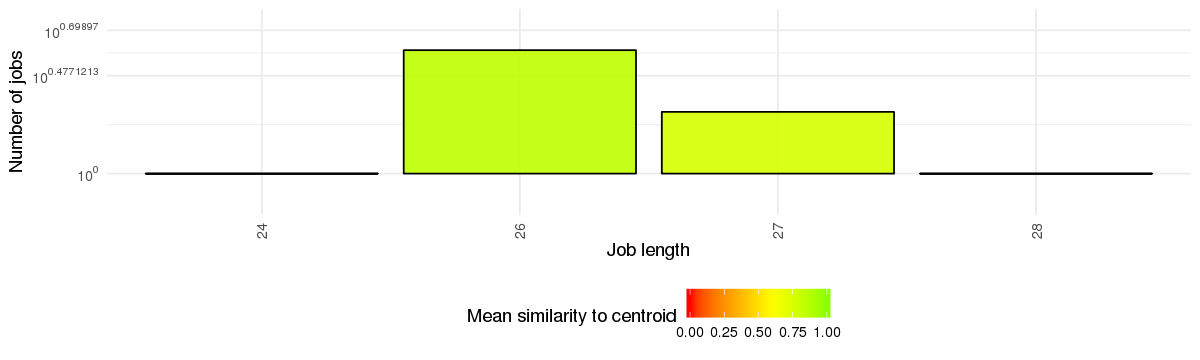
\includegraphics[width=4.61in,height=1.39in]{image6.png}
		\caption{Length distribution in the cluster.}
		\label{cluster:use_case:bin_aggzeros:length}
	\end{subfigure}
	\caption{BIN\_AGGZEROS algorithm: Information of the selected cluster (SIM=0.7).}
	\label{cluster:use_case:bin_aggzeros}
\end{cluster}

\FloatBarrier
\paragraph{HEX\_LEV}
Information related to the cluster is in \Cref{cluster:use_case:hex_lev}.
Overall, the job is matched partially, jobs in the cluster may contain at the beginning an idle phase.

Notice that there is a discrepancy between the job visualization in \Cref{fig:use_case} and the hexadecimal job codings.
While in \Cref{cluster:use_case:hex_lev} we can see a less intensive phase in the beginning and a high intensive phase afterwards, the hexadecimal coding contains a more or less single high intensive I/O phase.
The reason is that we use different reduction functions.
While in the illustration we aggregate segments by the sum() function, for the coding we use mean() function for the same set of values.
While sum() is better for visualization, the mean value allows us to build simple algorithms.

\begin{cluster}
	\begin{subtable}{\textwidth}
		\centering
		\begin{tabular}{ll}
			Number of jobs & 209 \\
			Number of job phenotypes & 189 \\
		\end{tabular}
		\caption{Cluster statistics.}
		\label{cluster:use_case:hex_lev:stats}
	\end{subtable}
	\medskip
	\begin{subtable}{\textwidth}
		\centering
		\begin{tiny}
			\begin{tabular}{ll|r}
				\rowcolor{tblhead}
				\multicolumn{2}{l|}{Hexadecimal coding} & \\
				\rowcolor{tblhead}
				md\_other                                           &  read\_calls                                           & Type     \\
				\hline
				0:\dots:0                                           &  3:3:8:8:8:5:6:8:8:8:8:8:8:8:8:8:8:8:8:8:8:8:8:8:8:8:8 & job      \\
				0:\dots:0                                           &  8:8:8:8:8:2:6:8:8:8:8:8:8:8:8:8:8:8:8:8:8:8:8:8:8:8:8 & centroid \\
				\multicolumn{3}{l}{}                                \\
				\rowcolor{tblhead}      md\_other                   &  read\_calls                                           & Count    \\
				\hline
				0:\dots:0                                           &  0:0:0:0:0:0:8:8:8:8:8:8:8:8:8:8:8:8:8:8:8:8:8:8:8:8   & 4        \\
				0:\dots:0                                           &  8:8:8:8:8:2:8:8:8:8:8:8:8:8:8:8:8:8:8:8:8:8:8:8:8:8   & 4        \\
				0:0:0:4:0:0:0:0:0:0:0:0:0:0:0:0:0:0:0:0:0:0:0:0:0:0 &  0:0:0:0:0:0:8:8:8:8:8:8:8:8:8:8:8:8:8:8:8:8:8:8:8:8   & 4        \\
				0:\dots:0                                           &  8:8:8:8:8:3:8:8:8:8:8:8:8:8:8:8:8:8:8:8:8:8:8:8:8:8:8 & 3        \\
				0:\dots:0                                           &  0:0:0:0:0:0:2:8:8:8:8:8:8:8:8:8:8:8:8:8:8:8:8:8:8:8   & 2        \\
			\end{tabular}
		\end{tiny}
		\caption{Job, centroid and Top 5 job phenotypes.}
		\label{cluster:use_case:hex_lev:top_jobs}
	\end{subtable}
	\medskip
	\begin{subfigure}{\textwidth}
		\centering
		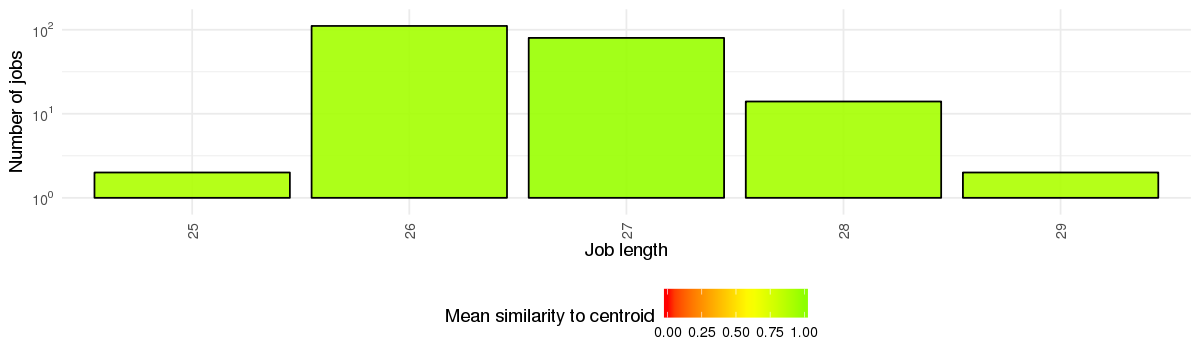
\includegraphics[width=4.61in]{image17.png}
		\caption{Length distribution in the cluster.}
		\label{cluster:use_case:hex_lev:length}
	\end{subfigure}
	\caption{HEX\_LEV algorithm: Information of the selected cluster (SIM=0.9).}
	\label{cluster:use_case:hex_lev}
\end{cluster}

\FloatBarrier
\paragraph{HEX\_NATIVE}
Information related to the cluster is in \Cref{cluster:use_case:hex_native}.
Again, the jobs look similar, however, the increase in performance and drop in segment\,5 is not captured.

\begin{cluster}
	\begin{subtable}{\textwidth}
		\centering
		\begin{tabular}{ll}
			Number of jobs & 20 \\
			Number of job phenotypes & 20 \\
		\end{tabular}
		\caption{Cluster statistics.}
		\label{cluster:use_case:hex_native:stats}
	\end{subtable}
	\medskip
	\begin{subtable}{\textwidth}
		\centering
		\begin{tiny}
			\begin{tabular}{l|r}
				\rowcolor{tblhead}
				Hexadecimal coding & \\
				\rowcolor{tblhead}
				read\_calls                                           & Type     \\
				\hline
				3:3:8:8:8:5:6:8:8:8:8:8:8:8:8:8:8:8:8:8:8:8:8:8:8:8:8 & job      \\
				8:8:8:8:8:2:4:8:8:8:8:8:8:8:8:8:8:8:8:8:8:8:8:8:8:8:8 & centroid \\
				\multicolumn{2}{l}{}\\
				\rowcolor{tblhead}
				read\_calls                                           & Count    \\
				\hline
				8:8:8:8:8:3:8:8:8:8:8:8:8:8:8:8:8:8:8:8:8:8:8:8:8:8:8 & 3        \\
				8:8:8:8:8:5:8:8:8:8:8:8:8:8:8:8:8:8:8:8:8:8:8:8:8:8:8 & 2        \\
				3:3:8:8:8:5:6:8:8:8:8:8:8:8:8:8:8:8:8:8:8:8:8:8:8:8:8 & 1        \\
				3:6:6:7:7:7:7:8:8:8:8:8:8:8:8:8:8:8:8:8:8:8:8:8:8:8:8 & 1        \\
				6:5:6:7:6:2:7:8:8:8:8:8:8:8:8:8:8:8:8:8:8:8:8:8:8:8:8 & 1        \\
			\end{tabular}
		\end{tiny}
		\caption{Job and centroid coding sequences.}
		\label{cluster:use_case:hex_native:job_centroid}
	\end{subtable}
	\medskip
	\begin{subfigure}{\textwidth}
		\centering
		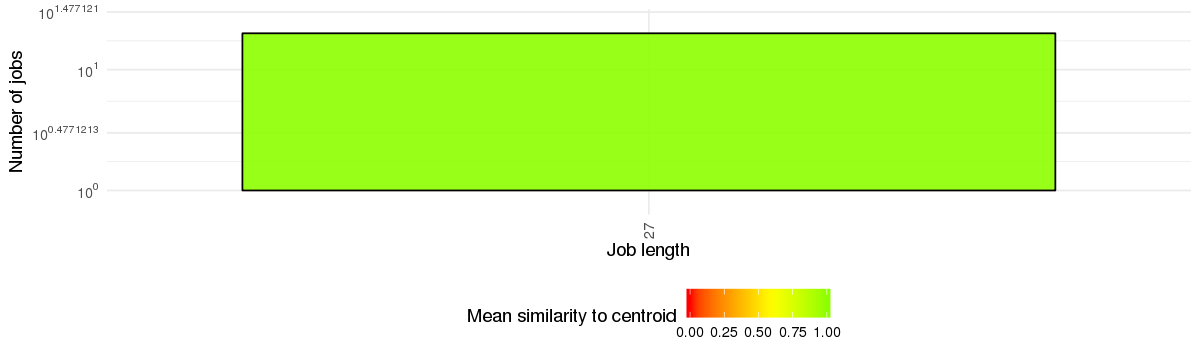
\includegraphics[width=4.61in]{image2.png}
		\caption{Length distribution in the cluster.}
		\label{cluster:use_case:hex_native:length}
	\end{subfigure}
	\caption{HEX\_NATIVE algorithm: Information of the selected cluster (SIM=0.99).}
	\label{cluster:use_case:hex_native}
\end{cluster}

\FloatBarrier
\paragraph{PM\_QUANT}
Information\ related to the cluster is in \Cref{cluster:use_case:pm_quant}.
Even with a smaller SIM value, the jobs appear related while they cover a variety of job length as well.

\begin{cluster}
	\begin{subtable}{\textwidth}
		\centering
		\begin{tabular}{ll}
			Number of jobs      & 68  \\
			Number of job phenotypes & 59  \\
		\end{tabular}
		\caption{Cluster statistics.}
		\label{cluster:use_case:pm_quant:stats}
	\end{subtable}
	\medskip
	\begin{subtable}{\textwidth}
		\centering
		\begin{tiny}
			\begin{tabular}{l|r}
				\rowcolor{tblhead}
				Hexadecimal coding & \\
				\rowcolor{tblhead}
				read\_calls                                           & Type     \\
				\hline
				3:3:8:8:8:5:6:8:8:8:8:8:8:8:8:8:8:8:8:8:8:8:8:8:8:8:8 & job      \\
				8:8:8:8:8:8:8:8:8:8:8:8:8:8:8:8:8:8:8:8:8:8:8:8:8:8   & centroid \\
				\multicolumn{2}{l}{}\\
				\rowcolor{tblhead}
				read\_calls                                           & Count    \\
				\hline
				8:8:8:8:8:2:8:8:8:8:8:8:8:8:8:8:8:8:8:8:8:8:8:8:8:8   & 4        \\
				8:8:8:8:8:3:8:8:8:8:8:8:8:8:8:8:8:8:8:8:8:8:8:8:8:8:8 & 3        \\
				7:7:7:7:7:2:8:8:8:8:8:8:8:8:8:8:8:8:8:8:8:8:8:8:8:8   & 2        \\
				8:8:8:8:8:5:8:8:8:8:8:8:8:8:8:8:8:8:8:8:8:8:8:8:8:8   & 2        \\
				8:8:8:8:8:8:8:8:8:8:8:8:8:8:8:8:8:8:8:8:8:8:8:8:8:8   & 2        \\
			\end{tabular}
		\end{tiny}
		\caption{Job, centroid and Top 5 job phenotypes.}
		\label{cluster:use_case:pm_quant:top_jobs}
	\end{subtable}
	\medskip
	\begin{subfigure}{\textwidth}
		\centering
		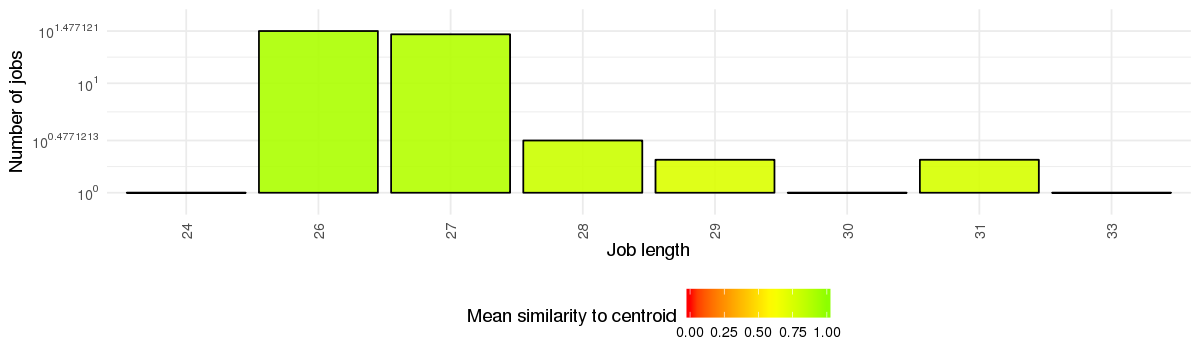
\includegraphics[width=4.61in,height=1.39in]{image7.png}
		\caption{Length distribution in the cluster.}
		\label{cluster:use_case:pm_quant:length}
	\end{subfigure}
	\caption{PM\_QUANT algorithm: Information of the selected cluster (SIM=0.7).}
	\label{cluster:use_case:pm_quant}
\end{cluster}


\FloatBarrier
\subsection{Discussion}
We evaluated similarity between jobs quantitatively and qualitatively for the different algorithms.
As most jobs contain only a subset of I/O-intensive segments, the assessment of similarity should ignore these phases.
There may be specific use cases where the exact job-length play a role but generally it appears that a user or support member should be interested in similar I/O-patterns as otherwise the clusters will be polluted with  irrelevant jobs.

\paragraph{Coding.} The coding of the time series data has a big impact on the potential similarity that can be uncovered.
We explored binary, hexadecimal, and the native (floating-point, e.g., mean) values.

We noticed in the experiments with native coding that the amount of generated clusters skyrocketed.
The reason is that similarity for short jobs exceed a high SIM value quickly and this leads to the creation of new clusters, which in turn leads to long clustering runtimes.
An example illustrates a typical case:
Assume there are two jobs: one running on 16 nodes and other running on 32 nodes.
Both are one segment long and only one I/O node that writes data to storage with a moderate performance.
Without quantization, we would represent these jobs by the following sequences:  [..., [0.0625], $ \ldots $ ] and [..., [0.03125], ...], where only active metrics have values larger than zero.
Using the similarity function without quantization, i.e., with mean performance, would result in a similarity of 50$\%$, and for SIM $>0.5$ they would be placed in separate clusters.

The hexadecimal coding quantizes the data, making them identical, and filters many jobs automatically.
Segments with mean performance less than 0.125 are rounded to zero and zero sequences are removed from the dataset.

Rounding is not necessary for PM.
It can work directly with floating-point numbers.
As it generalized better for smaller similarity, it wouldn't create that many clusters as for the other methods.
The initial motivation behind the use of hexadecimal coding was to apply string methods such as Levenshtein and make data comparable with other algorithms.
%For example, this allows us to see how the additional features affect the quality of clusters.
%By accident, this was also the right decision.


%It also needs to be investigated, if these considerations are correct for HPC systems that are running hundreds of jobs in parallel, because one job alone would typically not be able to produce a significant amount of I/O that can slow down the file system performance.

\medskip

\paragraph{Lengths-invariance.}
With the Levensthein distance, we attempted to resolve this issue allowing to assign jobs of different length into the same cluster.
However, the Levenshtein distance cannot consider the performance of a segment.
For example, the following three codings would be considered to be all different by one symbol, since they differ in one position only.

\begin{lstlisting}
phase_coding_1 : [2:2:2:2:2:9:2:2]
phase_coding_2 : [2:2:2:2:2:8:2:2]
phase_coding_3 : [2:2:2:2:2:0:2:2]
\end{lstlisting}

Intuitively, we would say that {phase\_coding\_1 and{ phase\_coding\_2 are more similar than {phase\_coding\_2 and {phase\_coding\_3, because the difference at 6th position is smaller between Job\,8 and 9 is smaller than to Job\,3.
Short runtimes lead to more polluted clusters.

Here is another example that illustrated the issue of noise in clusters for Levensthein:
Suppose two jobs [0:6:0:0] and [0:388:174:0] are in the same cluster with the centroid [0:388:0:0].
Even if in both cases the similarity between the cluster and the centroid is 75$\%$  (only one change is required), we would intuitively say that these jobs are completely different, not even close to the 75$\%$  mark.
We can easily construct another sequence, e.g., [0:389:0:0], where a similarity of 75$\%$  are justified.
For this reason, we found that the Levenshtein distance is generally not suitable.

\medskip

The current version of the PM algorithm ignores NonIO parts (sequences of zeros) of the monitoring data, and  handles segment sequences like [0,0,0,0,1] and [1] equally:
\begin{lstlisting}
job1_metric1 : [0,0,0,0,1]
job1_metric1 : [1]
\end{lstlisting}

These sequences would produce different average I/O loads on the storage.
Intuitively, we would judge these jobs have different I/O behaviour as the ratio between computational and I/O load is different.

One could argue that the phase definition was chosen incorrectly.
Currently, phases are defined for each metric individually, without consideration of the overall behavior on  other metrics.
For illustration, consider the following two jobs:
\begin{lstlisting}
job1_metric1 : [0:1]
job1_metric2 : [1:0]
job2_metric1 : [1:0]
job2_metric2 : [1:0]
\end{lstlisting}

Currently, the algorithm recognizes the I/O patterns to be 100$\%$ similar.
Alternatively, one could say that running two metrics at the same time is another I/O pattern, as running them shifted, because on a storage system the jobs would produce different I/O loads.
For jobs with many I/O phases, this situation is less likely but for shorter jobs, it may happen.
The benefit of ignoring these aspects is simplicity; this clustering reduces the number of clusters and  results are easier to understand.

\paragraph{Characterization of I/O.}
The main questions for a user that applies a clustering algorithm remain: how to define similarity.
Depending on the use case, the relevant I/O-behavior and characteristics involved in job comparison must be defined to allow identification of jobs depending on temporal behavior.
In our case, we discussed similarity based on profiles and time series data.
We explored various variants for the handling of fluctuation in the time series data that consider time series of different length, omit empty phases, and allow some reordering of phases.
To answer these questions, a discussion with the community about the use cases and a study of more use cases is necessary.


\section{Conclusion}%
\label{sec:conclusion}

In this work, we described various approaches to cluster 1 million jobs based on their I/O behavior.
Clustering of jobs is important for data-center support staff to focus their effort on relevant jobs.
Therefore, we pre-processed the periodically gathered node metrics by converting this fine-grained resolution into 10-minute segments using various pre-processing stacks.
Our contribution is the systematic evaluation and discussion of various approaches for the clustering.
The success of clustering algorithms depends on the right feature selection and data transformation.

After a series of experiments with general purpose algorithms, we could not achieve suitable results.
While we could have applied traditional approaches such as k-means on the data, we found that the large number of classes and unknown knowledge about the jobs doesn't suit this use case.
One problem might be that we apply a combination of a clustering and a classification algorithm.
The classification algorithm is trained by the potential erroneous output of the clustering algorithm and it can itself produce erroneous output, which multiples the total error.
Even if a better solution would found there is no guarantee that the generated model could be applied on another system.

In the evaluation, we investigated the quantitative and qualitative behavior of different algorithms.
The investigation of clusters shows that, particularly clusters with little I/O activity are noisy and do not meet our expectation.
Depending on the similarity chosen by the user, there are many different clusters with phenotypes of jobs found.
Thus, exceeding the ability for manual inspection and manual labeling.

Our analysis shows that considering the relative I/O performance and I/O phases improves the clustering.
The integration of the awareness of I/O performance produces better, but still not sophisticated results.
Therefore, we found that the Levenshtein distance is generally not suitable for similarity of I/O behavior of jobs.

Absolute coding aggregates three dimensions (Metric, Nodes, and FileSystems) resulting in a nine times shorter coding sequence than hexadecimal coding, which aggregates only two dimensions (Nodes, and FileSystems).
Using hexadecimal coding is more precise than binary coding because hexadecimal coding sequences longer.
However, using the actual native floating-point value is problematic for the developed algorithms as for high similarity it will generate too many clusters.
Therefore, we consider the quantization of hexadecimal is appropriate for this use case.

The phase matching algorithm detects phases and differentiates performance values.
In our analysis, it produced even for smaller relative similarity good results.
These algorithms can be used in practice to identify jobs similar to another.
We defined the cluster relevance that aids data center employees to select jobs of relevance.
%Due to the huge amount of clusters and lack of automatic evaluation tools, we can not prove this statement for all clustres.
%This makes training of models a trial-and-error approach.


\subsection{Future Work}
To address the issue with the large number of clusters we will research three additional functions: 1) filter irrelevant clusters, 2) sort clusters by criteria, and 3) automatic labeling.

We intend to conduct a survey and discussion with users to answer the question what similarity of I/O jobs means.
We will extend relevance to cover node count as well to represent the actual costs of running a job better.

We see a high potential in the new clustering algorithms to apply them on the fly to jobs of interest.
For this case, the jobs could be grouped based on distance to this particular job and allowing the user to modify the similarity online.
Conducting a study about this approach is our next goal.


\subsection*{Acknowledgment} %% Remove this section if not needed
\textit{We thank the reviewers XX and YY for the feedback.}

  % The bibliography
\addcontentsline{toc}{section}{Bibliography}
\bibliography{bibliography.bib}

\reviews   % The review section

\subsection*{Reviewer: \href{Optional URL to reviewer page}{Firstname LastName}, Date: 2020-07-07}

\paragraph{Overall summary and proposal for acceptance}

\paragraph{Scope}   % in regards to the journal, i.e., does the topic fit?

\paragraph{Significance}   % of the research, minor vs. major

\paragraph{Readability}   % English and structure appropriate?

\paragraph{Presentation}

\paragraph{References}   % Correctly formatted?

\paragraph{Correctness}   % Is the research correct

\end{document}
